\documentclass[12pt,a4paper,openright]{report}

%\\usepackage\{url,graphicx\}\
\usepackage[pdftex]{graphicx}
\usepackage[bookmarks,%
            a4paper,%
            breaklinks,%
            backref=true,%
            urlcolor=blue,
            linkcolor=blue,
            citecolor=magenta,
            pdfhighlight=/I,%
            pdffitwindow=true,%
            pdfstartview=Fit,%
            pdfcenterwindow=true,%
            pdfborder={0 0 0.5 [2 2]},
            linkbordercolor={0 0 0},%
            %colorlinks,%
            colorlinks=true,
            hyperfootnotes=false,
            %linkcolor={0 0 0},
            urlbordercolor={0 0 0},
            %pdfbordercolor=magenta,
            pdftitle=EQ2440 Project Report,%
            pdfauthor=RedTeam2014]%
            {hyperref}

\renewcommand\thefootnote{\textcolor{red}{\arabic{footnote}}}
\usepackage[english]{babel}
\usepackage[utf8]{inputenc}
\usepackage{amsmath}
\usepackage[margin=2cm]{geometry}
%\usepackage{fullpage}
\usepackage{setspace}
\usepackage{cleveref}
\usepackage{bm}
\onehalfspacing
\usepackage[font=small,labelfont=bf]{caption}
\usepackage{float}
\usepackage{booktabs}
\graphicspath{{expt/}{Graphics/}}
%\usepackage[options]{natbib}
\usepackage{xfrac}
\usepackage{hyperref}
\usepackage{color}
\usepackage[usenames,dvipsnames,svgnames,table]{xcolor}
\usepackage{epstopdf}
\usepackage{graphicx}
\usepackage{times}
\renewcommand{\ttdefault}{lmtt} %tt
\usepackage[boxed]{algorithm2e}
\usepackage{indentfirst}
\usepackage[varg]{txfonts}
\usepackage{caption}
\usepackage{subcaption}
\renewcommand{\descriptionlabel}[1]{\hspace{\labelsep}\boldmath{#1}}
%\renewcommand{\descriptionlabel}[1]{\hspace{\labelsep}\emph{#1}}

%
%\usepackage{listings}
%\usepackage{color} %red, green, blue, yellow, cyan, magenta, black, white
%\definecolor{mygreen}{RGB}{28,172,0} % color values Red, Green, Blue
%\definecolor{mylilas}{RGB}{170,55,241}
\usepackage[utf8]{inputenc} 

%Degree sign
\usepackage{gensymb}
%

\newcommand*{\footnotemarkcolor}{black}

\usepackage{enumitem}

%\usepackage{subfig}
%\usepackage{footnotebackref}
\usepackage{footmisc}
%%% Macro definitions for Commonly used symbols
\newcommand{\etas}{\ensuremath{\eta_{\mathrm{s}}}}
\newcommand{\HRule}{\rule{\linewidth}{0.5mm}}



%ABSTRACT

\usepackage{abstract}
\renewcommand{\abstractnamefont}{\normalfont\Large\bfseries}
\renewcommand{\abstracttextfont}{\normalfont\small}

\renewenvironment{abstract}
  {\small\quotation
  {\bfseries\noindent{\large\abstractname}\par\nobreak\smallskip}}
  {\endquotation}


\begin{document}

\begin{titlepage}
\begin{center}
\textsc{\LARGE Royal Institute of Technology}\\[0.3cm]

\includegraphics[width=0.4\textwidth]{./logo}~\\[0.3cm]


\textsc{\Large Project in Wireless Communications \\ EQ2440}\\[0.5cm]

\HRule \\[0.4cm]
{ \huge \bfseries Project Report \\[0.4cm] }

\HRule \\[1.5cm]

\begin{minipage}{0.4\textwidth}
\begin{flushleft} \large
\emph{Authors:}\\
Alan \textsc{Anter} \\
Daniel \textsc{Bredstedt}\\
Sergio A. \textsc{Chávez Cárdenas}\\
Henrik \textsc{Forsell}\\
Johan \textsc{Ottersten}\\
Francisco \textsc{Rosário}\\
Jue \textsc{Zhang}\\

\end{flushleft}
\end{minipage}
\vfill
{\large \today}



\end{center}
\end{titlepage}


%Empty page after title page
\newpage\null\thispagestyle{empty}\newpage


\begin{abstract}

The usage of mobile phones connected to a base station is strictly forbidden inside airplanes because of the inherent risk of interference with the aircraft navigation or communication systems. For this reason, there is a flight mode in most devices, which turns off all RF signals. However, passengers often have the necessity to transmit files with their phones during the flight and alternatives should be available.

This report describes the way we design and build a communication system capable of transferring files between two smartphones using the devices' sound card and a 3.5 mm audio cable as channel. The system is implemented in real time in an Android application, which allows the user to select a file and send it through the channel to a receiving terminal. All the processing is done by an Android application that runs into Samsung Galaxy S3 devices with Android OS 4.2.1. Additionally, an off-line processing system has been developed and tested with MATLAB to conduct the experiments with the algorithms involved in the file transfer process.

Several digital modulation schemes have been tested together with other different techniques in order to achieve the highest possible throughput at the channel. In real-time, we use a 64-QAM system with a data rate of 33kbps. The processing is done at a reasonable computational time and the algorithms are optimised in order to perform efficiently and detect errors on the transmission. On the other hand, the off-line system has been pushed to the limits to obtain the best possible throughput in the bandwidth limited channel. An OFDM system capable to transmit up to 90kbps is used in this mode instead.  
  


\end{abstract}

\clearpage

%Changes the colour of the links to black
{\hypersetup{hidelinks}\tableofcontents}
{\hypersetup{hidelinks}\listoffigures}
{\hypersetup{hidelinks}\listoftables}
%


%\tableofcontents               with links
%\listoffigures                     with links
%\listoftables                      with links

\clearpage

%Empty page after list of..
\newpage\null\thispagestyle{empty}\newpage

\renewcommand{\abstractname}{Acknowledgements}
\begin{abstract}
 Thanks to the reader, if you are reading this line after the others, you at least read one page of this long report. Thank you.
\end{abstract}

\clearpage




% % % % % % % % % % % % % % % % % % % % % % % % % % % %
% % % % % % % % % % % % % % % % % % % % % % % % % % % %

%Beging of report 
\SetAlgoSkip{bigskip}
\chapter{Introduction}

In a scenario in which mobile wireless communications are restricted, like in the case of being in an airplane, sharing files between mobile devices may not be possible. In previous years, some alternative solutions that do not use RF signals have been explored, such as the usage of the phone speakers and microphone, as well as the camera and the screen (QR codes). The problem with such methods, is that the rate is heavily limited due to channel impairments like external sounds or visual limitations.
In this year’s project, we will use a different approach, which is: to transmit a file using an audio cable. To achieve this, we will use the audio/mic jacks as transceivers and then, connect two phones with a 3.5mm cable to send a modulated audio signal with the file information. The transmission and reception of such file will be managed by the Android application that is to be developed. In this way, we expect to achieve a higher throughput compared with the case of transmitting sound over the air which was only 1.2 kbps \cite{report2012}.

The goal of this project is to implement a system that transmits a file stored in the phone’s SD card to another phone connected with a cable via their audio/mic jacks. Since the audio jacks are limited to the audible frequency range, our overall transmission rate will also be constrained to such range. In addition, we need to test the frequency range of the microphone input to see if it further limits the available bandwidth. Regarding the cable, it should behave as a nearly “ideal” channel (negligible noise and phase delay) inside the working frequencies.
After characterizing our transmitter and receiver, we can design a system that modulates the desired file into a signal, send it through the cable, and do the reverse process (e.g. demodulate, decode) in the other terminal. We will be able to test and characterise our modem at the first stages with MATLAB. 
After we accomplish the modem design, we will use the provided Android framework to implement the file transfer application (client and server). The framework platform is implemented in JAVA, and the Eclipse IDE will be used to build our system. 



% % The following report is organised in the following order:
% % \begin{itemize}
% % \item \bf Chapter \ref{chap:Background}: \textnormal{Background. A general description of the theoretical foundations of the digital systems and techniques that were explored and implemented in our system.}
% % \item \bf Chapter \ref{chap:App}: \textnormal{Android Prototype. A description about of the software and hardware tools that were used to implement our system as well as the details of the methods and functions that were added to the Android framework in order to have a file transfer application.}
% % \item \bf Chapter \ref{chap:method}: \textnormal{Method. A detailed description of the algorithms and tests of the techniques that were studied in chapter \ref{chap:Background}.}
% % \item \bf Chapter \ref{chap:results}: \textnormal{Results and discussion. A compilation of the outcomes of the performed tests as well as a discussion of such results.}
% % \item \bf Chapter \ref{chap:conclusions}: \textnormal{Conclusions. Summary of the general results of the project.}

% \end{itemize}


\chapter{Background} %or Theory
\label{chap:Background}
Before describing the implementation, it is important to study the possible coding and modulation schemes in order to determine the best combination for the given problem. In this section, the fundamental principles of each technique are analysed.

\section{Modulation Schemes}

\subsection{ASK}
Amplitude shift keying (ASK) uses the variations in amplitude of a carrier wave to represent the digital data. The mapping or allocation of $k$ information bits to the $M=2^k$ possible signal amplitudes can be done in different ways. The preferred mapping is the one in which the adjacent  signal amplitudes differ by one binary digit (Gray coding). The simplest case for the transmitted signal, when only two amplitudes coexist, is shown in figure \ref{fig:ask}. 

\begin{figure}[H]
  \centering
    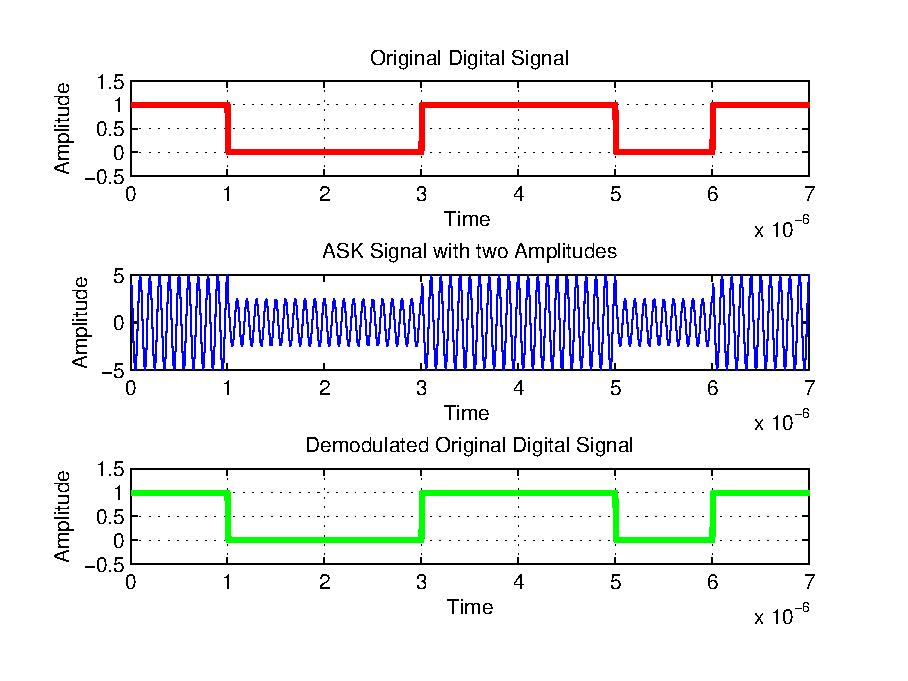
\includegraphics[width=0.7\textwidth]{ASKexample.eps}
    \caption[ASK modulation example]{ASK modulation example in the absence of noise for amplitudes $a_1=2.5$ and $a_2=5$.}
    \label{fig:ask}
\end{figure}

It is important to have an high signal-to-noise ratio (SNR), especially when the amplitudes are close so that, the demodulator is able to identify them. The ASK scheme is very sensitive to atmospheric noise, distortions and propagation conditions.  A possible demodulator is shown in figure \ref{fig:askdem}.

\begin{figure}[h]
  \centering
    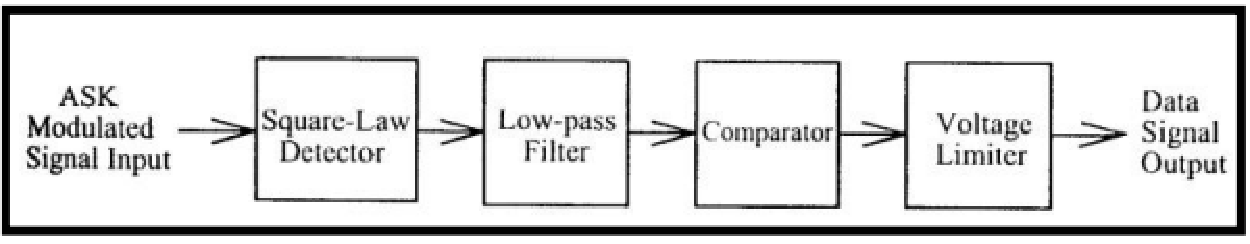
\includegraphics[width=0.7\textwidth]{askdem.pdf}
    \caption[Possible demodulator for ASK]{Possible demodulator for ASK \cite{ASKDemGaza}.}
    \label{fig:askdem}
\end{figure}


\subsection{PSK}

Phase-shift keying (PSK) is a digital modulation scheme that conveys data by changing, or modulating, the phase of a carrier wave. A finite number of phases are assigned to an unique pattern of binary digits. Usually, each phase encodes an even number of bits. The demodulator, which is designed specifically for the symbol-set used by the modulator, determines the phase of the received signal and maps it back to the corresponding signal. In digital phase modulation, the number of signal waveforms $M$ is represented as: 

\begin{equation}\label{Eq:PSK symbol}
\begin{array}{*{20}{c}}
{{s_i}(t) = }&{A\cos ({\omega _c}t + {\phi _i}(t)) = \overbrace {A\cos ({\phi _i}(t))}^{in - phase\;{\rm{symbol}}\;{{\rm{x}}_i}(t)} \cdot \cos ({\omega _c}t) \underbrace {-A\sin ({\phi _i}(t))}_{quadrature\;{\rm{symbol}}\;{{\rm{x}}_q}(t)} \cdot \sin ({\omega _c}t)}\\
{}&{ = {x_i}(t)\cos ({\omega _c}t) + {x_q}(t)\sin ({\omega _c}t)} \ ,
\end{array}
\end{equation}
where $A$ is the amplitude of the signal and ${\omega _c}$ is the carrier frequency in radians per second. An example of the decision regions for a M-PSK scheme is depicted in figure \ref{fig:pskdr}.

  
 Alternatively, instead of using the bit allocation to set the carrier's phase it can be used to change the phase by a given angle. Therefore, the demodulator determines the changes in the phase of the received signal, rather than the phase. Since this scheme depends on the difference between successive phases it is called differential phase-shift keying (D-PSK). 

 \begin{figure}[H]
  \centering
    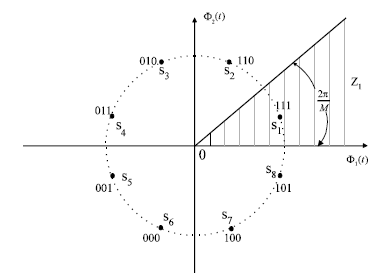
\includegraphics[width=0.4\textwidth]{PSKmodulation.png}
    \caption[Decision regions for 8-PSK]{Decision regions for 8-PSK. The minimum distance between symbols is given by $d_{min}=A\sin\frac{2\pi}{M}$  \cite{XiongDigModTech}.}
    \label{fig:pskdr}
\end{figure}


One of the advantages of PSK/D-PSK is that it is more bandwidth efficient compared to the FSK scheme. However, the signal detection/recovery is much harder compared to ASK and FSK. This is because the demodulator must determine the phase of received sinusoid with respect to some reference phase. Additionally, if a higher rate PSK scheme is used, the equipment must be capable of distinguishing small differences in phase, making it unusable in time-varying channels.

\subsection{FSK}
\label{subsec:fsk}
Frequency shift keying (FSK) is a modulation technique in which data is transmitted through discrete frequency changes of a carrier wave with fixed amplitude $A$.  In figure \ref{fig:fskex} the simplest form of FSK (e.g. binary FSK or BFSK) is illustrated. A sinusoid carrier $s_i(t)$ is transmitted for each bit, zero or one, using the carrier frequencies $f_0$ and $f_1$, respectively. 

\begin{figure}[H]
  \centering
    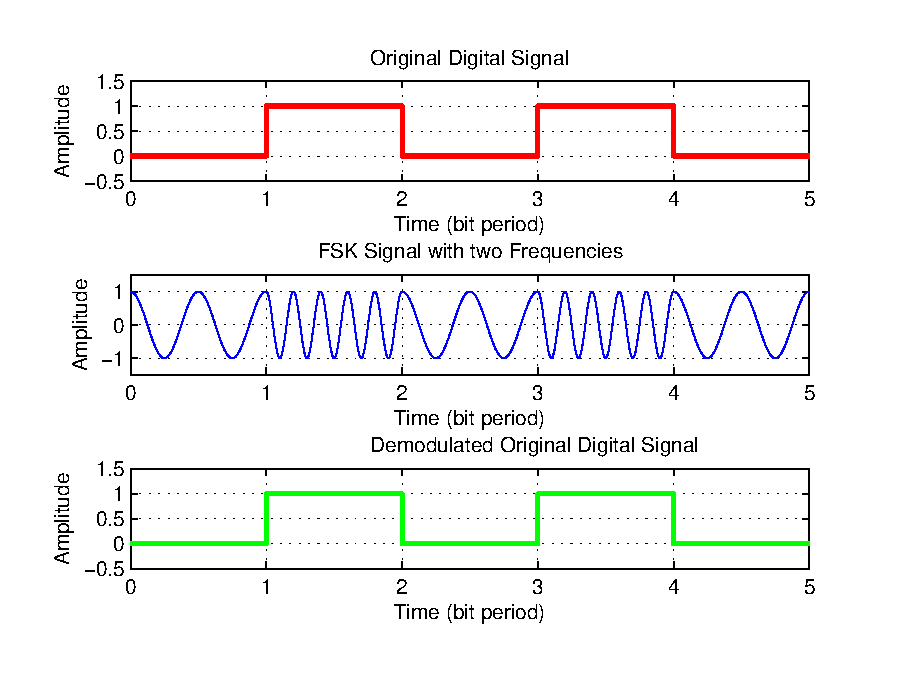
\includegraphics[width=0.7\textwidth]{fskexample.eps}
    \caption[BFSK example]{BFSK example for 2 low frequency carriers.}
    \label{fig:fskex}
\end{figure}

We can use multiple carriers to transmit $n>1$ bits. In order to guarantee that the symbols are orthogonal, there should be a $\Delta f=\frac{k}{2T}$ separation among the  $M=2^n$ carrier frequencies, where $k$ is an integer and $T$ is the bit period. The complex baseband signalling waveforms for M-ary FSK \cite{Madhow} are given in the following equation:

\begin{equation}\label{Eq:M-FSK symbols}
{s_i}(t) = {e^{j2\pi {f_i}t}}{I_{[0,T]}},i = 1,2,...,M
\end{equation}



Coherent and non-coherent demodulation methods exist and depend on whether the phase of the sinusoids $\phi$ are equal or not. Coherent demodulators consist of correlators (matched filters) and samples, but they require synchronisation of the reference signals. The demodulator for BFSK can be implemented with two correlators as shown in figure \ref{fig:FSKdemcoherent}. This receiver is optimum in the sense that it minimizes the error probability for equally-likely binary signals. If for example a sinusoid carrier with frequency $f_1$ is transmitted, the upper correlator yields a signal $l_1$ with a positive signal component, while $l_2$ has only a noise component. This is due to orthogonality of the signals.
  In case there is no phase reference, additional squarers or envelope detectors must be used for the non-coherent detection. In the last case, a minimum tone spacing of $\frac{k}{T}$ is required instead. The correlator implementation for non-coherent BFSK is illustrated in figure (\ref{fig:FSKdemNoncoherent}).

 \begin{figure}[H]
 \centering
\begin{subfigure}[h]{0.9\textwidth}
 \centering
    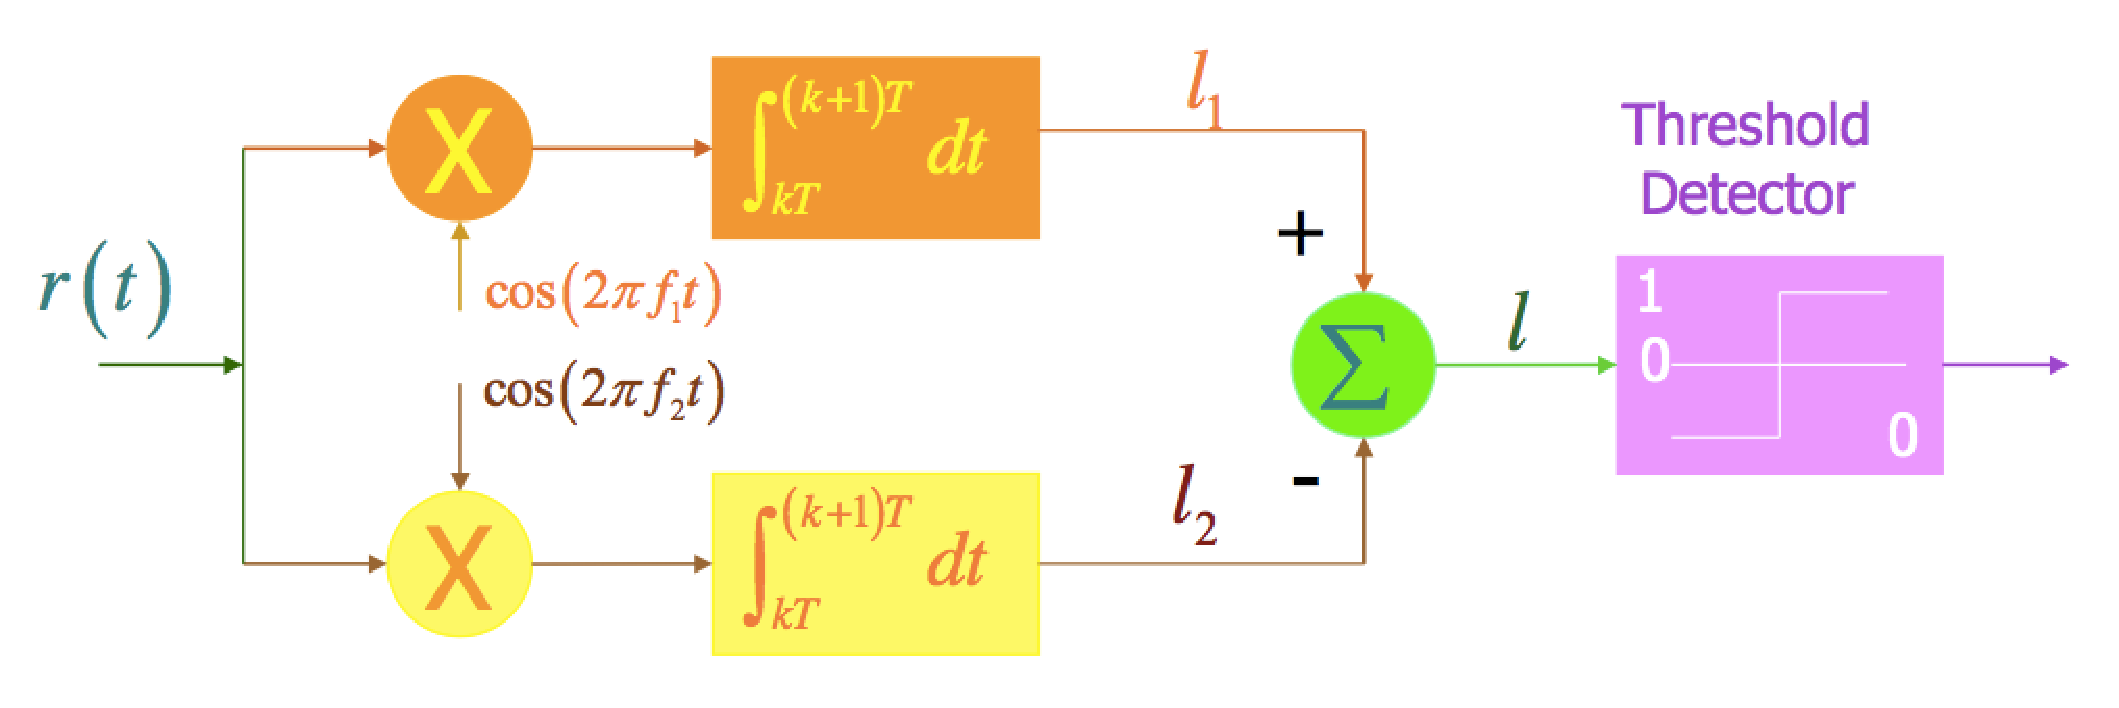
\includegraphics[width=0.6\textwidth]{fskdem1.pdf}
    \subcaption{Coherent.}
    \label{fig:FSKdemcoherent}

\end{subfigure}
\quad

\begin{subfigure}[H]{0.9\textwidth}
 \centering
    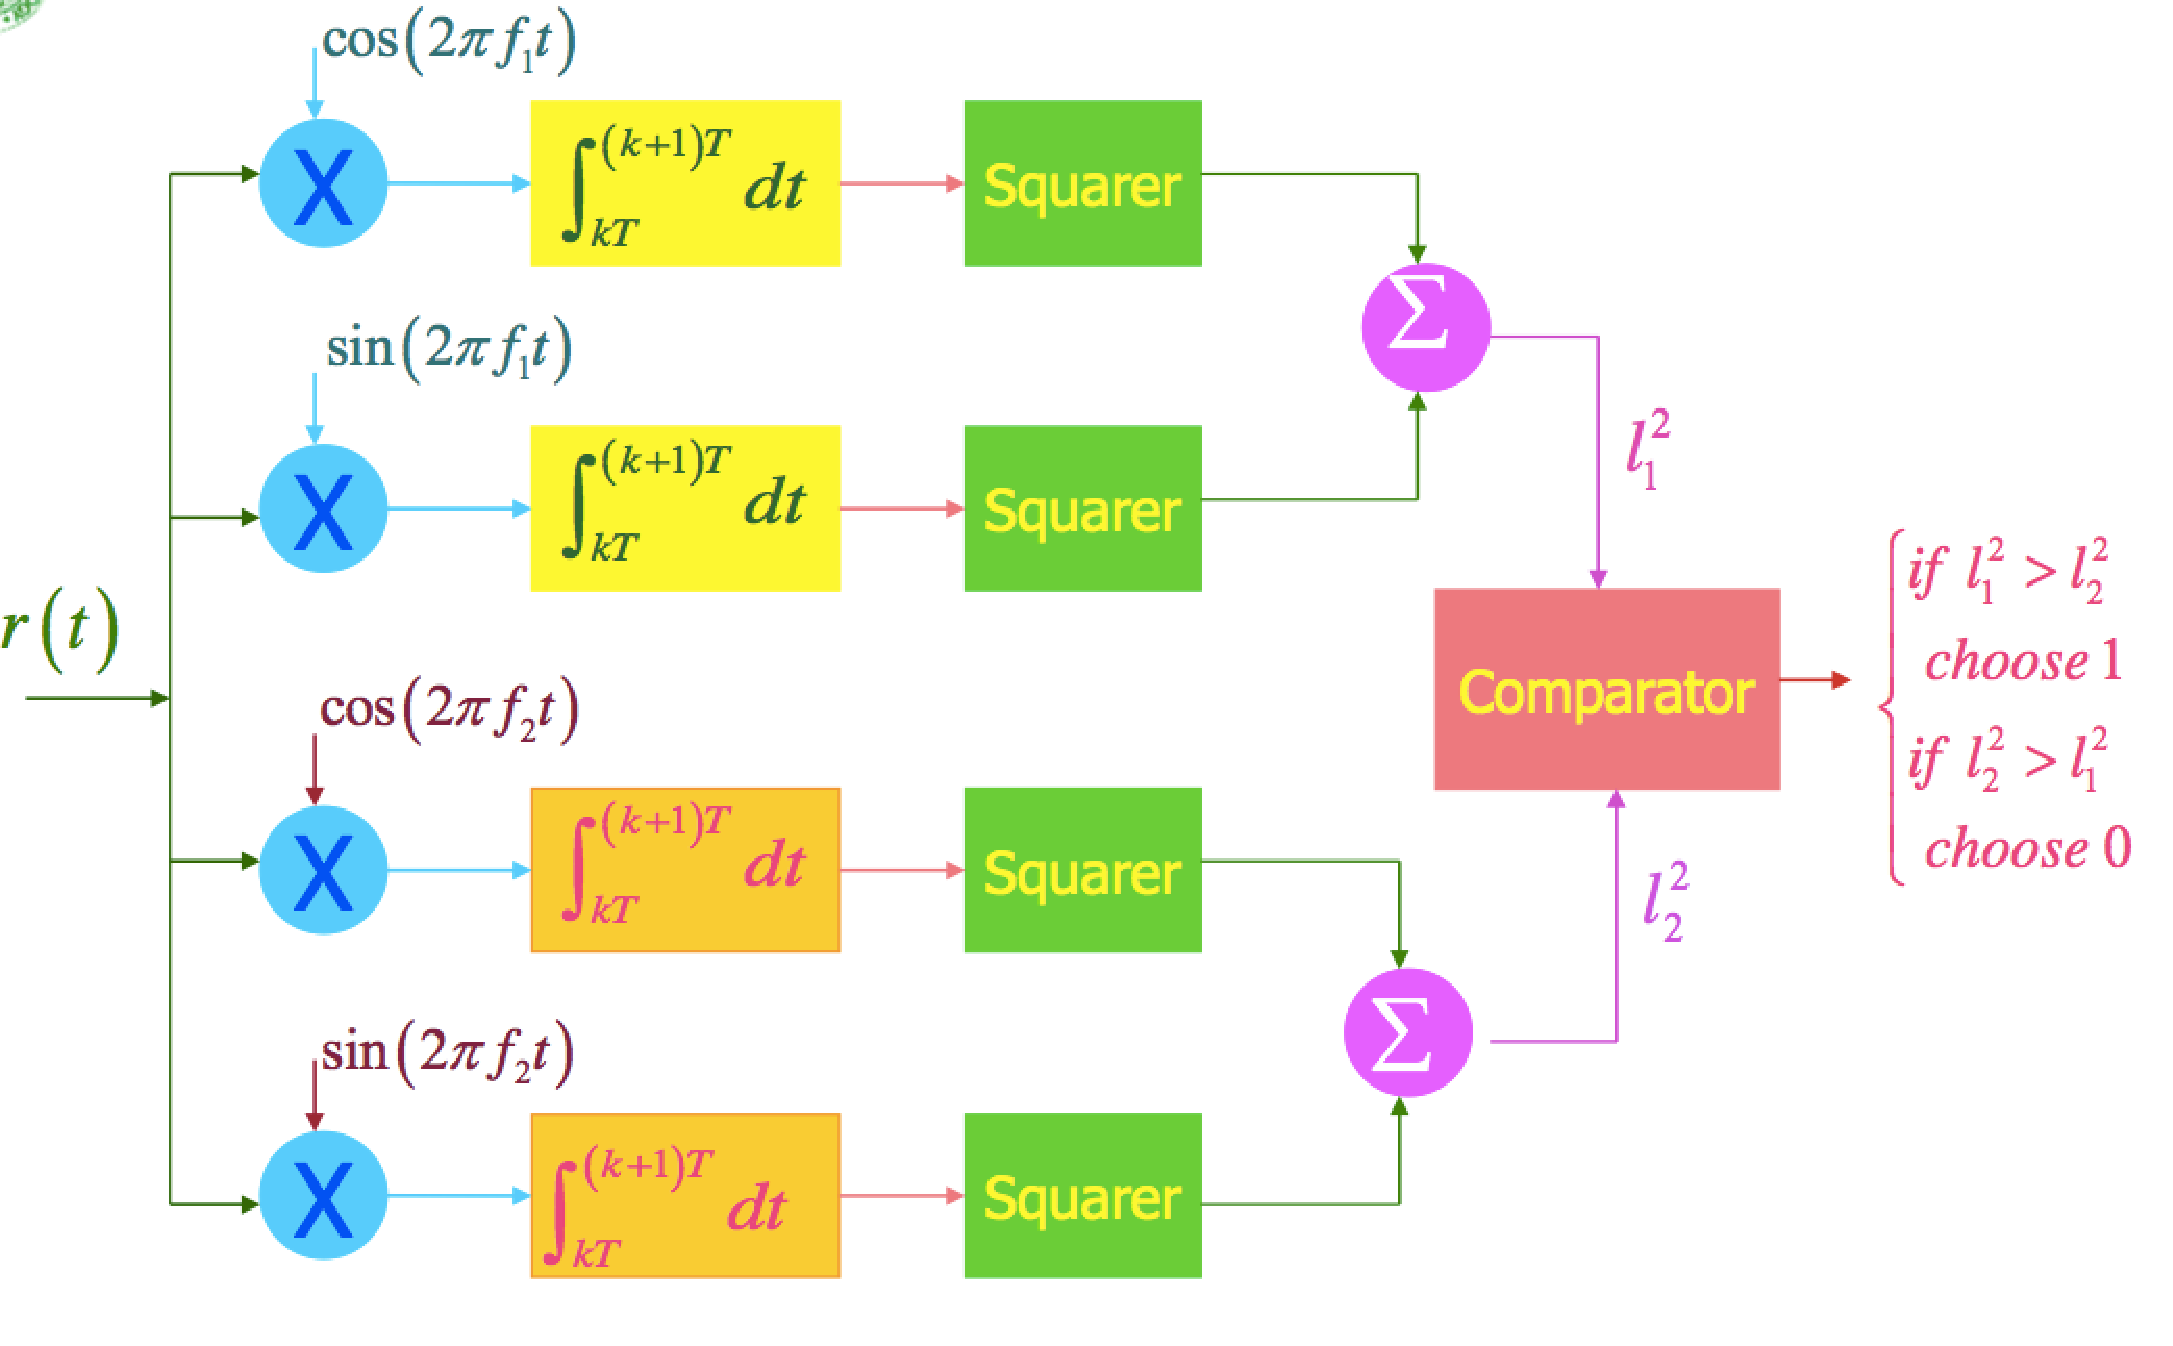
\includegraphics[width=0.6\textwidth]{fskdem2.pdf}
    \subcaption{Non-coherent.}
    \label{fig:FSKdemNoncoherent}
    \end{subfigure}
    \caption[Possible demodulators for FSK]{Possible demodulators for FSK \cite{DigModTech}.}
\end{figure}


It is expected that the error performance for the non-coherent receivers is greater than the coherent ones. However, the degradation is only a fraction of a decibel. Other options for demodulation are available, such as the use of FFT schemes for peak picking or bandpass filtering at the working frequencies.

 \subsubsection{Performance}
 
 FSK systems have the higher power efficiencies among the available modulation schemes but they suffer from the low bandwidth (BW) efficiency. The main advantages of this modulating scheme are: the in-sensitiveness to amplitude variations in the channel, its compatibility with non-linear transmitters and receivers, and the fact that it is not required to have an absolute frequency accuracy for correct demodulation\footnote{FSK is tolerant to local oscillator drifts and Doppler shifts.}. One of the drawbacks is the fact that it is less bandwidth efficient when compared with other schemes such as ASK or PSK. To avoid undesirable spectral characteristics\footnote{Spectral leakage could cause adjacent channel interference.}, continuous phase FSK is required (see figure \ref{fig:comparecpfsk} for comparison).
%
 \begin{figure}[H]
 \centering
	\begin{subfigure}[H]{0.9\textwidth}
 \centering
    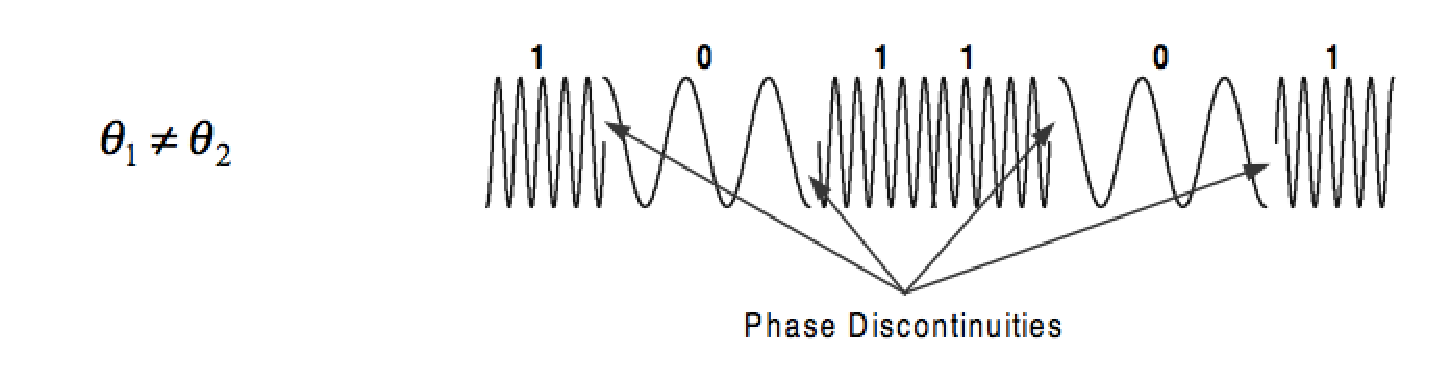
\includegraphics[width=0.6\textwidth]{ncpfsk.pdf}
    \subcaption{Non continuous phase FSK.}
    \label{fig:FSKcoherent}

	\end{subfigure}
	\quad

	\begin{subfigure}[H]{0.9\textwidth}
 	\centering
    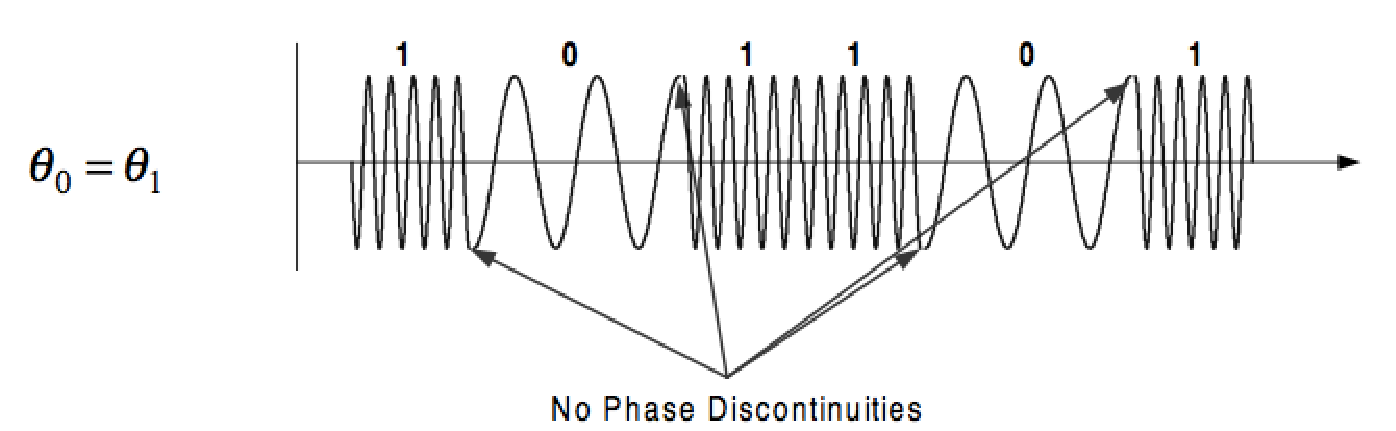
\includegraphics[width=0.6\textwidth]{cpfsk.pdf}
    \subcaption{Continuous phase FSK.}
    \label{fig:FSKnoncoherent}
 	\end{subfigure}
    \caption[Effects of phase discontinuity in FSK signal]{Effects of phase discontinuity in FSK signal in time domain \cite{DigCommLec}.}
    \label{fig:comparecpfsk}
\end{figure}

The M-ary FSK modulated signals can be written as follows:

\begin{equation}\label{Eq:M-FSK symbol 2}
{s_m}(t) = A{\varphi _m}(t),\quad 0 \le t \le T_s
\end{equation}

We can read $T_s$, from equation \ref{Eq:M-FSK symbol 2}, as the period of the input symbol stream, and $A$ as the amplitude of the basis function $\varphi_m$. In addition, the basis functions can be described by:

\begin{equation}\label{Eq:M-FSK basis}
{\varphi _m}(t) = \sqrt {\frac{2}{T}} \cos \left( {2\pi ({f_c} + {\alpha _m}\Delta {f_c}) + {\theta _m}} \right), \quad 0 \le t \le T
\end{equation}

where \[
{\alpha _m} \in \left\{ {(2m - 1 - M) | m = 1,2,...,M} \right\}
\] 
In order to satisfy orthogonality, the inner product between the basis functions must be one for $m=n$, and zero for $m\neq n$:
\begin{equation}\label{Eq:M-FSK inner product}
\left\langle {\left. {{\varphi _m},{\varphi _n}} \right\rangle } \right. = \int {{\varphi _m}(t)\cdot {\varphi _n}(t)dt = {\delta _{mn}} = \left\{ \begin{array}{l}
1\text{, }m = n\\
0\text{, }m \ne n
\end{array} \right.}
\end{equation} 


Individual frequencies corresponding to different symbols are given by equation \ref{Eq:M-FSK fm}, where $f_c$ is the central frequency and $\Delta f_c$ is the frequency separation.\\
\begin{equation}\label{Eq:M-FSK fm}
{f_m} = {f_c} + {\alpha _m}\Delta {f_c}
\end{equation}
Thus, equation \ref{Eq:M-FSK deltaF} must apply to satisfy orthogonality (see \cite{gold}):

\begin{equation}\label{Eq:M-FSK deltaF}
\Delta {f}= 2\Delta {f_c} = \left\{ \begin{array}{l}
\frac{1}{{2T}}, \quad {\theta _m} = {\theta _n}, \quad \forall\text{ } m,n\\
\frac{1}{T}, \quad {\theta _m} \ne {\theta _n}
\end{array} \right.
\end{equation}

The overall bandwidth occupied by the FSK signal depends on the modulation index $h$ described in equation \ref{Eq:M-FSK mod index}.
\begin{equation}\label{Eq:M-FSK mod index}
h=\frac{2\Delta {f_c}}{R}=2\Delta {f_c}T_s 
\end{equation}

For continuous phase BFSK the minimum value for the signals to not interfere with each other is $h=0.5$. A FSK system using continuous phase transitions has much lower sidelobe energy than the discontinuous case. All these parameters will cause inter-symbol-interference (ISI) and limit the rate of the system. For this reason it is important to further increase the bandwidth efficiency of the system by applying pulse shaping to the transmitted signal. This technique is described in section \ref{Sec:Pulse shaping}. 



\subsection{M-QAM}
M-ary Quadrature-Amplitude modulation is a two-dimensional signalling scheme that combines both Amplitude and Phase Shift Keying. The transmitted signal for every symbol can be written as \cite{Proakis}:
\begin{equation}\label{Eq: MQAM symbols}
{s_i}\left( t \right) = \sqrt {\frac{{2{E_0}}}{T}} {a_i}\cos \left( {2\pi {f_c}t} \right) - \sqrt {\frac{{2{E_0}}}{T}} {b_i}\sin\left( {2\pi {f_c}t} \right), \quad \left\{ {\begin{array}{*{20}{c}}
{0 \le t \le T}\\
{i = 0, \pm 1, \pm 2, \ldots }
\end{array}} \right.
\end{equation}

The typical in phase (I) and quadrature (Q) known as IQ modulation and demodulation is shown in figure \ref{fig:iqmodem}. We consider that the information to be transmitted is a complex signal $x=x_i+jx_q$. Ignoring the energy and period factors, the output of the IQ modulation transmitter is given by \cite{Madhow}:

\begin{equation}\label{EQ: MQAM IQ}
y(t) = \Re \{ x{e^{j2\pi {f_c}t}}\}  = {x_i}\cos (2\pi {f_c}t) - {x_q}\sin (2\pi {f_c}t)
\end{equation}

 \begin{figure}[H]
  \centering
    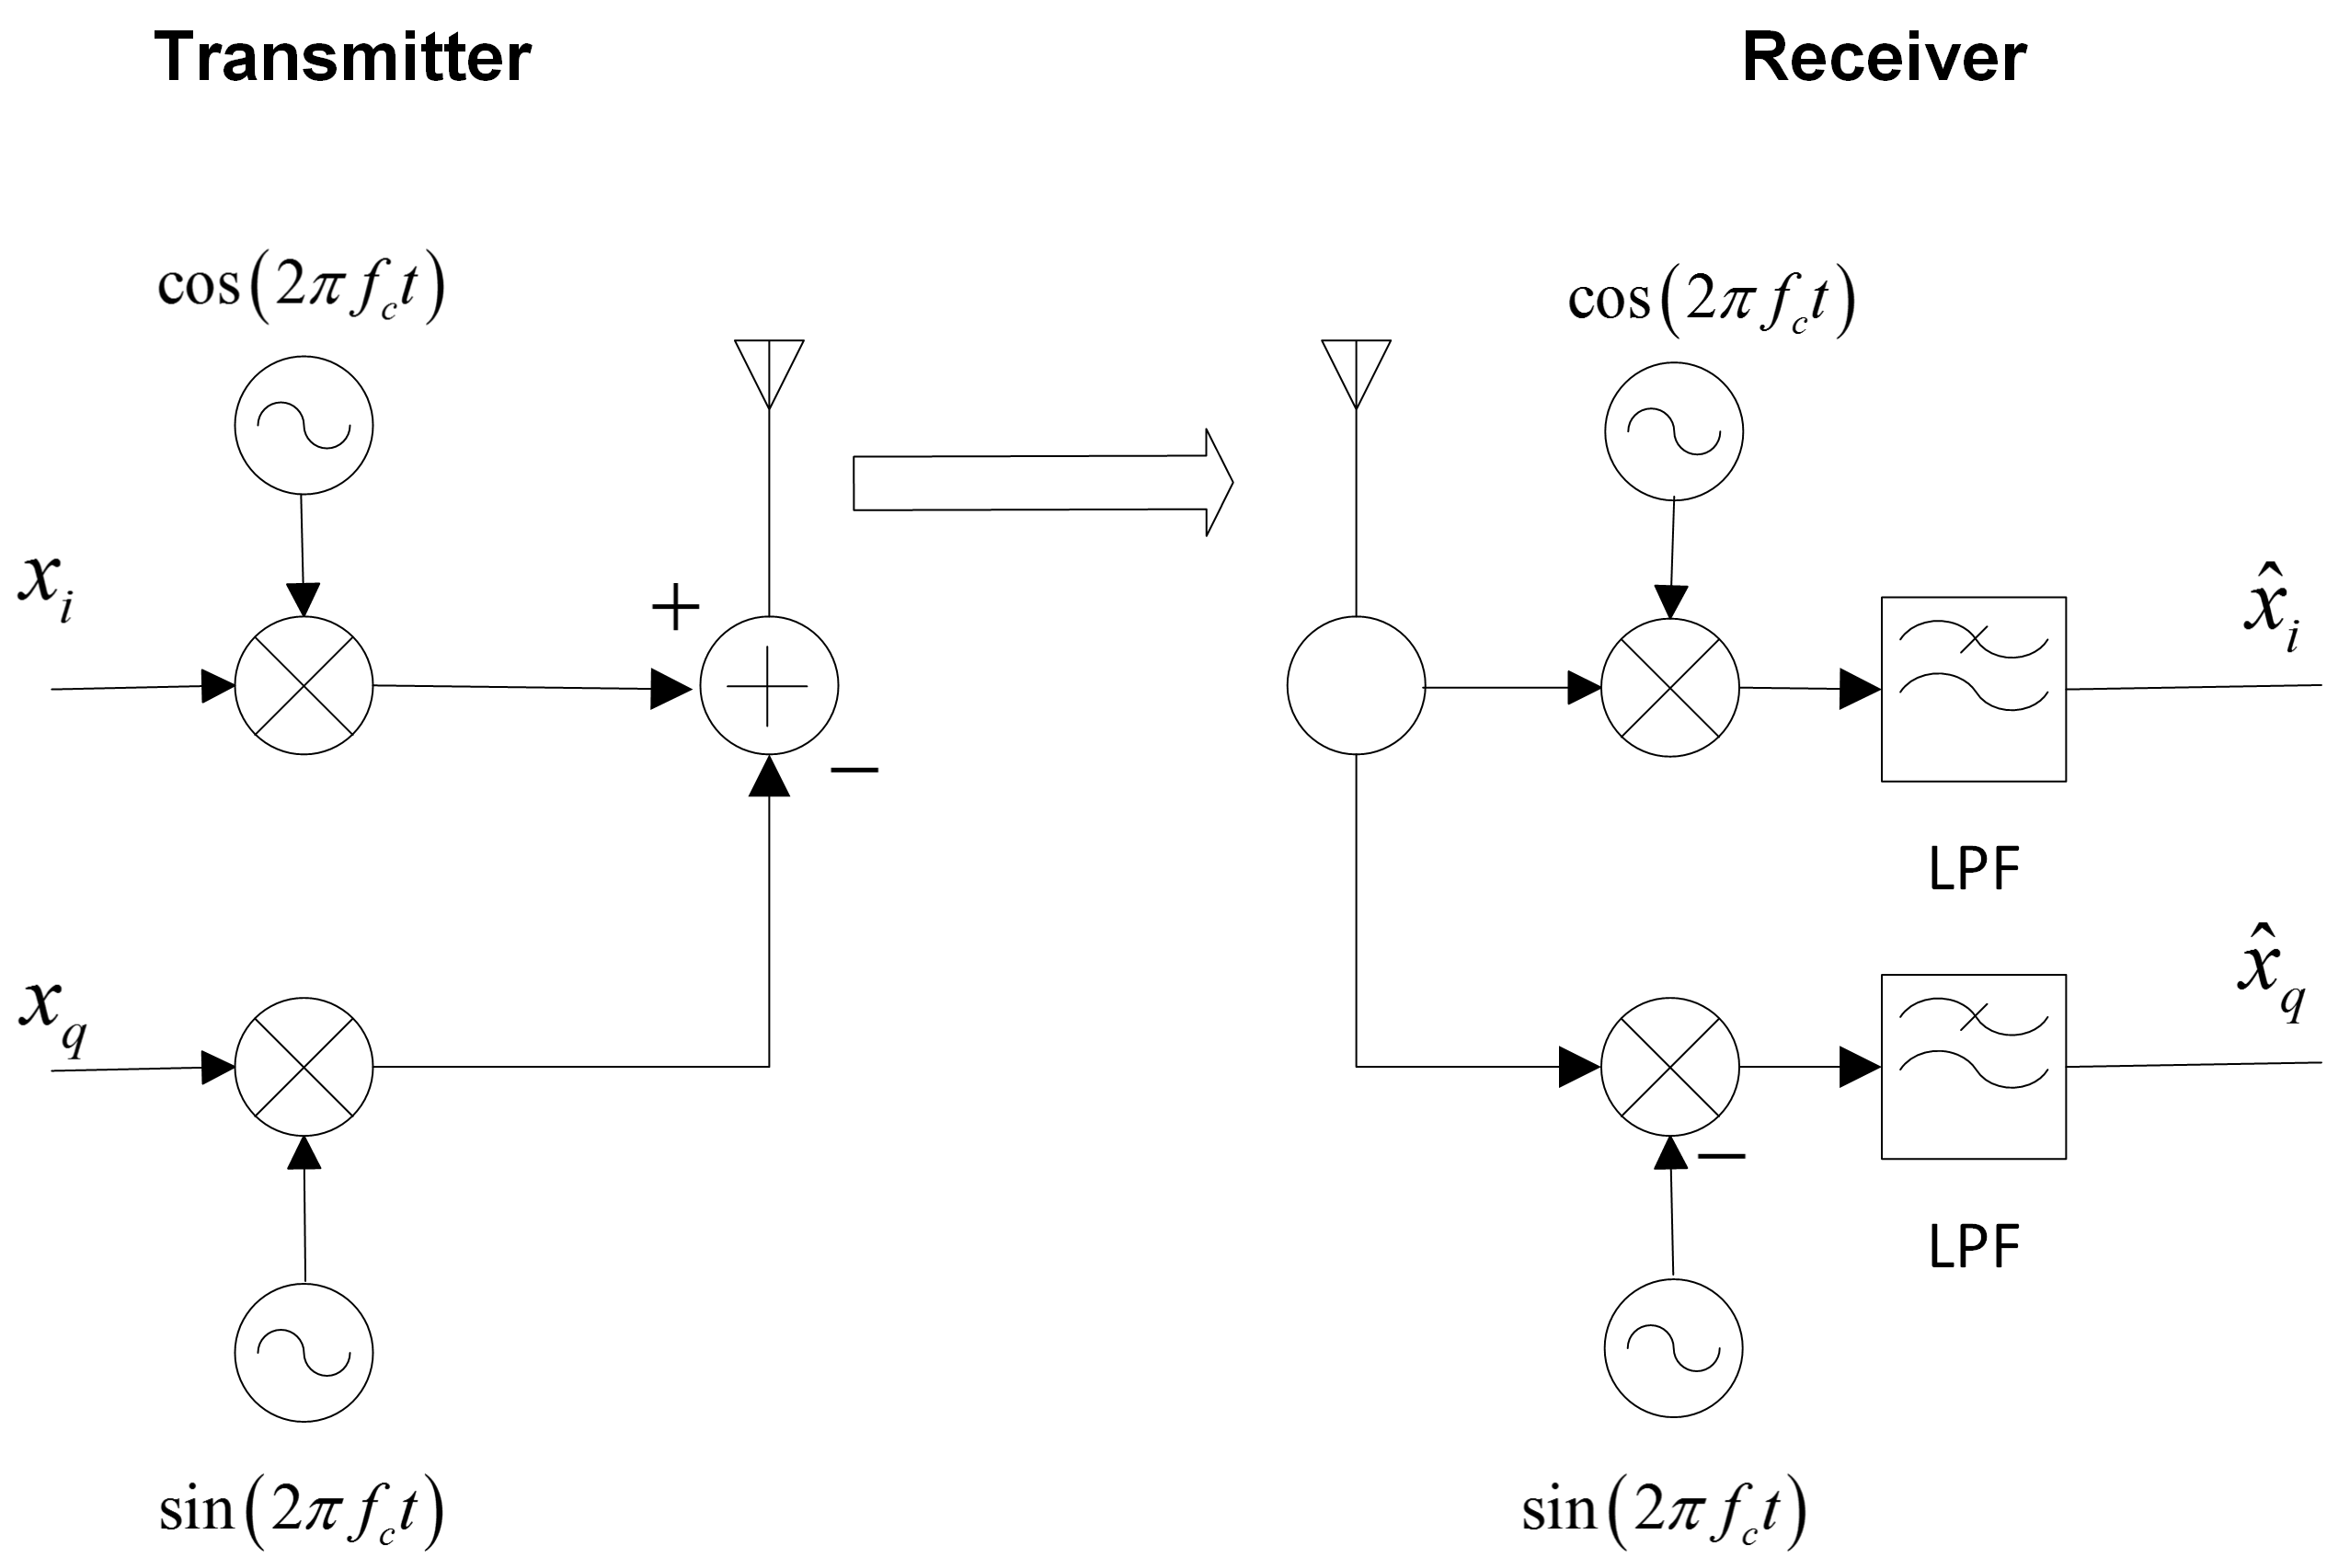
\includegraphics[width=0.7\textwidth]{MQAMsyst.png}
    \caption[Schematic of M-QAM transmitter and receiver]{Schematic of M-QAM transmitter and receiver showing the in-phase ($x_i$) and quadrature components ($x_q$).}
    \label{fig:iqmodem}
\end{figure}



At the transmitter, the signal $x_i$ is mapped to $\cos (2\pi {f_c}t)$ and $x_q$ is mapped to $\sin (2\pi {f_c}t)$. At the receiver, we multiply the signal with $\cos (2\pi {f_c}t)$ and $\sin (2\pi {f_c}t)$ carriers\footnote{Note the minus sign in the sinus component shown in figure \ref{fig:iqmodem}.}, followed by low-pass filtering to extract $\hat{x}_i$ and $\hat{x}_q$. The mathematical expressions for the recovered information at the receiver, using the trigonometric identities, can be summarized as follows \cite{Madhow}: 

\begin{eqnarray}
{{\hat x}_i} = \int\limits_0^T {y \cdot \cos (2\pi {f_c}t)dt = } \int\limits_0^T {\left( {{x_i}\cos (2\pi {f_c}t) - {x_q}\sin (2\pi {f_c}t)} \right) \cdot \cos (2\pi {f_c}t)dt\mathop  = \limits^{LPF} \frac{{{x_i}}}{2}}\\
{{\hat x}_q} = \int\limits_0^T { - y\cdot \sin (2\pi {f_c}t)dt = } \int\limits_0^T { - \left( {{x_i}\cos (2\pi {f_c}t) - {x_q}\sin (2\pi {f_c}t)} \right) \cdot \sin (2\pi {f_c}t)dt\mathop  = \limits^{LPF} \frac{{{x_q}}}{2}} 
\end{eqnarray}

By ignoring the scaling factor of $\frac{1}{2}$ and assuming that the channel is ideal, both $x_i$ and $x_q$ can be recovered successfully. 

\subsubsection{QAM Symbol Mapping}

As stated previously, the QAM scheme involves sending digital information by periodically adjusting the phase and amplitudes of a sinusoidal wave. For example, 4-QAM consists of four unique combinations of phase and amplitude. These combinations, called symbols, are shown as the white dots on the constellation plot in figure \ref{fig:4qamsym}. It is possible to send up to two bits per symbol when using 4-QAM modulation. It is also possible to send data at even higher rates by increasing the number of symbols in our symbol map. By convention, the number of symbols in a symbol map is called the symbol map “M” and is considered the “M-ary” of the modulation scheme. The number of bits in an M-QAM scheme is given by ${{{\log }_2}M}$. 


 \begin{figure}[H]
  \centering
    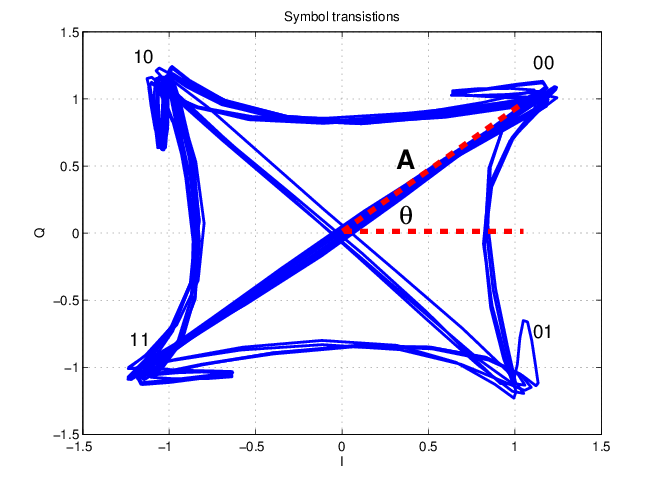
\includegraphics[width=0.7\textwidth]{4symboltransitions.png}
    \caption[Symbol transitions in 4-QAM]{Symbol transitions in 4-QAM. The blue lines represent the phase and amplitude transitions from one symbol to another. Labelled in the constellation plot, there is the digital bit pattern that each symbol represents.}
    \label{fig:4qamsym}
\end{figure}



\subsubsection{M-QAM Impairments}
Although QAM appears to increase the transmission efficiency for digital communication systems by utilising both amplitude and phase variations, it has a number of drawbacks. It is more susceptible to noise because the states are closer together. This means a lower level of noise is needed to move the signal to a different decision point. The second limitation is that linearity must be maintained when the signal is passed through the channel and amplifiers. Both these limitations are associated with the amplitude component of the signal. 

In an ideal IQ modulator, the phase difference between the signals used for modulating the I and Q arm is 90 degrees, resulting in using $\cos (2\pi {f_c}t)$ and $\sin (2\pi {f_c}t)$ for sending $x_i$ and $x_q$, respectively. If there is phase imbalance, the phase difference might not be exactly 90 degrees. In that case, we can consider that $\cos (2\pi {f_c}t)$ and $\sin (2\pi {f_c}t + \varphi )$ carriers are used for transmitting instead.
When there is amplitude imbalance small level variations will be added in the sine and cosine carriers at the modulator. This can be modelled by using $\cos (2\pi {f_c}t)$ for the in-phase component $x_i$, and  $(1 + \alpha )\sin (2\pi {f_c}t)$ to carry the quadrature component $x_q$.

The transmitted signal including the effect of phase and amplitude imbalance is then \cite{Madhow}:
\begin{equation}\label{eq:MQAMimpairedRcvdSignal}
y(t) = {x_i}\cos (2\pi {f_c}t) - {x_q}(1 + \alpha )\sin (2\pi {f_c}t + \varphi ) \text{,\quad where }0 < \alpha < 1
\end{equation}

Assuming that we have an ideal IQ demodulator at the receiver, we split in two the received signal $y(t)$ and multiply one of the resultant with a $\cos (2\pi {f_c}t)$ carrier and the other with a $\sin (2\pi {f_c}t)$ carrier. The outcome of such multiplications is low-pass filtered, allowing to extract  $\hat{x}_i$ and $\hat{x}_q$ respectively for every branch:
\begin{eqnarray}
{{\hat x}_i} & = & \frac{1}{2}\left[ {{x_i} - {x_q}(1 + \alpha )\sin (\varphi )} \right]\\
{{\hat x}_q} & = & \frac{1}{2}\left[ {{x_q}(1 + \alpha )\cos (\varphi )} \right]
\end{eqnarray}

These non-idealities leads to a quadrature skew that causes a different mapping in both the transmitter and receiver. IQ gain imbalance equates to a rectangular stretch along the IQ axis. Likewise, quadrature error results in the IQ axis not being exactly $90\degree$ apart. These phenomena can be seen in figure \ref{fig:skewed}.


\begin{figure}[H]
 \centering
	\begin{subfigure}[H]{0.9\textwidth}
 	\centering
    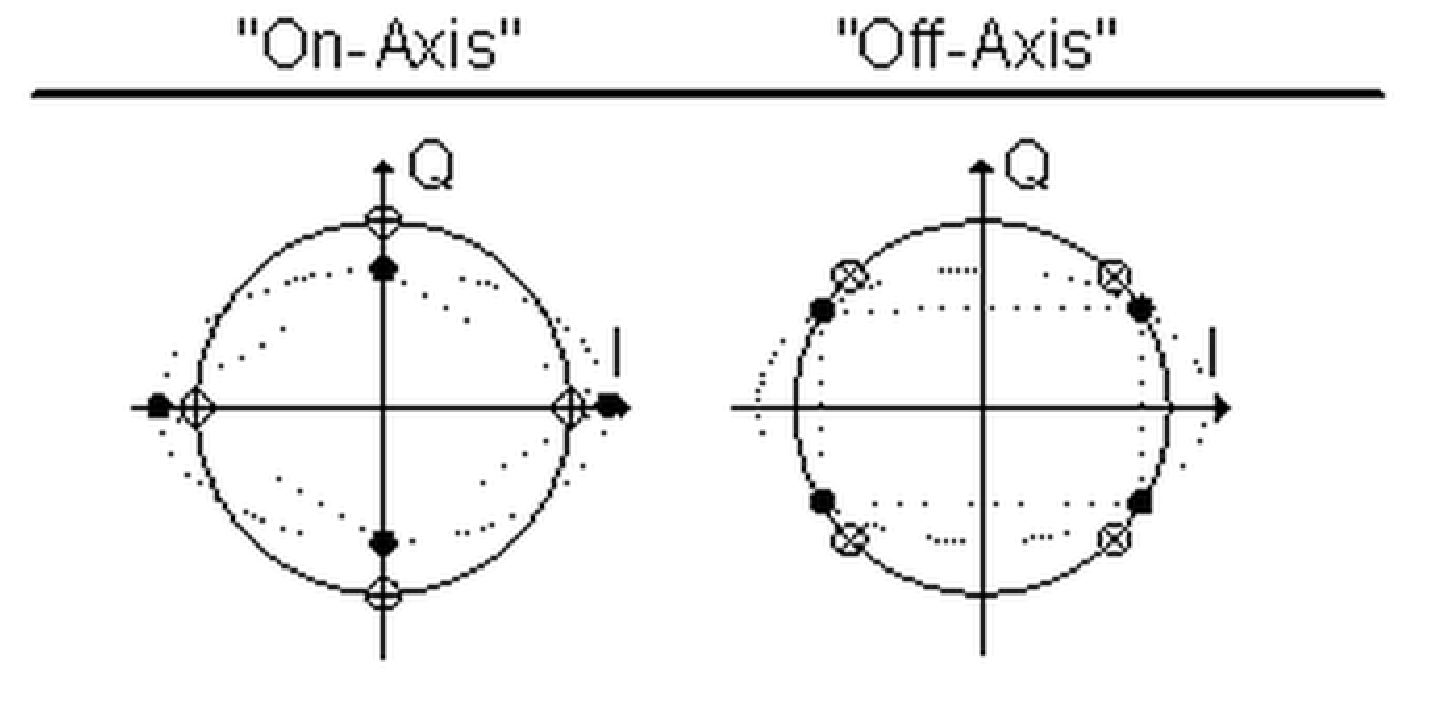
\includegraphics[width=0.6\textwidth]{gi.pdf}
    \subcaption{IQ gain imbalance.}
    %%\label{}

	\end{subfigure}
	
	\begin{subfigure}[H]{0.9\textwidth}
 	\centering
    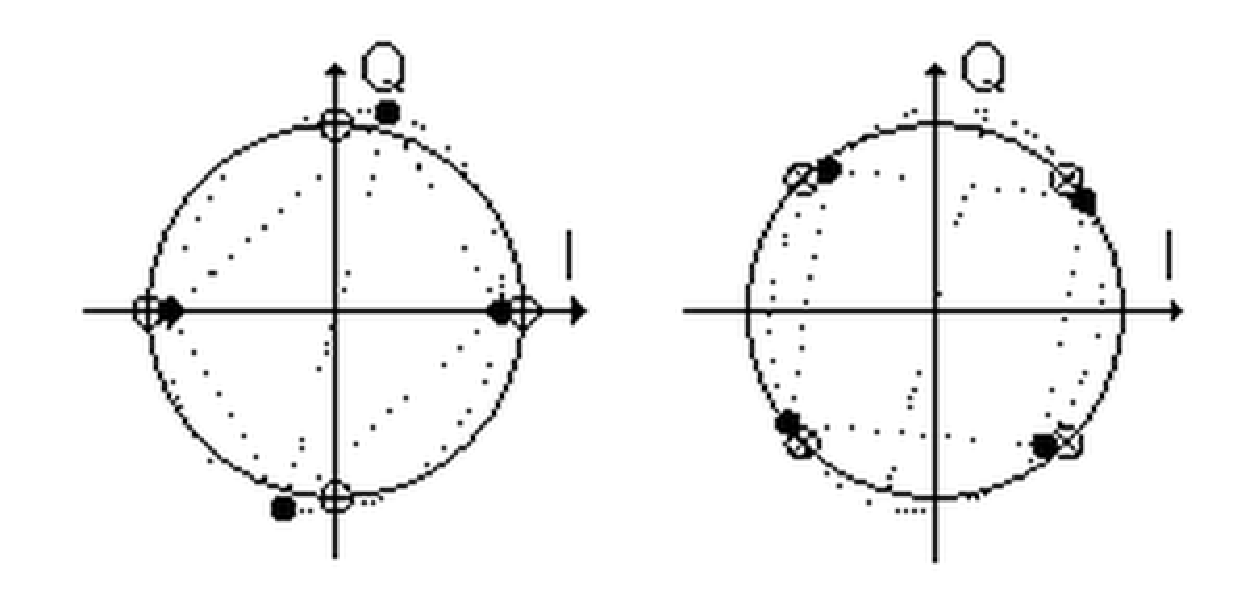
\includegraphics[width=0.5\textwidth]{qe.pdf}
    \subcaption{IQ quadrature error.}
   %% \label{}
 	\end{subfigure}
    \caption[Two possible constellation mappings for 4-QAM]{Two possible constellation mappings for 4-QAM and the effects of impairments on phase and amplitude \cite{Agilent IQ paper}.}
    \label{fig:skewed}
\end{figure}


\subsubsection{Performance and Impact of Noise}
\label{sec:MQAMperf}
When studying the impact of the noise in QAM systems we assume that Gray coding is used, all symbols are equiprobable, the noise is zero-mean additive white Gaussian noise (AWGN) with variance $\frac{N_0}{2}$ and there are no errors from carrier recovery or symbol synchronisation. In a square M-QAM system the amplitudes of $x_i$ and $x_q$ can take $\log_2{M}$ different values. Each level can be 
$ -(\sqrt M  -1)\cdot d, - (\sqrt M  - 3)\cdot d,\cdots,(\sqrt M  - 1)\cdot d $, where $d$ is half of the minimum distance between two symbols. The value of $d$ can be computed as \cite{BER-QAM paper}: 
\begin{equation}\label{Eq: MQAM min dist}
d = \sqrt {\frac{{3{{\log }_2}(M) \cdot {E_b}}}{{2(M - 1)}}}\ ,
\end{equation}
where $E_b$ is the energy per bit in the transmitter. Recall that at the demodulator, the received vector is given by \cite{BER-QAM paper}: 
\begin{equation}
 \mathbf{r}=\mathbf{s}+\mathbf{n}=\left[ \begin{array}{l}I\\Q \end{array} \right] + \left[ \begin{array}{l}{n_i}\\{n_q}\end{array} \right]\ ,
\end{equation}


The proof of the BER expression for the MQAM is out of the scope of this report. However the final generic result is given as: 
\begin{equation}\label{Eq: BER MQAM}
{P_b} = \frac{1}{{{{\log }_2}\sqrt M }}\sum\limits_{k = 1}^{{{\log }_2}\sqrt M } {{P_b}(k)}\ ,
\end{equation}


The conditional BER,  $P_b(k)$ in equation \ref{Eq: BER MQAM}, corresponding to the k-th bits $(k=1,2,3,... \log_2{\sqrt{M}} )$ on both I and Q components is defined as follows \cite{BER-QAM paper}:
\begin{equation} \label{eq:mqamBER}
{P_b}(k) = \frac{1}{{\sqrt M }}\sum\limits_{j = 0}^{(1 - {2^{ - k}})\sqrt M  - 1} {\left[ {{{( - 1)}^{\left\lfloor {\frac{{j{2^{k - 1}}}}{{\sqrt M }}} \right\rfloor }}\left( {{2^{k - 1}} - \left\lfloor {\frac{{j{2^{k - 1}}}}{{\sqrt M }} + \frac{1}{2}} \right\rfloor } \right) \cdot \text{erfc}\left( {(2j + 1)\sqrt {\frac{{3{{\log }_2}(M) \cdot {E_b}}}{{2(M - 1){N_0}}}} } \right)} \right]}
\end{equation}

The outcome of these expressions denoting the required $E_b / N_0$ necessary to achieve certain BER for a number of M-ary schemes is displayed in figure \ref{fig:mqamber}.

 \begin{figure}[H]
  \centering
    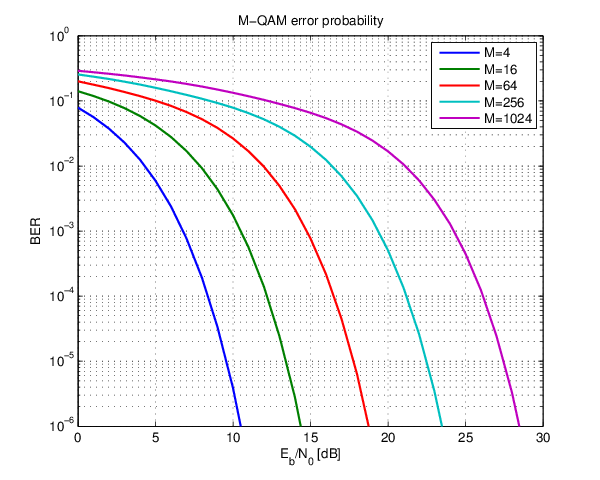
\includegraphics[width=0.5\textwidth]{MQAMber.png}
    \caption[BER Performance of M-ary QAM in function to $E_b / N_0$]{BER Performance of M-ary QAM in function to $E_b / N_0$.}
    \label{fig:mqamber}
\end{figure}




\subsection{OFDM}
\label{sec:OFDM}
OFDM or Orthogonal Frequency-Division Multiplexing, is a multi-carrier modulation scheme that divides the available bandwidth $W$ into $N$ sub-bands, with relatively narrow width $\Delta f = \frac{W}{N}$. The signal in each sub-band can be independently encoded and modulated as a synchronous symbol with rate $T = \frac{1}{\Delta f}$. If $\Delta f$ is small enough, the channel frequency response $C(f)$ is essentially constant across each sub-band. Hence, the ISI is negligible and OFDM provides a solution that could yield transmission rates close to the channel capacity. 

By choosing the modulating waveforms to be \emph{eigen-functions} of a linear-time invariant channel (LTI), it can be guaranteed that the waveforms will remain orthogonal after going through the channel. Therefore, the fact that complex exponentials $\exp{(j2\pi f_k t)}$ are orthogonal at different frequencies $f_k$  can be exploited.  Suppose that the $N$ waveforms with data to be transmitted are $X_k, k=0,1,...,N-1$, where $X_k$ is a complex number in a given constellation. If a carrier frequency $f_k$ is assigned to each symbol $X_k$ and each contribution is summed at the output, the following result is obtained:

\begin{equation}
x(t) = \sum\limits_{k = 0}^{N - 1} {{X_k}{e^{j2\pi {f_k}t}}}
\end{equation}


For the implementation of a digital system, a transmitter will generate its data output in a sampled fashion. By letting $t=nT_s$ and $f_k=k\Delta f$, with $T_s$ as the sample interval and $\Delta f$ as the sub-carrier spacing (assumed to be uniform), the output is given by:
\begin{equation}
x(n{T_s}) = \sum\limits_{k = 0}^{N - 1} {{X_k}{e^{j2\pi k\Delta fn{T_s}}}}
\end{equation}

The sub-carrier spacing should be computed such that the orthogonality of different sub-carriers holds over an interval of length $T$:

\begin{equation}
\int\limits_0^T {{e^{j2\pi {f_m}t}}{e^{ - j2\pi {f_n}t}}} dt = \frac{{{e^{j2\pi ({f_n} - {f_m})t}} - 1}}{{j2\pi ({f_n} - {f_m})}} = 0,{\text{ for }}({f_n} - {f_m})T  \in \mathbb{Z}_{\neq 0}
\end{equation}

Hence, $\Delta f = \frac{1}{NT_s}=\frac{1}{T}$ is the minimum separation to keep orthogonality among signals at different modulators, resulting in:
\begin{equation}
x(n{T_s}) = \sum\limits_{k = 0}^{N - 1} {{X_k}{e^{j2\pi kn/N}}} \text{, }n = 0,1,...,N - 1
\end{equation}


The above formula is the equation of an N-point IDFT for one OFDM symbol. If $N$ is a power of two, the samples $x(nT_s)$ can be efficiently generated (for example by using the FFT algorithm). A plot of the resulting signal in time and frequency domain is shown in figure \ref{fig:ofdmsig}.

\begin{figure}[H]
 \centering
	\begin{subfigure}[H]{0.9\textwidth}
 	\centering
    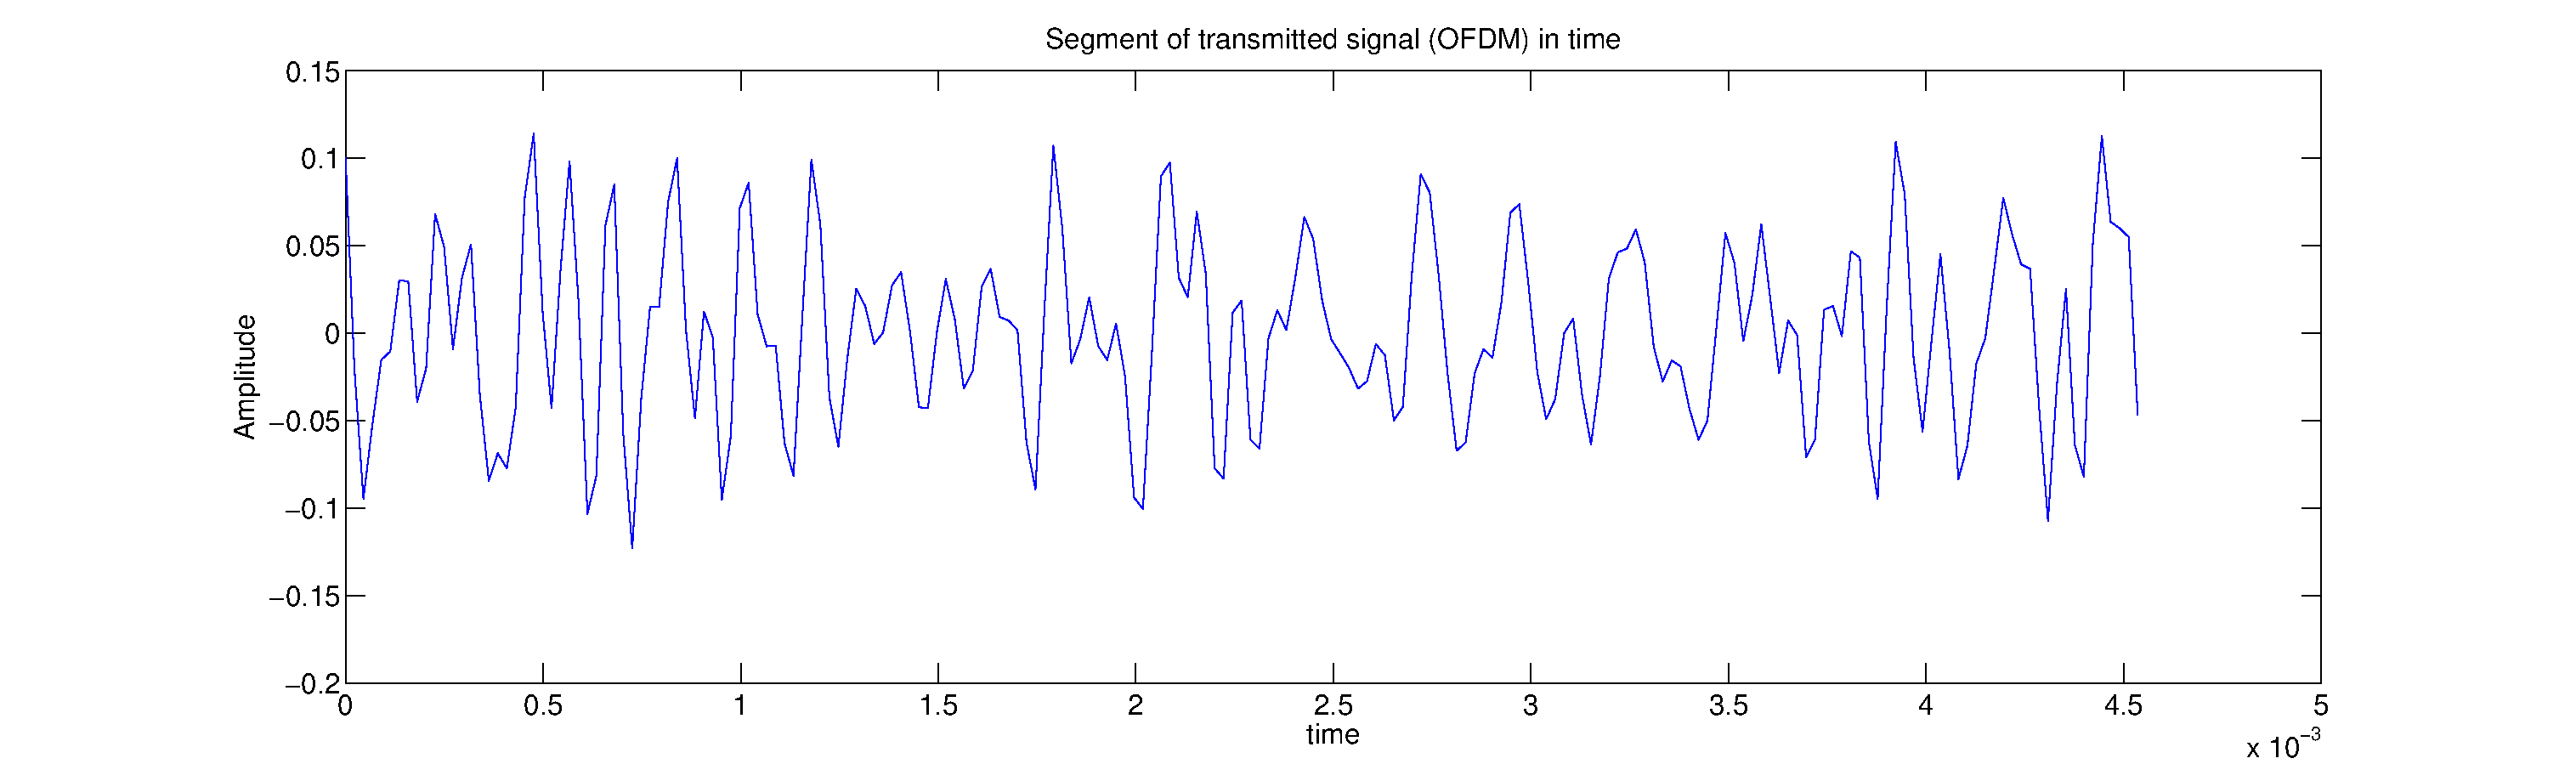
\includegraphics[width=0.9\textwidth]{ofdmsignal.eps}
    \subcaption{OFDM signal in time domain.}
    %%\label{}

	\end{subfigure}
	
	\begin{subfigure}[H]{0.9\textwidth}
 	\centering
    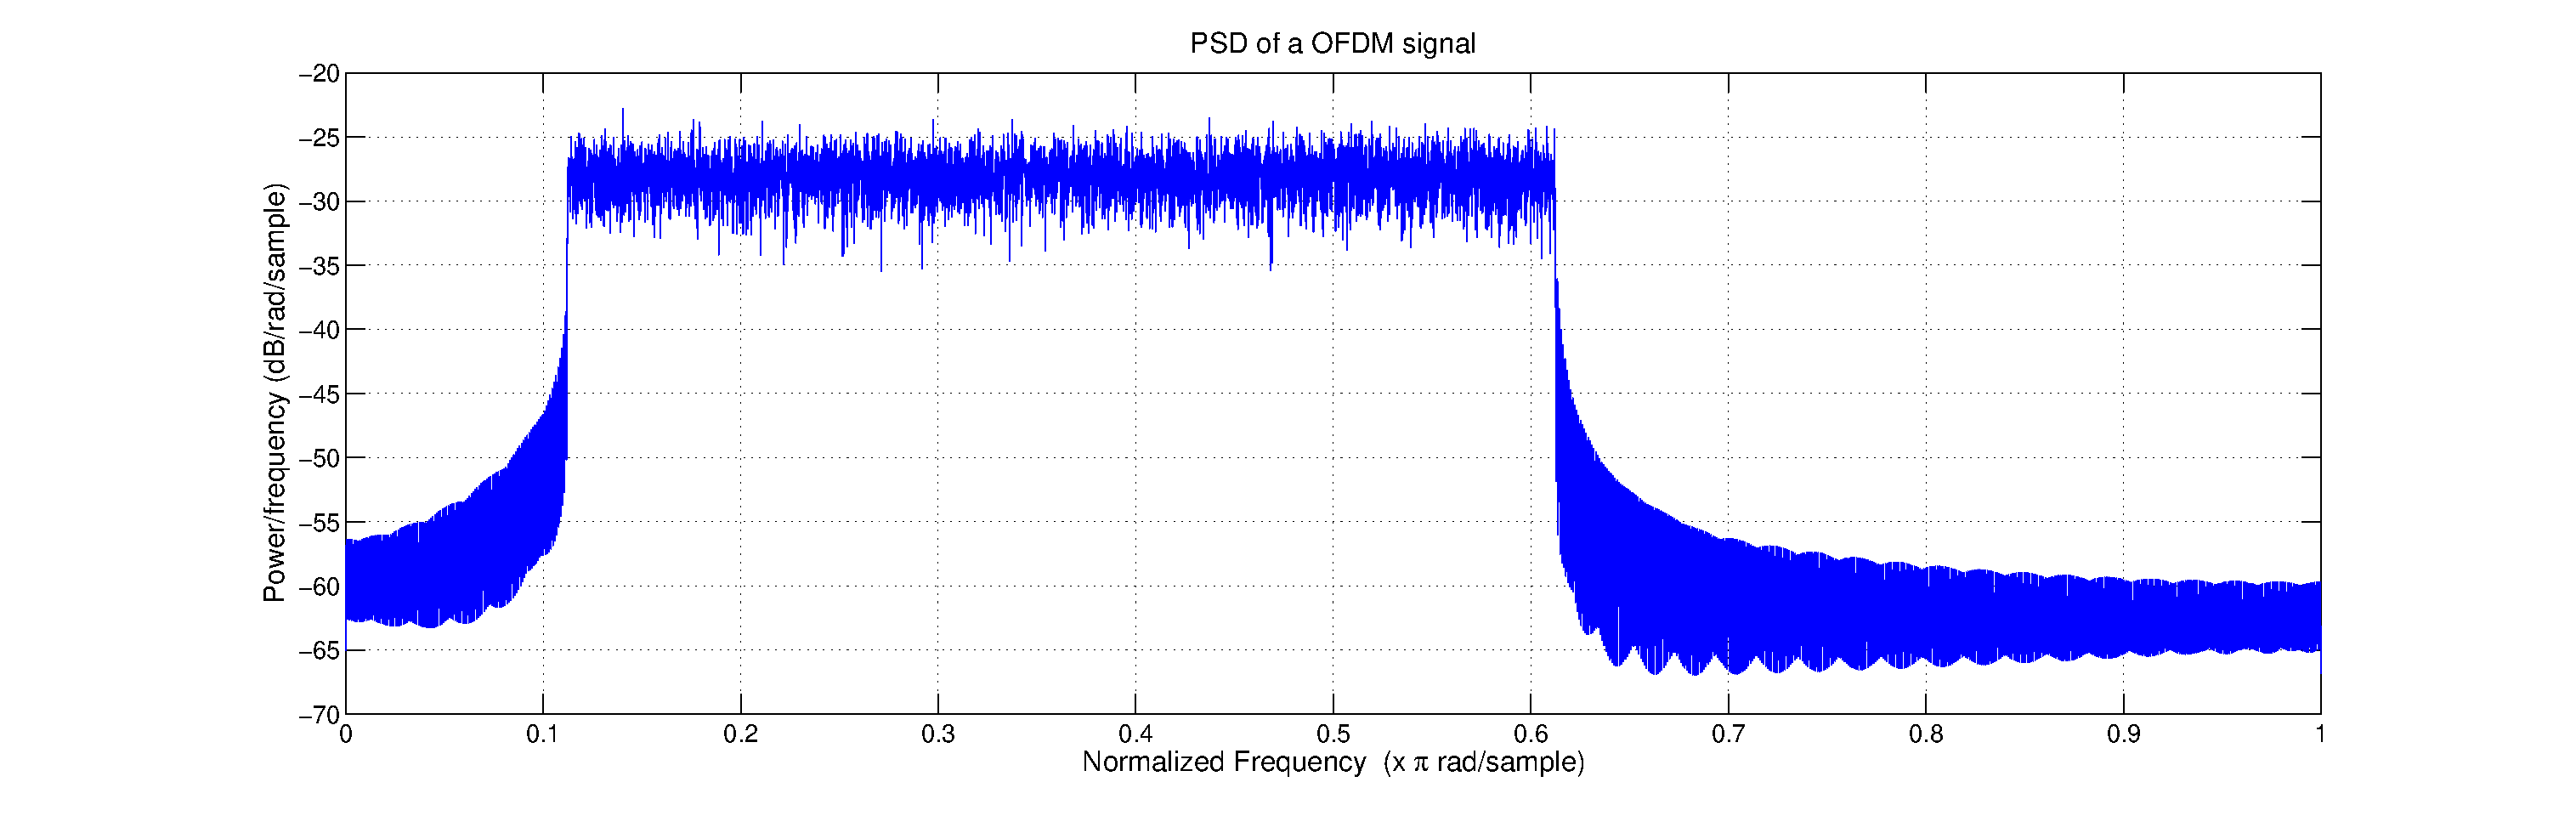
\includegraphics[width=0.9\textwidth]{psdofdm.eps}
    \subcaption{PSD of a OFDM signal}
   %% \label{}
 	\end{subfigure}
    \caption[OFDM signal in time and frequency domains.]{OFDM signal in time and frequency domains. The signal is centred at 8 kHz with a DFT size of $N=2048$, the number of active sub-carriers is $N_c =512$ using a sampling frequency of $f_s=44.1$ kHz.}
    \label{fig:ofdmsig}
\end{figure}


% %\subsubsection{OFDM impairments}
\subsubsection{OFDM Impairments}
\label{sub:OFDMimpairments}
In multi-path channels, a receiver can pick up several delayed replicas of the transmitted signal leading to ISI. To eliminate the effect of this inter symbol interference, a guard interval of $N_g$ samples is usually inserted at the beginning of each OFDM symbol. During the guard interval the transmitter can either:

\begin{itemize}
\item Zero pad (ZP) the transmission by sending a null waveform.

\item Introduce a cyclic prefix (CP), which is an exact copy of a segment of the OFDM symbol located towards the symbol end. A cyclic suffix can be used in a similar fashion.

\end{itemize}
Since ZP introduces inter-carrier interference (ICI), cyclic prefixing transmission is preferred. 
To prevent significant leakage to adjacent bands, OFDM systems usually do not transmit any data on the sub-carriers near the two edges of the allocated band. These unused sub-carriers are known as guard sub-carriers or virtual sub-carriers. The collection of all the unused sub-carriers is called the guard band. As the PSD of the OFDM signal has quite high sidelobes, to reserve a guard band contributes to minimise out-of-band emissions and thus, eases the requirements on transmitter front-end filters. Nevertheless, adoption of a guard band wastes the allocated bandwidth and decreases the spectral efficiency of the OFDM system. In addition to guard bands, some sub-carriers around DC frequency (sub-carrier index 0) should be nullified in order to evade unwanted DC and low-frequency components generated by the receiver's front-end. Other issues may arise when using of OFDM, like spectral shaping and peak-to-average power ratio. The first is discussed in section \ref{Sec:Pulse shaping}. 


An additional parameter that may influence the performance of an OFDM system is the Peak-to-Average Power Ratio (PAPR), defined as the ratio of the peak power with the average power:

\begin{equation}
PAPR = \frac{{\max {{\left| {x(t)} \right|}^2}}}{{\mathbb{E}\left\{ {{{\left| {x(t)} \right|}^2}} \right\}}}
\end{equation}

In the extreme case in which all the sub-carriers are coherent and summed up evenly, the time-domain OFDM signal will have a PAPR directly proportional to the total number of transmitted sub-carriers. In this case, the transmitter amplifier will require to handle a high dynamic range which might be impractical for some applications\footnote{The power amplifier may saturate if not biased properly, leading to intermodulation and other non-linear effects.}. Many approaches are possible in order to reduce the PAPR, such as clipping, windowing an applying clever coding techniques.     

\subsubsection{OFDM Transceiver Architecture}

A general OFDM transmitter integrates several functions including DFT processing, guard interval insertion and spectral shaping. In a receiver, besides DFT processing and guard interval removal, additional efforts are required to handle the channel-fading effect and synchronisation issues between the transmitter and receiver.
As it will be discussed in part \ref{sec:ts}, the amplitude and phase may be estimated via the use of a known training sequence. In an OFDM system, these parameters should be estimated for each of the carriers' frequencies. In the case of a time variant channel, the new estimations can be done by inserting known reference symbols (sometimes referred as pilot symbols) at regular intervals within the OFDM time-frequency grid. The effects of an amplitude varying channel and the previously mentioned grid are depicted in figure \ref{fig:ofdmchannel}.

\textcolor{red}{Add references and footnotes from books if they fit better.}
\begin{figure}[H]
 \centering
	\begin{subfigure}[H]{0.9\textwidth}
 	\centering
    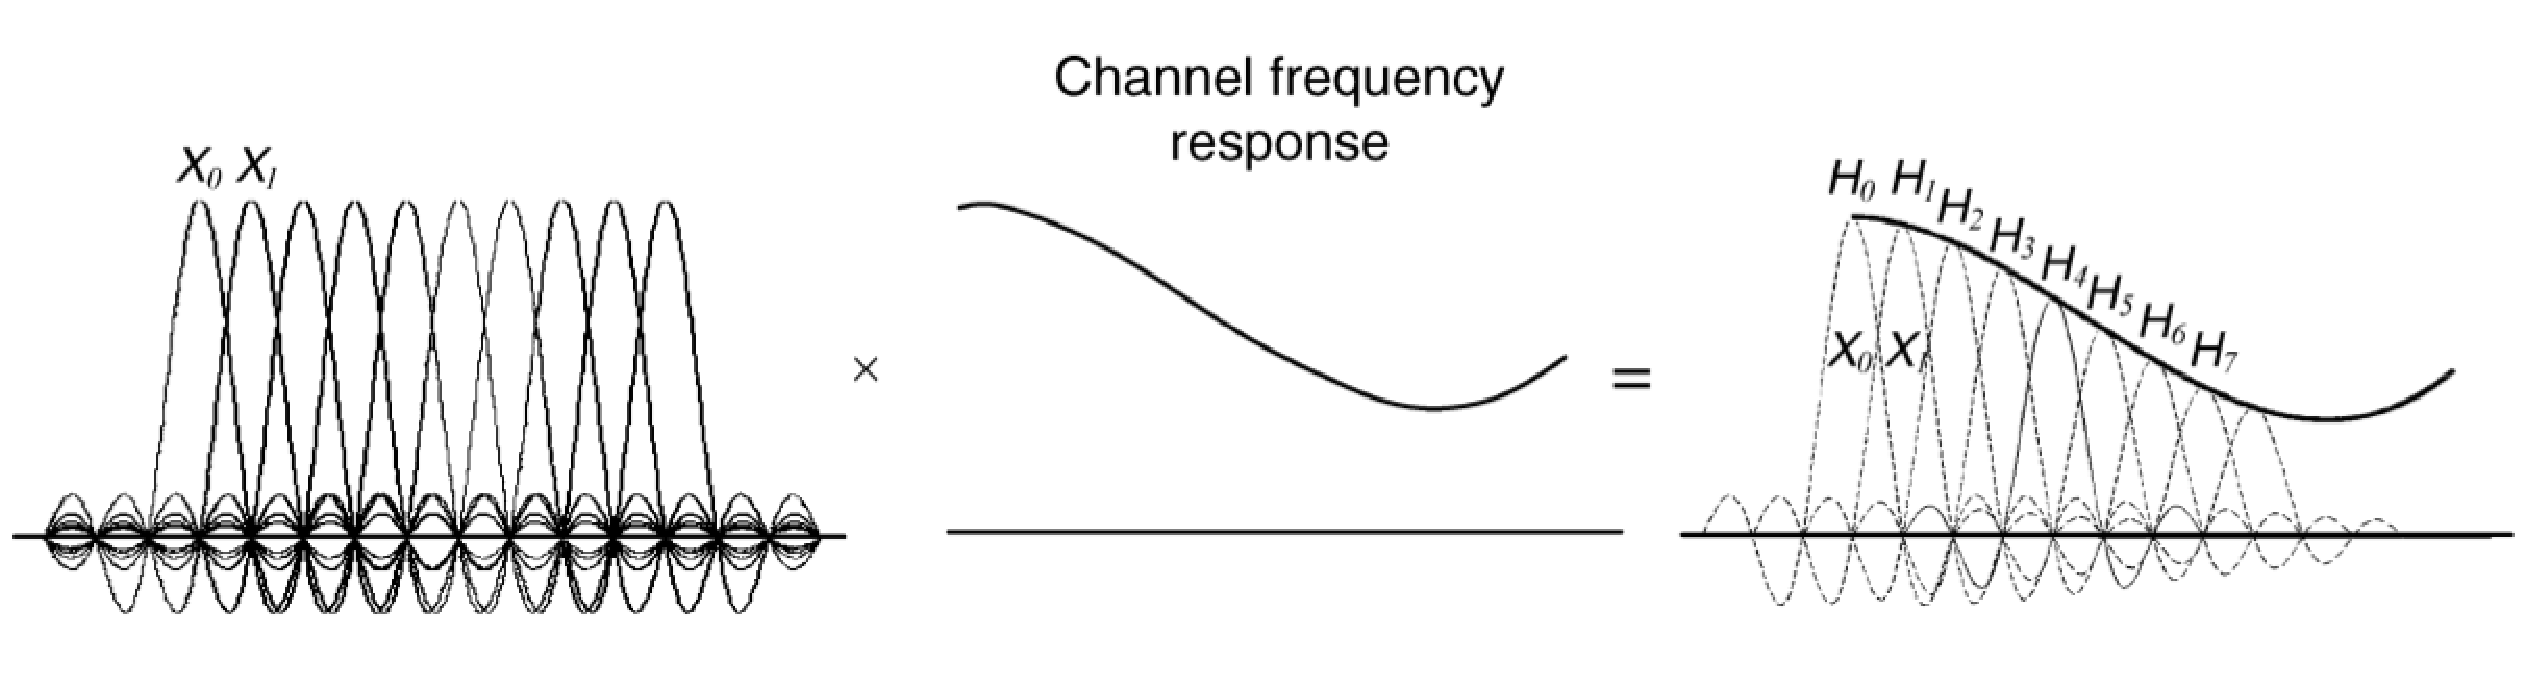
\includegraphics[width=0.9\textwidth]{ofdmchannel.pdf}
    \subcaption{Amplitude distorsion effects in each OFDM sub-carrier.}
    %%\label{}

	\end{subfigure}
	
	\begin{subfigure}[H]{0.9\textwidth}
 	\centering
    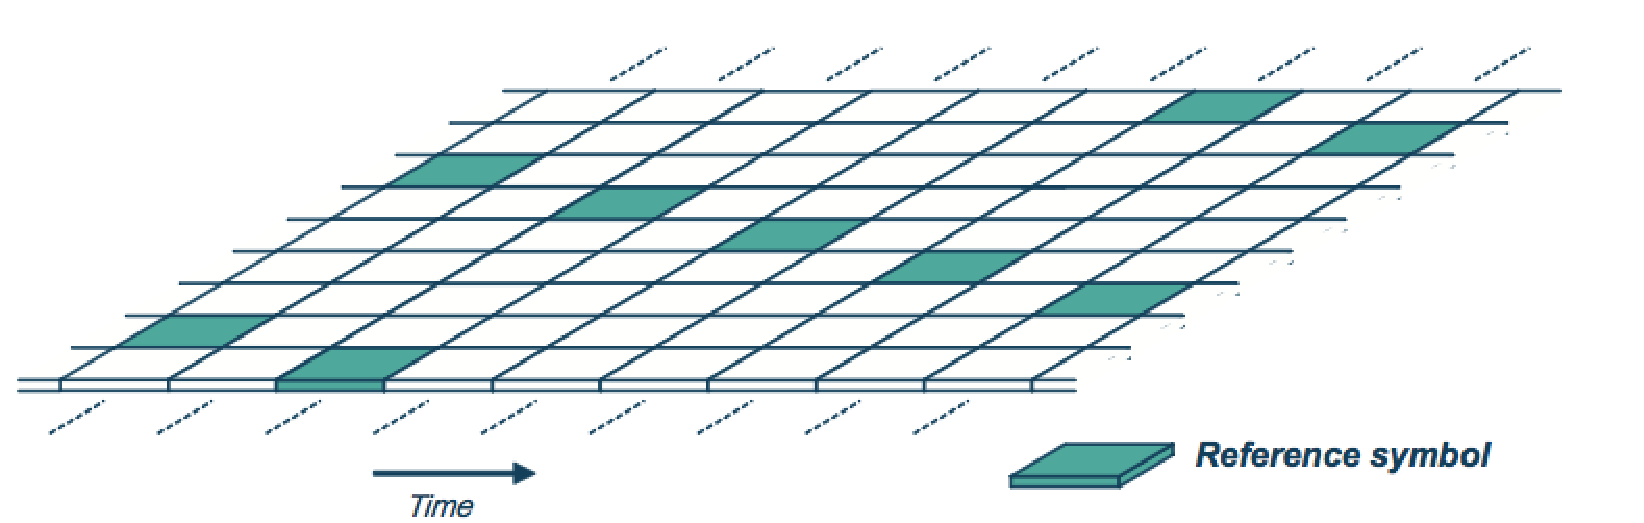
\includegraphics[width=0.7\textwidth]{ofdmgrid.pdf}
    \subcaption{Frequency-time grid containing the pilots. Reference symbols density should be chosen according to the channel properties.}
   %% \label{}
 	\end{subfigure}
    \caption[The effects of a non-flat channel and a grid containing the OFDM pilot symbols]{The effects of a non-flat channel and a grid containing the OFDM pilot symbols in time and frequency domains for channel estimation.}
    \label{fig:ofdmchannel}
\end{figure}

Therefore, in the implementation of an OFDM communication system, the following basic OFDM parameters need to be decided:

\begin{itemize}
\item Subcarrier spacing $\Delta f = \frac{1}{T_u}$. The OFDM sub-carrier spacing should be as small as possible so as to minimise the relative cyclic-prefix overhead :
 \begin{equation}
 r_{CP}=\frac{T_{CP}+T_{CS}}{T_u + T_{CP} + T_{CS}}
 \end{equation}
 However, a too small sub-carrier spacing increases the sensitivity of the OFDM transmission to Doppler spread and different kinds of frequency inaccuracies.

\item The total number of sub-carriers $N_{FFT}$. It is going to be defined by the size of the DFT.
\item The number of active sub-carriers $N_c$. This value together with $N_{FFT}$, will define the bandwidth occupied by the signal:

\begin{equation}\label{eq:OFDMbw}
W = N_c \times \Delta f = \frac{N_c}{T_u}=\frac{N_c}{N_{FFT}}\times f_s
\end{equation}

\item The length of cyclic prefix and suffix  $T_g = T_{CP} + T_{CS}$. It will determine the overall symbol time $T = T_u + T_g$. In principle, the cyclic-prefix length $T_{CP}$ should cover the maximum length of the time dispersion that is expected in the channel. 
\end{itemize}

These parameters, along with some others, determine the performance of the system and must be chosen carefully. 

Similarly at the receiving side, the inverse operations are performed after the synchronisation is completed. The process is illustrated in figure \ref{fig:ofdmtransceiver}.

\textcolor{red}{Add reference to picture}
 \begin{figure}[H]
  \centering
    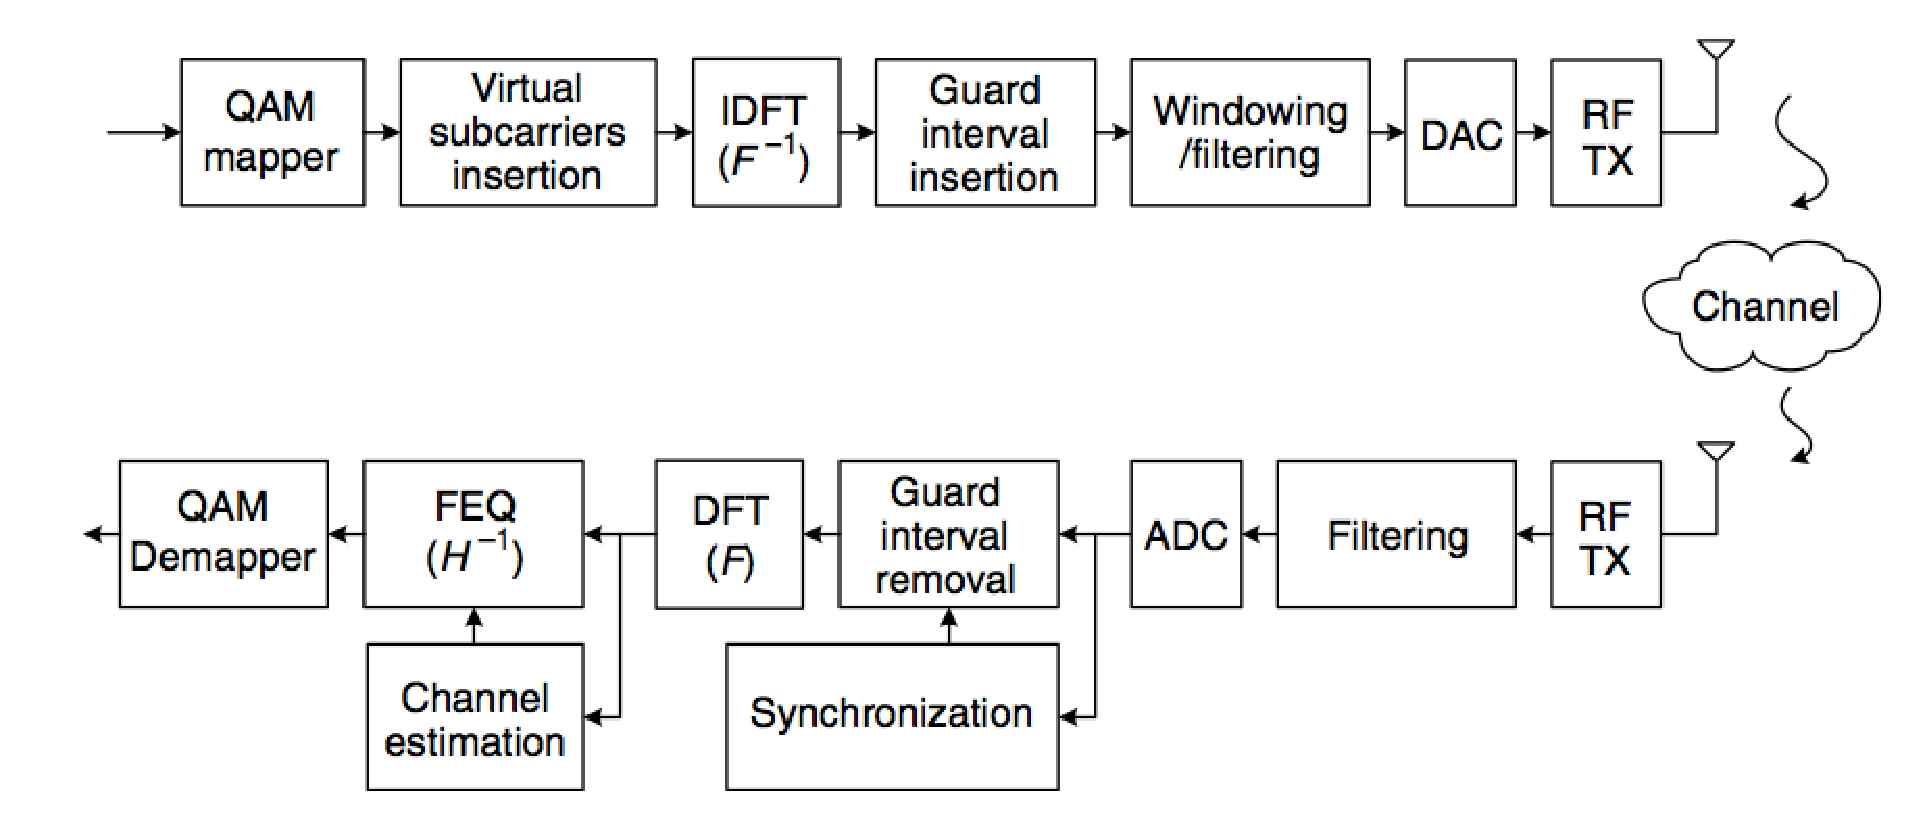
\includegraphics[width=0.8\textwidth]{ofdmtransceiver.pdf}
    \caption[OFDM transceiver using QAM symbol mapping.]{OFDM transceiver using QAM symbol mapping.}
    \label{fig:ofdmtransceiver}
\end{figure}



%
\section{Pulse Shaping}
\label{Sec:Pulse shaping}
So far we have considered the case where the modulated signal is shaped by a rectangular function inside the interval $0\leq t \leq T_s$. If the pulse shaping function $g(t)$ is a rectangular pulse of width of $T_s$, the envelope of the signal is constant. However, a rectangular pulse has very high spectral sidelobes, which means that signals must use a larger bandwidth to eliminate some of the adjacent channel sidelobe energy. Pulse-shaping is a method to reduce the sidelobe energy relative to a rectangular pulse. On the other hand, the shaping must be done in such a way that the ISI between pulses in the received signals is not introduced (or at least it is minimised). Assuming the channel model is AWGN, the effective received pulse is given by: 

\begin{equation}
p(t)=g(t) \ast c(t) \ast g^{*}(-t)=g(t) \ast g^{*}(-t) \text{, since }c(t)=\delta(t)
\end{equation}

This pulse must satisfy the Nyquist criterion, that requires the pulse to equal zero at the ideal sampling point associated with past or future symbols \cite{GoertzelPaper}: 

 \begin{equation}
 p(k{T_s}) = \left\{ \begin{array}{l}
 {p_0} = p(0),k = 0\\
 0,k \ne 0
 \end{array} \right.\ ,
 \end{equation}
 
Some examples of the pulses (also called windows) that satisfy this criterion are the rectangular, raised cosine (Hanning) and the root-raised cosine. Each pulse has advantages and disadvantages, but the last two are aimed to improve the spectral efficiency. The most common window in FSK is the Gaussian pulse, defined as: 

 
\begin{equation}\label{Eq:Gaussian Window}
g(t) = \frac{{\sqrt \pi  }}{\alpha }{e^{ - {\pi ^2}{t^2}/{\alpha ^2}}}\ ,
\end{equation}

 The parameter $\alpha$ in the gaussian window is related to the 3dB bandwidth $B_z$ of $g(t)$, and is defined as follows \cite{GoertzelPaper}:
\begin{equation}
\alpha  = \frac{{\sqrt { - \ln \sqrt {0.5} } }}{{{B_z}}}\ ,
\end{equation}
 
  Hence, the spectrum of $g(t)$ is given by: 
\begin{equation}
G(f) = {e^{ - {\alpha ^2}{f^2}}}\ ,
\end{equation}

The different window characteristics are illustrated in figure \ref{fig:wc}, and the effects when they are applied to a simple BFSK system are depicted in figure \ref{fig:wcomp}.
 \begin{figure}[H]
 \centering
  \label{fig:wincar}
\begin{subfigure}[H]{1\textwidth}
 \centering
    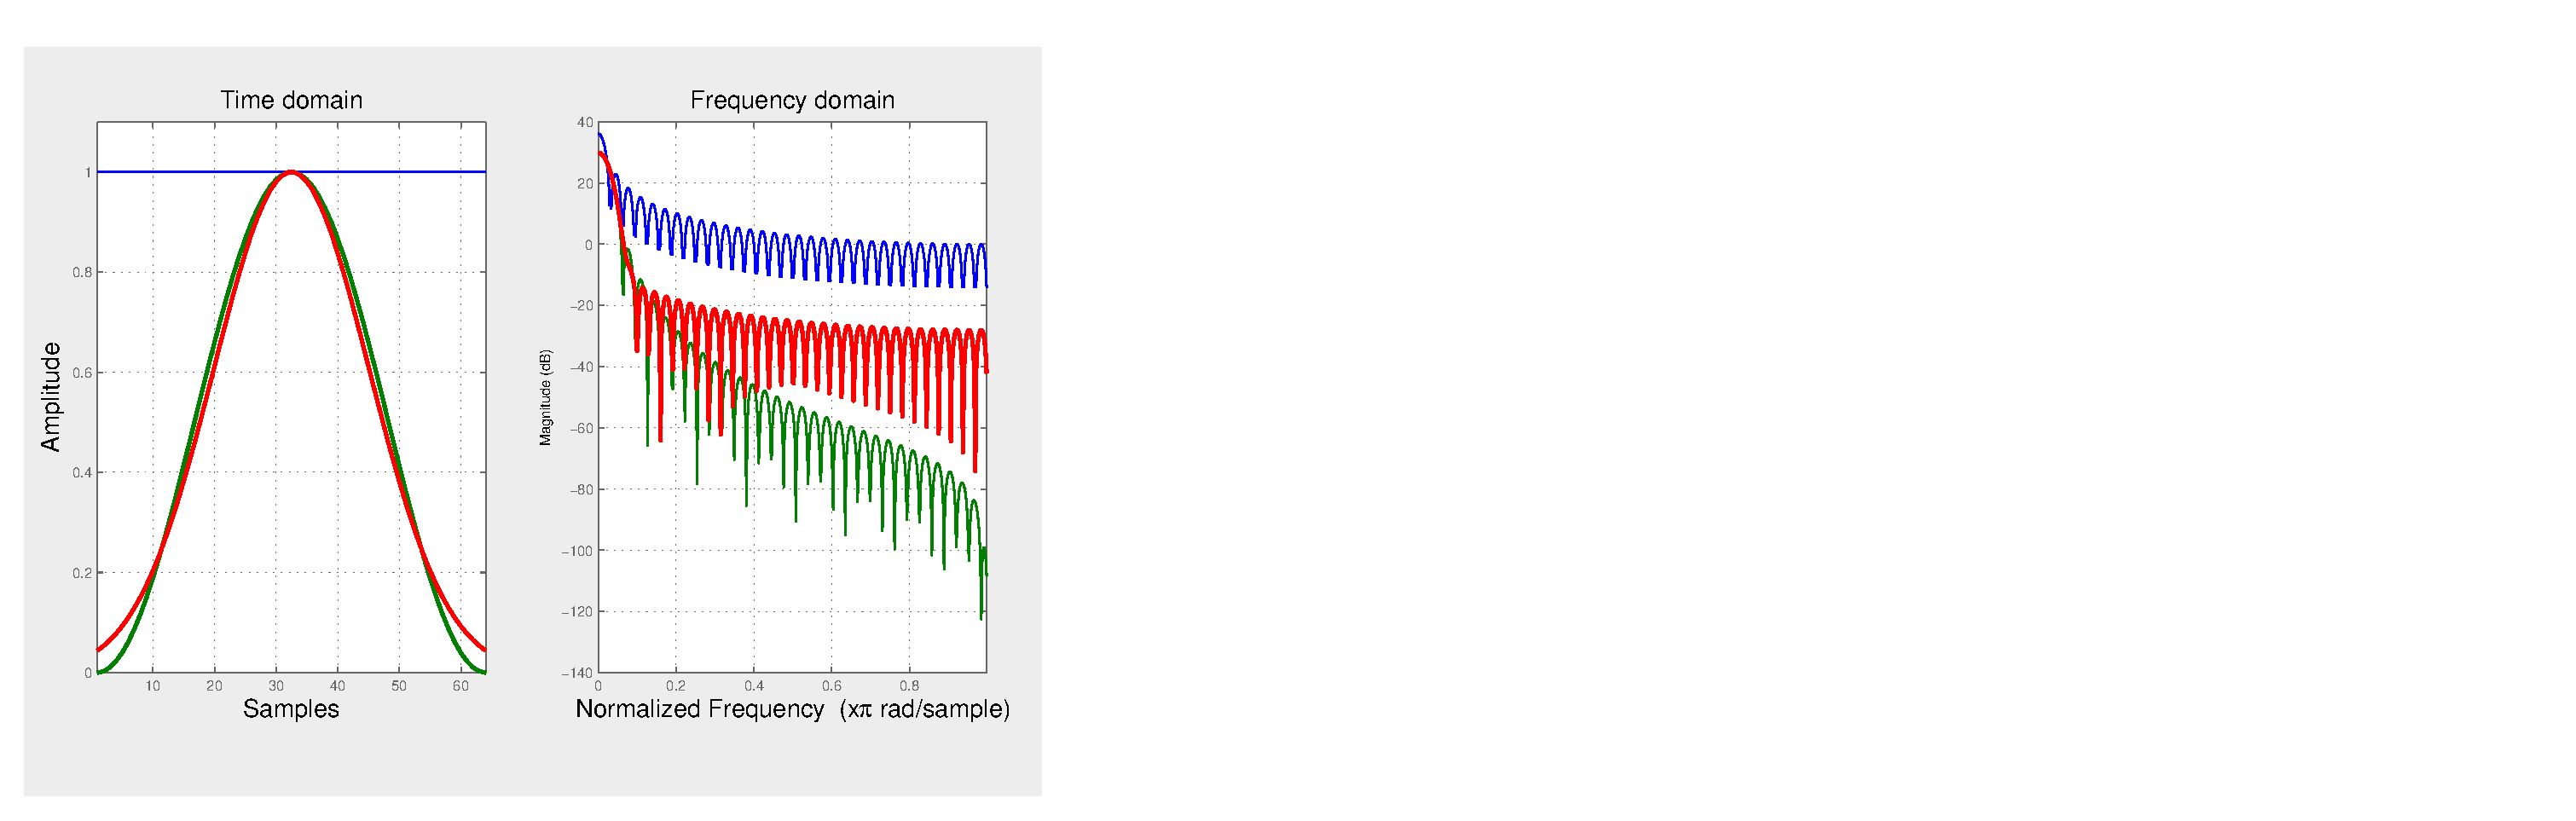
\includegraphics[scale=0.45, trim=0 0 30cm 0, clip=true]{wincomp.eps}
    \subcaption{Different windows in time and frequency domain. Blue, red and green lines correspond to the rectangular, Gaussian and Hanning window, respectively.}
    \label{fig:wc}
\end{subfigure}

\qquad
\qquad

\begin{subfigure}[H]{1\textwidth}
 \centering
    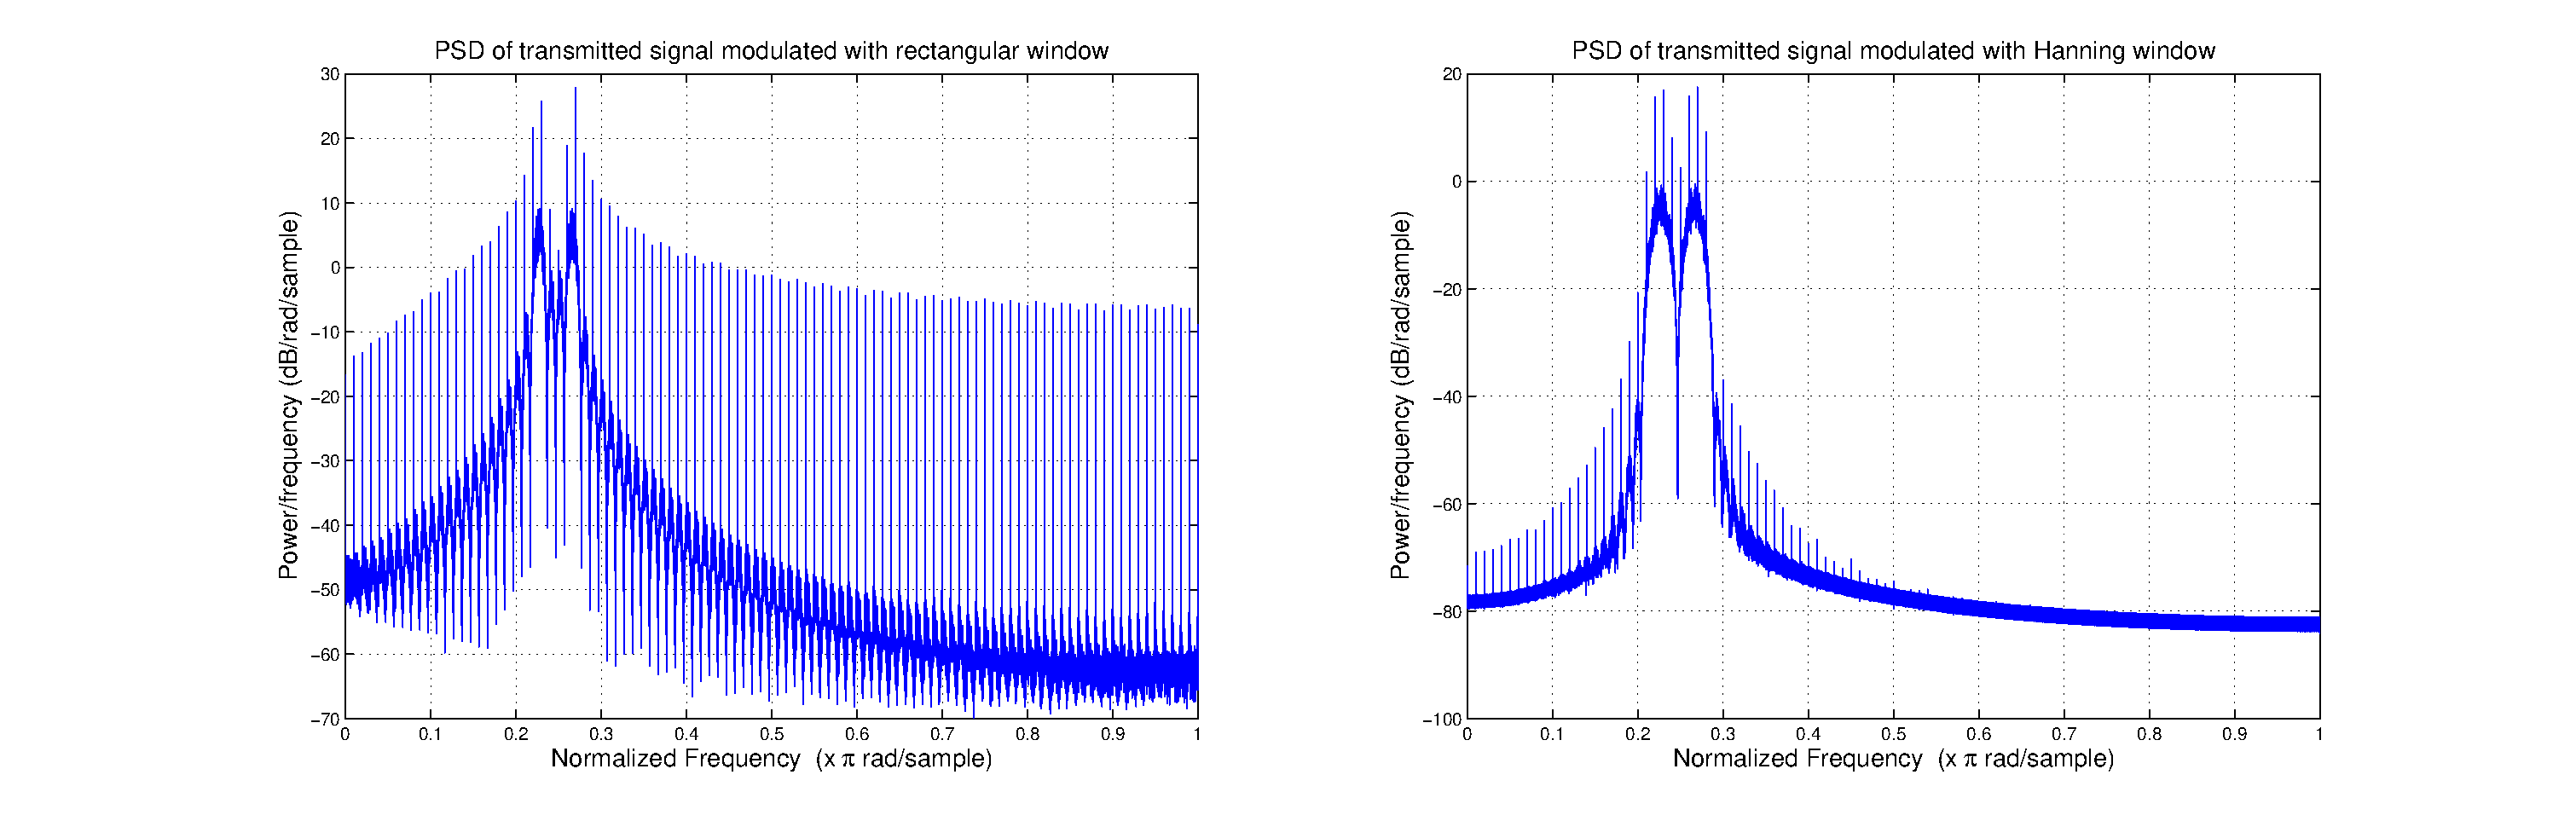
\includegraphics[scale=0.38]{txwinrectVShann.eps}
    \subcaption{PSD of a transmitted BFSK signal using rectangular and Hanning windows for pulse shaping.}
    \label{fig:wcomp}
    
    \end{subfigure}
    
    \caption[Effects of pulse shaping in a modulated signal]{Effects of pulse shaping in a modulated signal. Some windows smooth the sidelobes of the transmitting the signal, reducing the bandwidth consumption.}
    \label{fig:main}
\end{figure}

We see that if we make $\alpha$ large, it will result in a higher spectral efficiency. The Gaussian pulse does not satisfy the Nyquist criterion and therefore the pulse shape introduces ISI, which increases as $\alpha$ gets larger. Therefore, improving spectral efficiency by increasing $\alpha$ leads to a higher ISI level creating an irreducible error floor from this self-interference. Thus, the variable $\alpha$ should be chosen with care. The Gaussian window effect can be seen in figure \ref{fig:gaussianalpha}.

 \begin{figure}[H]
  \centering
    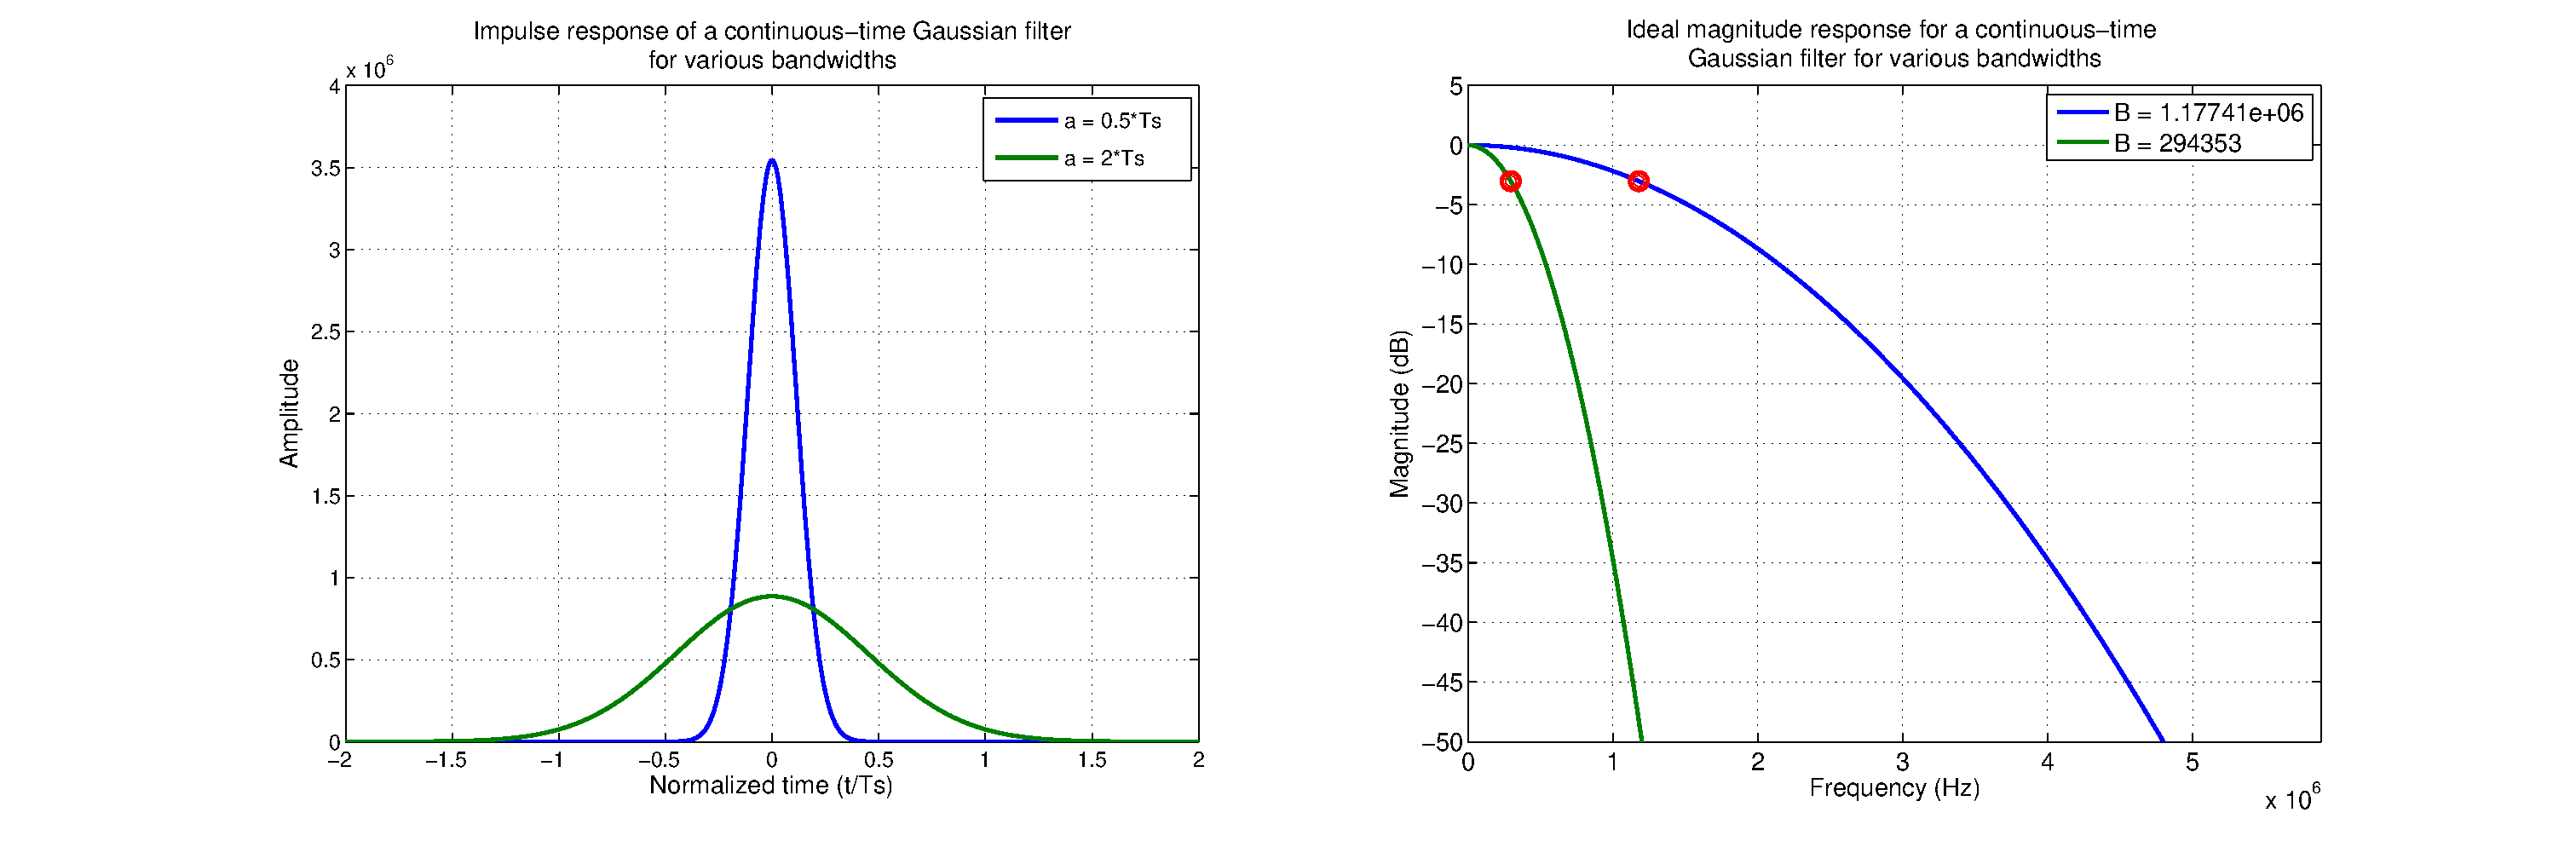
\includegraphics[width=1\textwidth]{gausswinalpha.eps}
    \caption[Ideal Gaussian filter with different values of $\alpha$]{Ideal Gaussian filter with different values of $\alpha$. The tradeoff between high spectral efficiency and ISI reduction is clear. A large $\alpha$ increases the efficiency but the amplitude for $t/T_s > 1$ is not zero, leading to ISI.}
    \label{fig:gaussianalpha}
\end{figure}  

Likewise, there are other windows that provoke similar effects when applied to shape the pulses of a digital signal. In general, such windows have a disparate effect in the adjacent bands suppression. For instance, the root-raised cosine pulse shape reduces the sidelobes more significantly by selecting the right roll-off parameter (also denoted as $\alpha$ ). But in this case, the effect of ISI is more significant than for the case of the Gaussian pulse and therefore, better ways to handle the ISI must be used in the system. 


\section{Synchronisation}
\label{sec:ts}

Carrier synchronisation is an extremely important parameter for the performance of the system. Up to this point we have assumed that the receiver is perfectly synchronised with the transmitter and the only channel impairment is AWGN. However in practice, it is often found that there is also uncertainty because of the randomness of some signal parameters caused by distortion in the transmission medium and due to hardware constraints. One of the most common random parameters is the carrier phase, especially for narrowband signals. A timing error in sampling may lead to a series of ISI components that converge and affect the overall system performance. 

There are two basic modes of synchronisation in the reception of a digitally modulated signal:
\begin{enumerate}
\item \textbf{Carrier Synchronisation.}  When coherent detection is used, knowledge of both  frequency and phase of the carrier are necessary. The process of estimating such parameters is called carrier recovery.

\item \textbf{Clock recovery.} To perform demodulation the receiver has to know the instants of time that at which the modulation in the transmitter changes its state. In other words, the receiver has to know the starting and finishing point of the individual symbols so that it may determine when to sample. The estimation of these times is called symbol synchronisation. 
\end{enumerate}

The synchronisation algorithm is crucial for the operation of the system. Its task is to find the best sampling time for the sampling device. Ideally, the MF should be sampled such that the SNR for the decision variable is maximised. For a rectangular pulse shape the best sampling time $t_{samp}$ is at the peaks coming out from the matched filter (see figure \ref{fig:mfpeaks}).

 \begin{figure}[H]
  \centering
    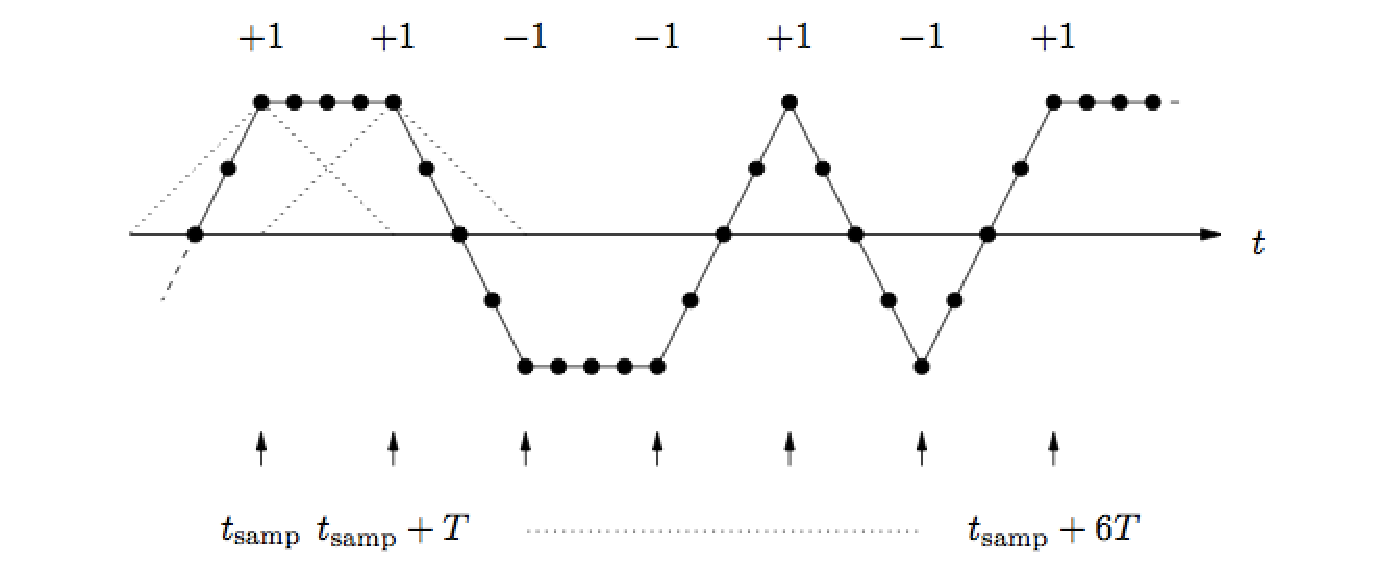
\includegraphics[width=0.7\textwidth]{mfpeaks.pdf}
    \caption[Matched filter output for successive signalling in absence of noise]{Matched filter output for successive signalling in absence of noise. The small arrows illustrate the preferred sampling instants \cite{ProjectEQ2310}.}
    \label{fig:mfpeaks}
\end{figure}

One of the most common synchronisation techniques is to use a training sequence. When the signal is received, the receiver is able to identify the training sequence and recover the symbol time by cross-correlating the samples after the matched filter with a locally generated time-shifted replica of the training sequence. This algorithm can be either applied directly to the received samples, by correlating them with a modulated training sequence (resolution of one sample, but very sensitive), or applied at the symbol level (resolution of $T/Q$, where $Q$ is the number of samples per symbol). We consider the last option to simplify. If ${\left\{ {c(n)} \right\}_{n = 0}^{L - 1}}$ is the locally generated symbol-spaced replica of the training sequence of length $L$, [$t_{start},t_{end}$] represents the search window and $r(n)$ denotes the output from the matched filter. The sampling instant can be found as \cite{ProjectEQ2310}:

\begin{equation}
{t_{samp}} = \arg \mathop {\max }\limits_{{t_{samp}} \in [{t_{start}},{t_{end}}]} \left| {\sum\limits_{k = 0}^{L - 1} {r(kQ + {t_{samp}})^*c(k)} } \right|
\end{equation}

The correlation properties of the training sequence are important as they affect the estimation accuracy. Ideally, the autocorrelation function for the training sequence should be equal to a delta pulse, which means it should have a zero correlation everywhere except at lag zero. Therefore, the training sequence should be carefully designed. For example, better results for the correlation are obtained if the training sequence is modulated with a different frequency or pulse shape than the rest of the signal. Such effects are depicted in figure \ref{fig:tscomp}. 

\begin{figure}[H] 
  \begin{subfigure}[b]{0.5\linewidth}
    \centering
    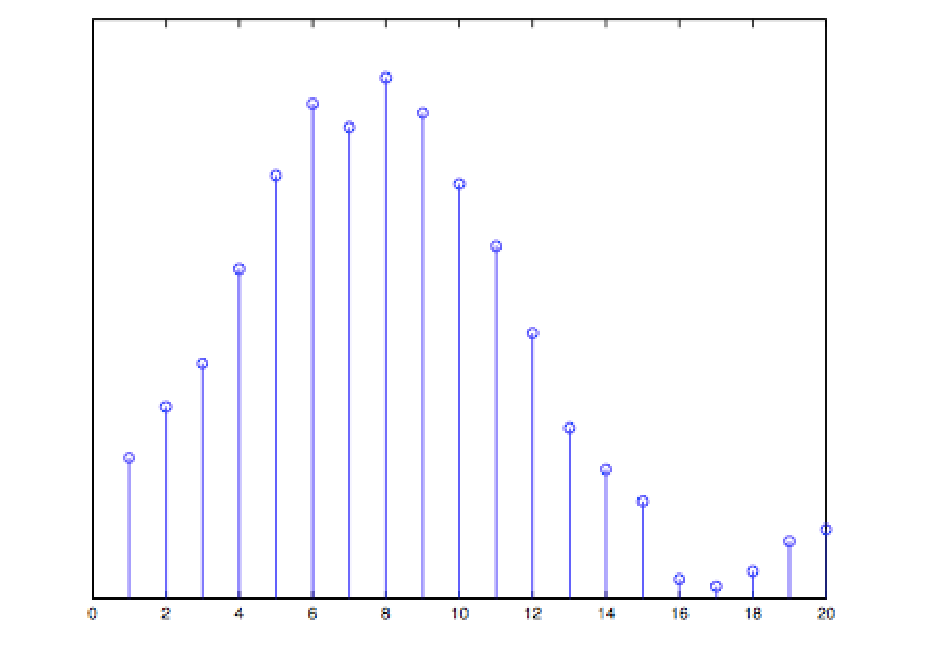
\includegraphics[width=1\linewidth]{ss.pdf} 
    \caption{Symbol spaced cross-correlation. In this example, the delay is estimated to be 8 and therefore the system should be sampled at $8+kQ$, with $k=0 , 1, 2,\cdots N$.} 
    \label{fig:a} 
    \vspace{4ex}
  \end{subfigure}%% 
  \quad
  \begin{subfigure}[b]{0.5\linewidth}
    \centering
    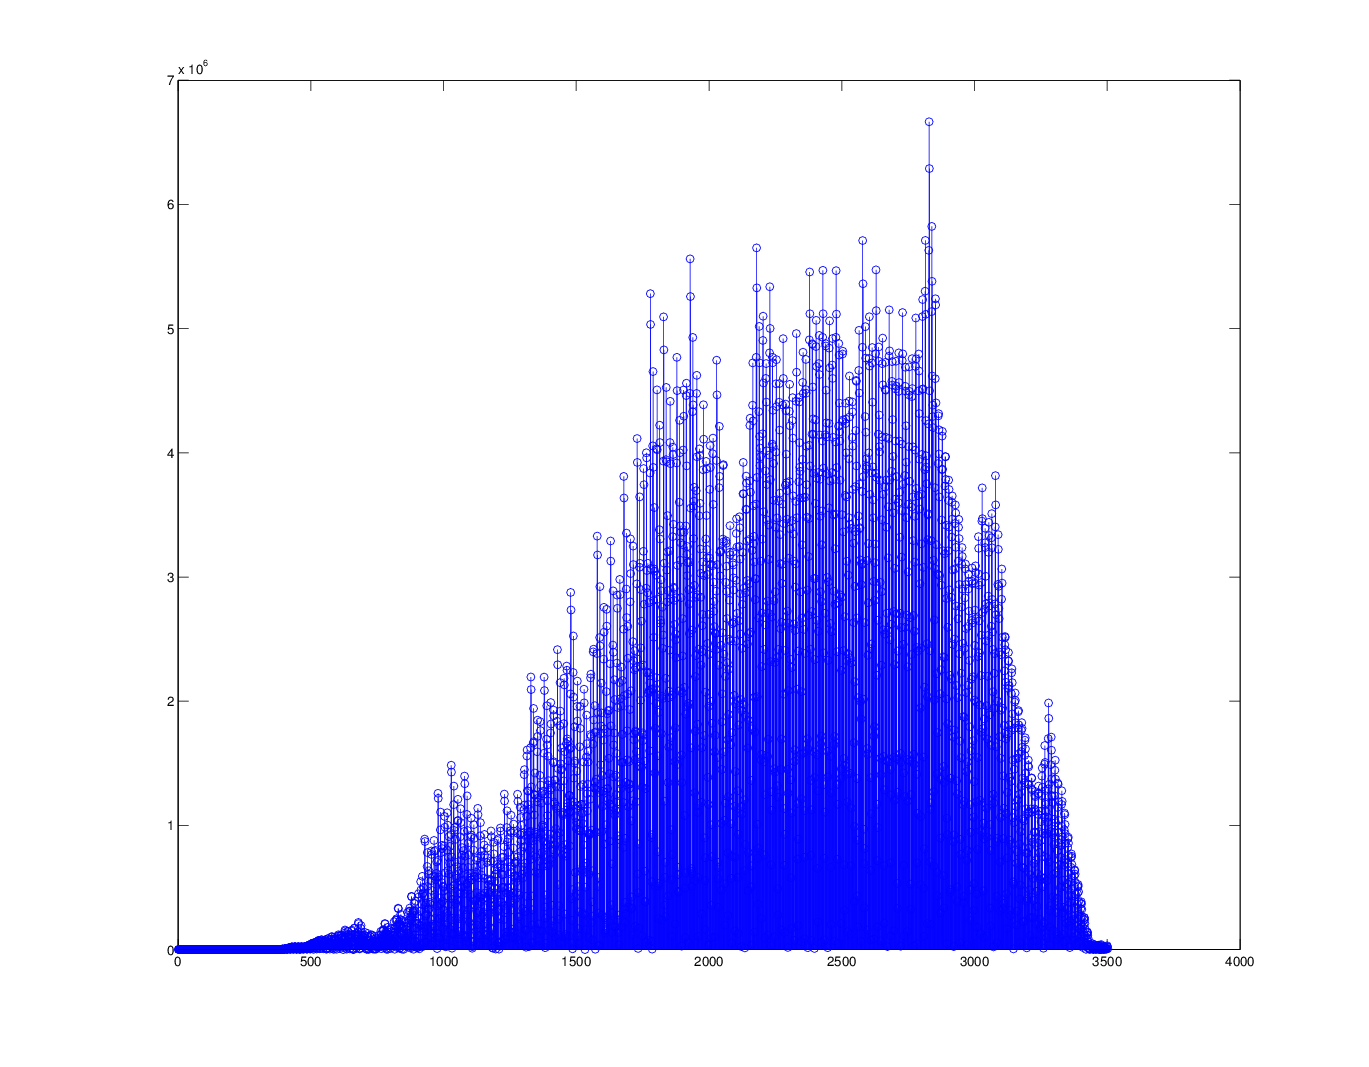
\includegraphics[width=1\linewidth]{20.png} 
    \caption{One sample resolution cross-correlation with training sequence of length 20 symbols.  \\} 
    \label{fig7:b} 
    \vspace{4ex}
  \end{subfigure} 
  \quad
  \begin{subfigure}[b]{0.5\linewidth}
    \centering
    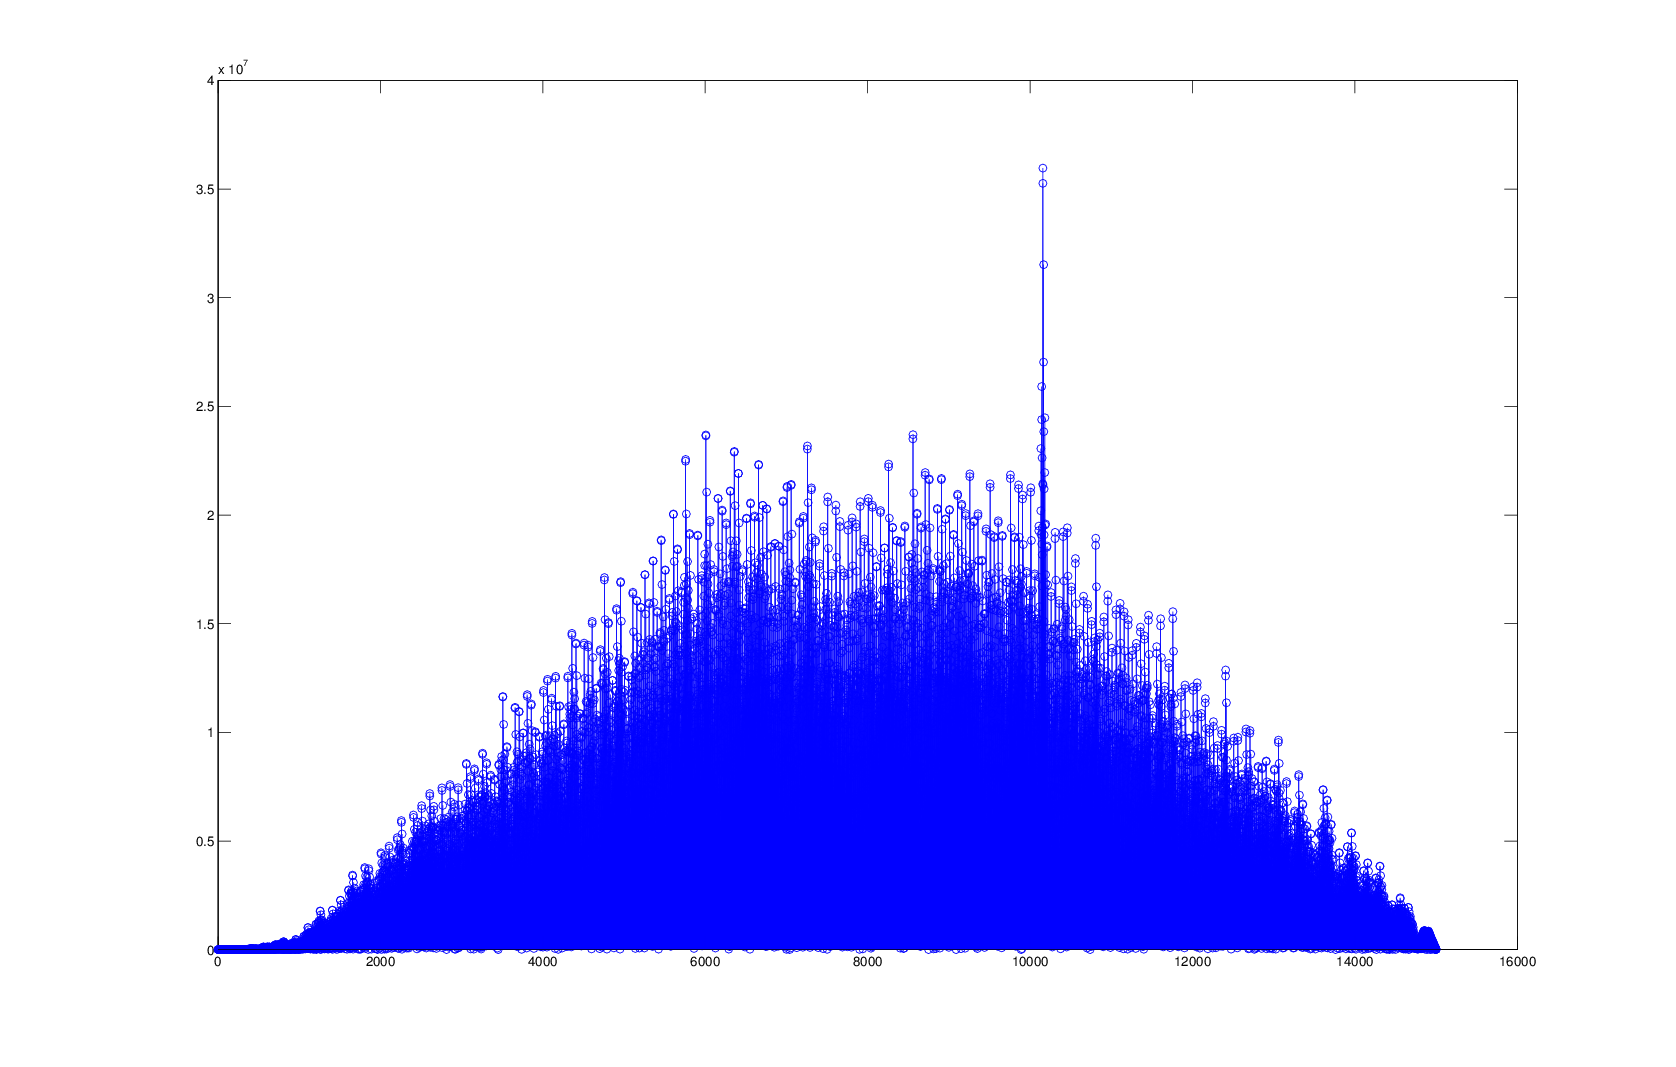
\includegraphics[width=1\linewidth]{100eq.png} 
    \caption{One sample resolution cross-correlation with training sequence of length 100 symbols and equal frequency to rest of transmission.} 
    \label{fig7:c} 
  \end{subfigure}%%
  \quad
  \begin{subfigure}[b]{0.5\linewidth}
    \centering
    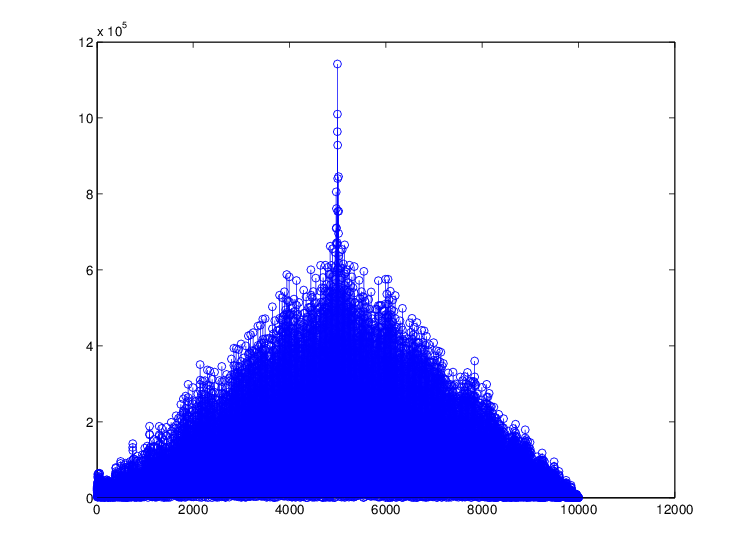
\includegraphics[width=1\linewidth]{100dif.png} 
    \caption{One sample resolution cross-correlation with training sequence of length 100 symbols and different frequency to rest of transmission.} 
    \label{fig7:d} 
  \end{subfigure} 
  \caption[Training sequence algorithm/length/modulation comparison]{Training sequence algorithm/length/modulation comparison.}
  \label{fig:tscomp} 
\end{figure}

\subsection{Synchronisation in MQAM Systems}
\label{subsec:MQAMsynch}
The basic operations required by an all digital MQAM receiver are illustrated in figure \ref{fig:rxMQAM}. The quadrature down-conversion and matched filter operations produce estimates of the quadrature amplitudes that are the basis of the data decisions. The role of carrier phase synchronisation is to perform the quadrature down-conversion using phase coherent replicas of the quadrature carriers.

 \begin{figure}[H]
  \centering
    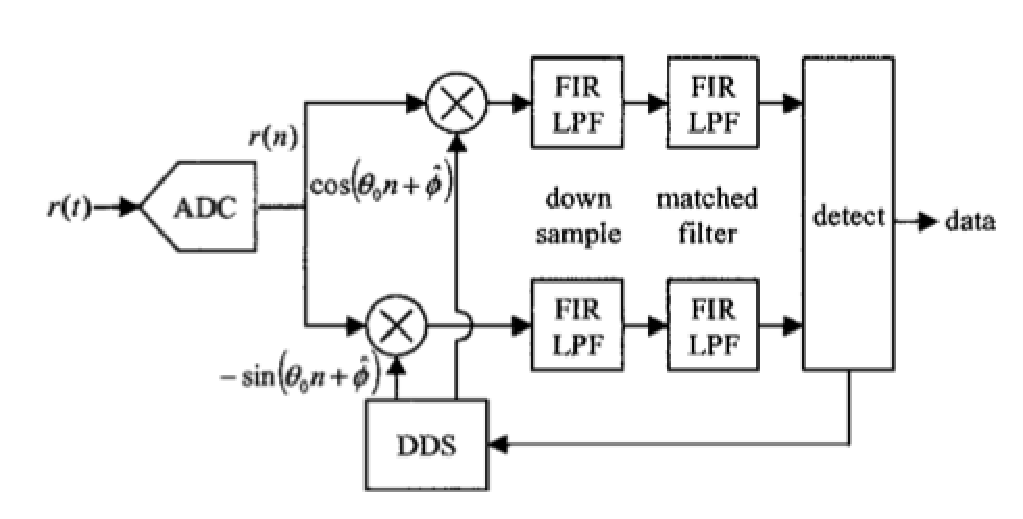
\includegraphics[width=0.6\textwidth]{rxMQAM.pdf}
    \caption[Block diagram of basic QPSK/QAM digital receiver]{Block diagram of basic QPSK/QAM digital receiver. In the digital implementation, the VCO takes the form of a direct digital synthesiser (DDS).}
    \label{fig:rxMQAM}
\end{figure}

There are many options for implementing carrier phase and frequency synchronisation in a digital communication system. At the heart of all synchronisers there is the Phase-Locked Loop (PLL). An all-digital receiver can be implemented with a digital phase-locked loop (DPLL), as shown in figure \ref{fig:DPLL}. The phase detector is implemented using the arctangent suggested by the \emph{ATAN} block. The complexity of the phase detector can be reduced by computing a signal proportional to the sine of the phase difference. The phase error is computed comparing the phase difference between the received signal $x(n) + jy(n)$ and the closest constellation point $\hat{I}(n) + j\hat{Q(n)}$, as illustrated in figure \ref{fig:PD1}.

 \begin{figure}[H]
 \centering
\begin{subfigure}{0.5\textwidth}
 \centering
    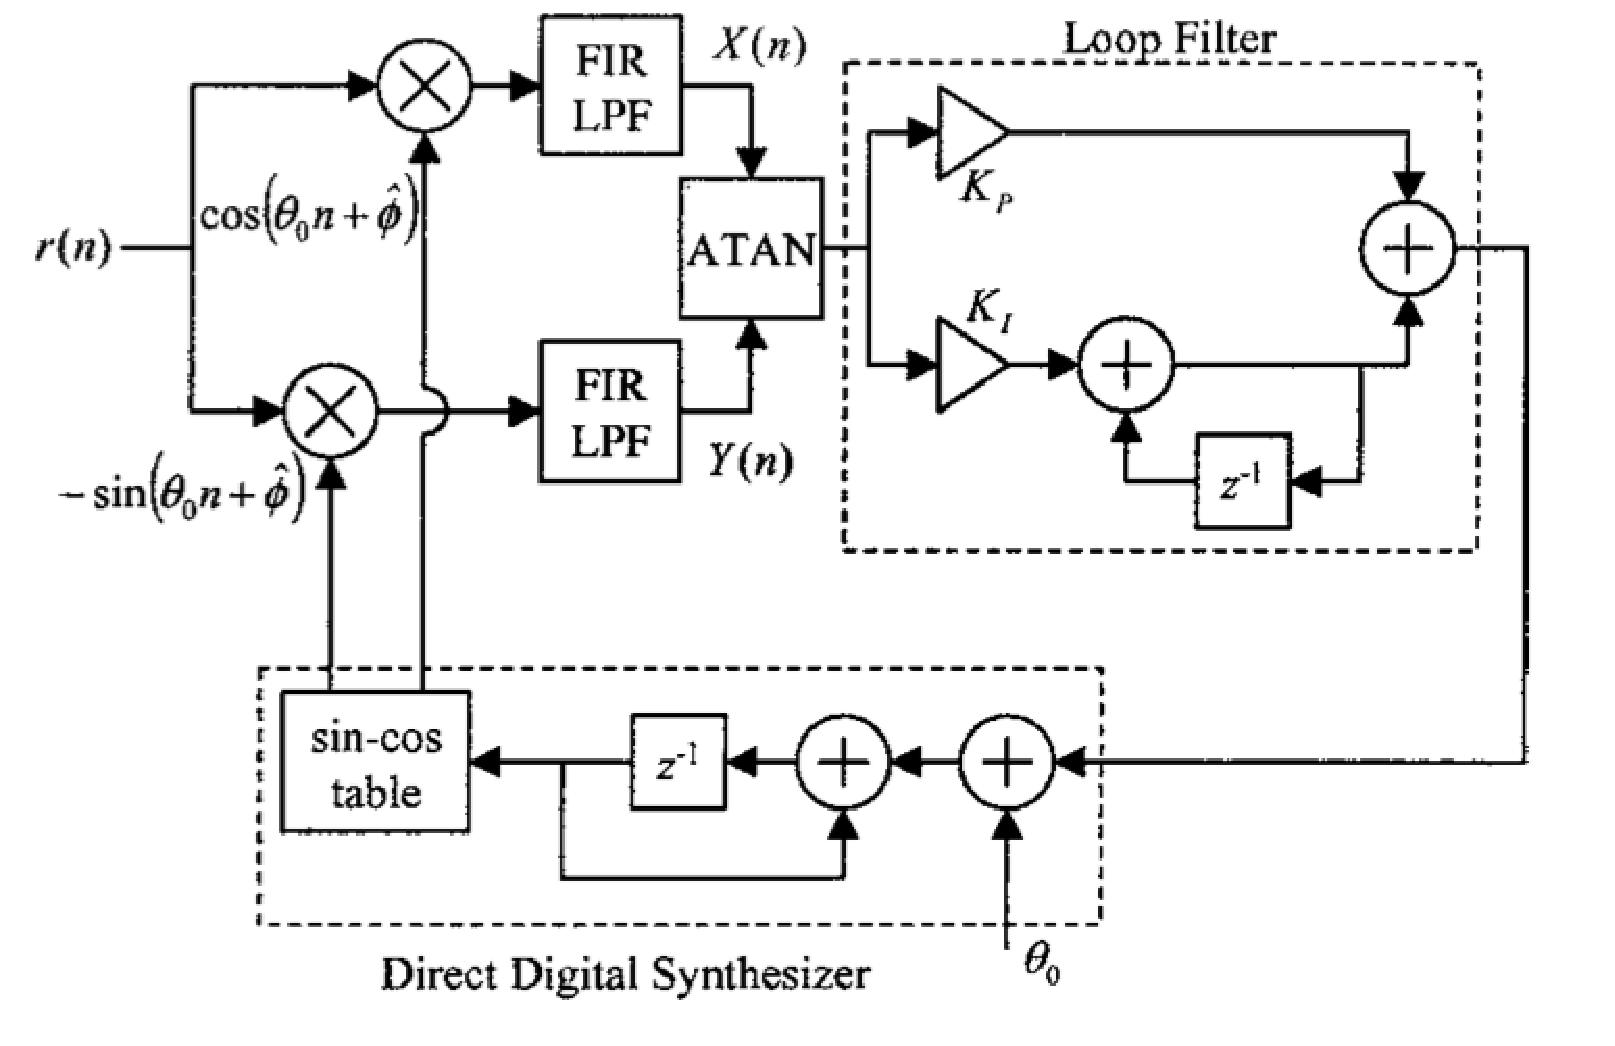
\includegraphics[width=0.9\linewidth]{DPLL.pdf}
    \caption{Digital phase locked loop for carrier phase \\ synchronisation. \\}
    \label{fig:DPLL}
\end{subfigure}%
\begin{subfigure}{0.5\textwidth}
 \centering
    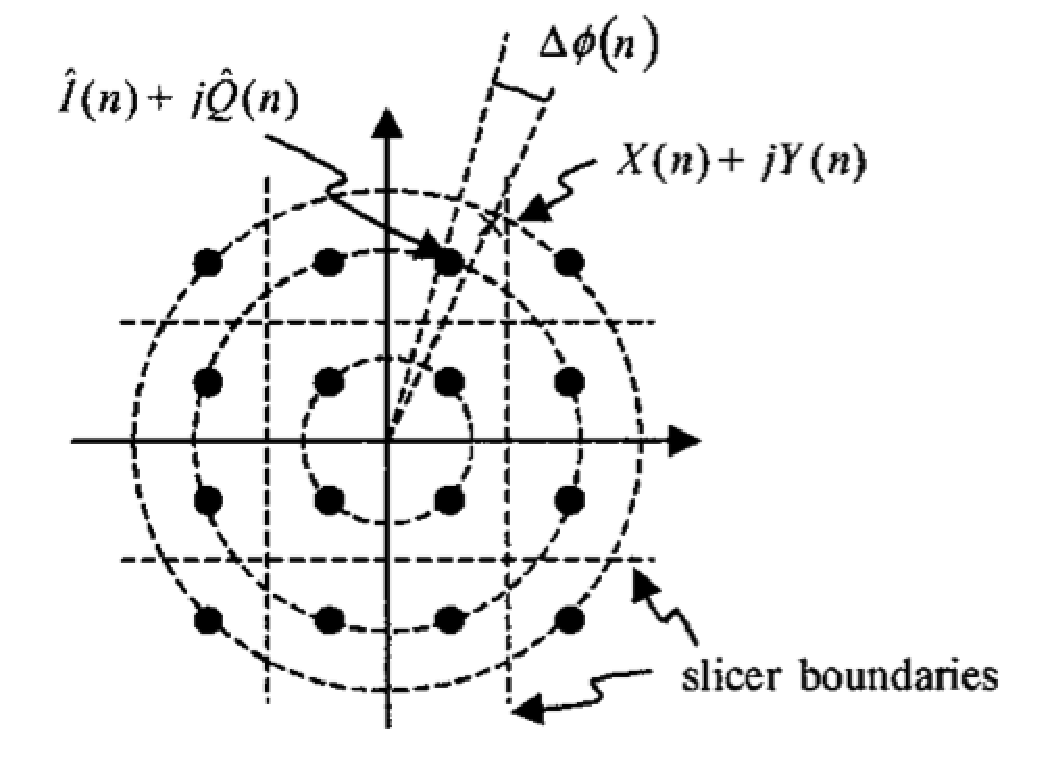
\includegraphics[width=0.7\linewidth]{PD.pdf}
    \caption{16-QAM constellation with decision boundaries and phase error.}
    \label{fig:PD1}
    \end{subfigure}
    \caption[Carrier phase estimation diagrams]{Carrier phase estimation diagrams \cite{CarrierSynchPaper}.}
    \label{fig:carrierphase}
\end{figure}

The initial phase estimation can be done using the procedure described above, taking into account the training sequence is known at transmitter and receiver. Let's assume the channel causes a rotation of $\varphi$ to the symbol constellation. The value of $\varphi$ can be computed using the element-wise multiplication of the received symbol with the complex conjugate of a modulated training sequence replica and then averaging over the sequence. In other words, if ${\left\{ {\tilde r(n)} \right\}_{n = 0}^{L - 1}}$ denotes the $L$ received symbols, and ${\left\{ {c(n)} \right\}_{n = 0}^{L - 1}}$ the local replica of the complex training sequence, the estimate of the phase offset can be obtained as \cite{ProjectEQ2310}:

\begin{equation}
\hat \varphi  = \frac{1}{L}\sum\limits_{k=0}^{L - 1} {\arg (\tilde r(k)c(k)^*)}
\end{equation}

The longer the training sequence, the better the phase estimate as the influence from the noise decreases. On the other hand, a long training sequence reduces the amount of payload that can be transmitted during a given time.

\subsection{Phase Rotation}
\label{subsec:Phase rotation}
Another problem that may be faced in a real implementation is the Doppler shift introduced during the transmission, which causes an additional rotation to the constellation (relative the initial rotation). This frequency offset could be the result of relative motion between the transmitter and receiver. That would be the case of a mobile terminal travelling away or towards a receiver. It could also be attributed to small frequency variations of the various synthesisers in both the transmitter and receiver, that normally depend on time and temperature. In order to overcome this problem, at least two approaches are possible. The first is to introduce a training sequence in the data so that, a new phase estimation can be computed. This results in a lower rate. The second solution is to divide the decisions into various small blocks (of a predefined size) in which the offset does not influence the decision. Then, we estimate the phase rotation from the nearest points and rotate the constellation for future decisions. In this way the rate is not affected but, a correct decision in each block is assumed. The frequency offset effect is shown in  figure \ref{fig:phaseoff}, where a 16-QAM signal of 5 seconds is transmitted. 


 \begin{figure}[H]
 \centering
\begin{subfigure}{0.32\textwidth}
 \centering
    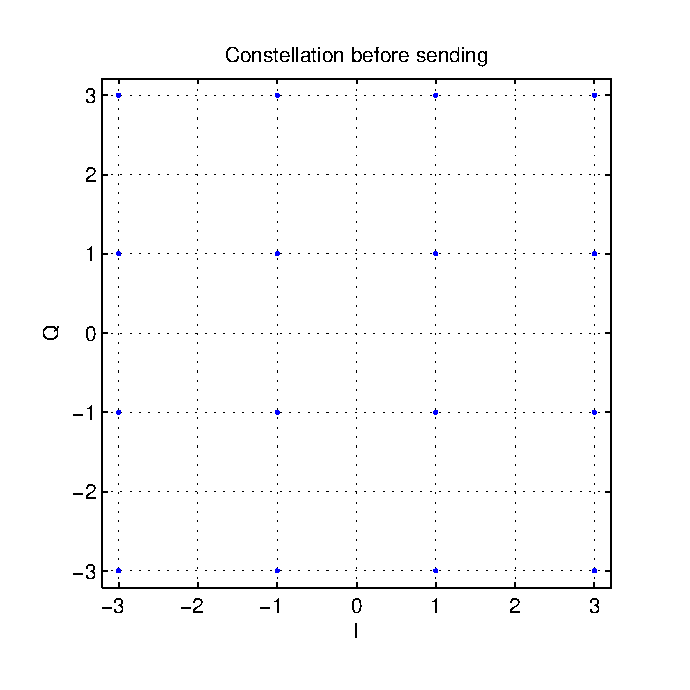
\includegraphics[width=0.8\linewidth]{tx_const.eps}
    \caption{Transmitted constellation.}
    \label{fig:DPLL2}
\end{subfigure}%
\begin{subfigure}{0.32\textwidth}
 \centering
    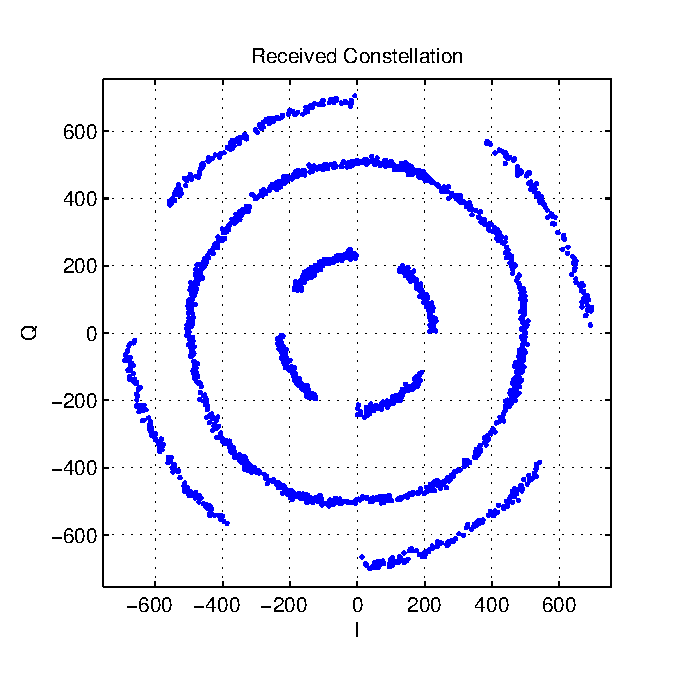
\includegraphics[width=0.8\linewidth]{rx_const.eps}
    \caption{Received constellation.}
    \label{fig:PD2}
    \end{subfigure}
    \begin{subfigure}{0.32\textwidth}
 \centering
    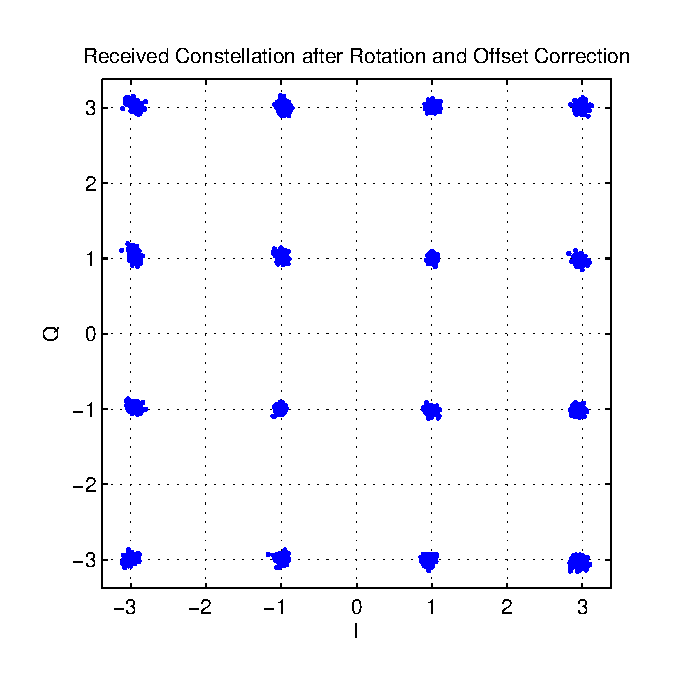
\includegraphics[width=0.9\linewidth]{rx_const_after.eps}
    \caption{Received constellation after phase correction.}
    \label{fig:PD3}
    \end{subfigure}
    \caption[Example of frequency offset in a 16-QAM constellation]{Example of frequency offset in a 16-QAM constellation with decision boundaries.  }
    \label{fig:phaseoff}
\end{figure}

%By trying different time-shifts in steps of $\frac{T}{Q}$, where $Q$ is the number of samples per symbol, the symbol timing can be found with a resolution of  $\frac{T}{Q}$.



\section{Channel Equalisation}
\label{sec:chanEQ}
The performance of a digital system is constrained by the type of channel in which the implementation is done. In our case theoretically, we have a nearly-ideal low-pass channel with low noise variance and limited up to about 20 kHz. However, the phone's audio card introduces a non-linear distortion that affects the signal output and causes attenuation around 6kHz (see figure \ref{fig:channelresp}). This can cause both ISI as a result of the channel impulse response, as well as distortion of the signal spectrum. Thus, to improve the performance of our system we can use channel equalisation techniques to reduce the ISI, and allow a better recovery of the transmitted symbols. The equalisation method will depended on the type of modulation scheme as well as the channel response. For an FSK scheme the amplitude distortion is negligible. Nevertheless, for phase keying schemes we need to compensate such distortion without affecting the carrier phase. In addition, we can expect a non-varying channel that allows the usage of parametric digital filters.  

\begin{figure}[H]
\centering
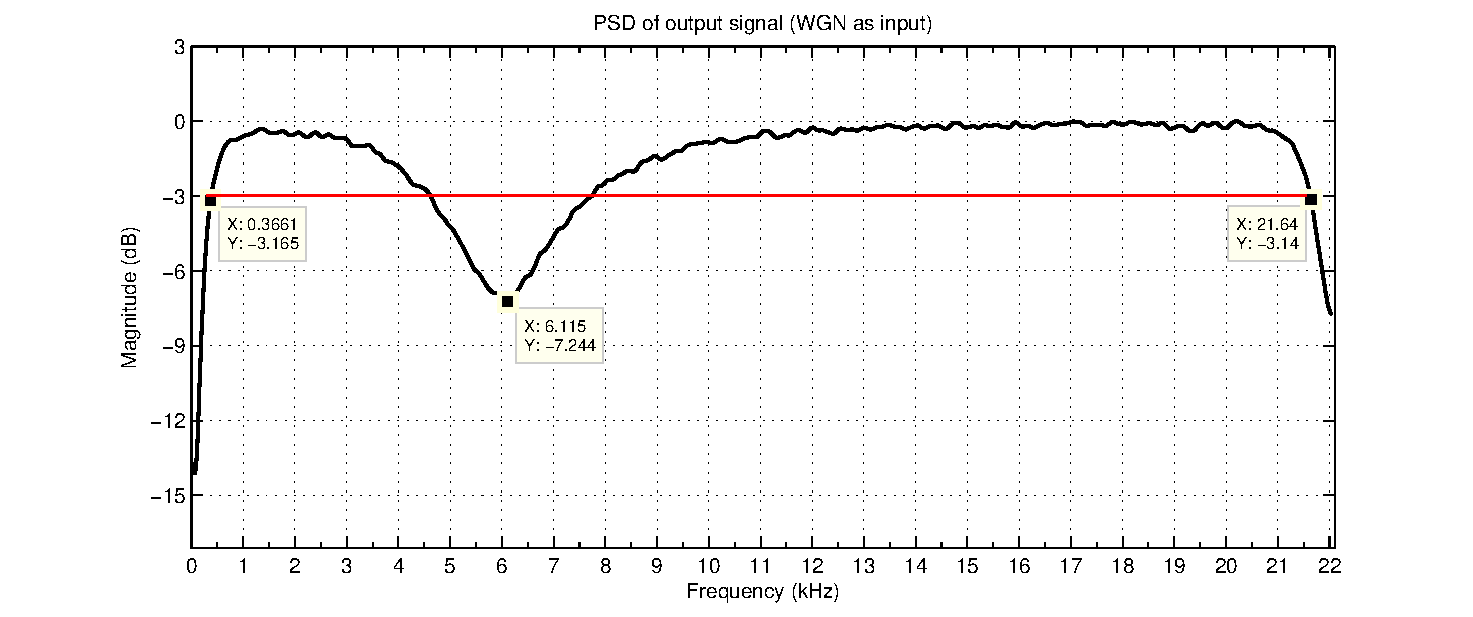
\includegraphics[width=0.7\textwidth]{ChannelResponse.pdf}
\caption[Estimated channel frequency response to WGN]{Estimated channel frequency response to WGN. The measured 3dB bandwidth is 21.27kHz.}
\label{fig:channelresp}
\end{figure}


\subsection{IIR Filters}
Infinite Impulse Response (IIR) filters are recursive structures of a discrete LTI system that can be defined generically in the following form \cite{DSPDiniz}:

\begin{equation}\label{Eq:IIR}
H\left( z \right) = \frac{{\sum\limits_{\ell  = 0}^M {{b_\ell }{z^{ - \ell }}} }}{{1 + \sum\limits_{\ell = 1}^N {{a_\ell }{z^{ - \ell }}} }}.
\end{equation}

 The rational transfer function described in equation \ref{Eq:IIR} implies that the system will have an infinite response when the input is a Dirac impulse. The coefficients from the numerator polynomial correspond to the feed-forward terms, and the ones from the denominator correspond to the feedback terms (see figure \ref{fig:IIRimpl}). IIR filters can be represented in several forms and realisations. However, we generally have to base our design to a given set of initial parameters such as pass-band, stop-band, ripple, or roll-off. The main advantage of these type of filters is that they can efficiently meet a given specification with relative low complexity and efficiency.  Generally, this  computational efficiency is rather large compared to FIR filters described in the next section.
 
  \begin{figure}[H]
   \centering
     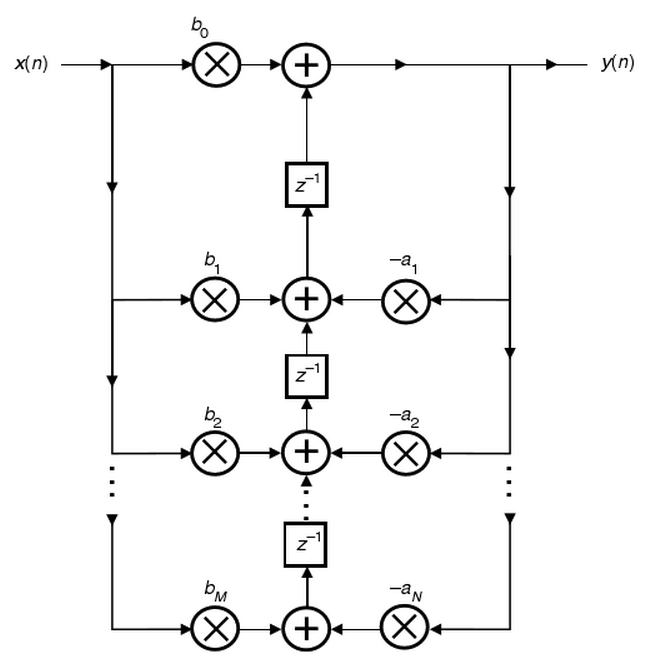
\includegraphics[width=0.5\textwidth]{IIRfilter.png}
     \caption[Shift register implementation of an IIR filter]{Shift register implementation of an IIR filter (Type 2 canonic direct form)\cite{DSPDiniz}.}
     \label{fig:IIRimpl}
 \end{figure}  

\subsection{FIR Filters}
Finite Impulse Response (FIR) filters are non-recursive linear systems that are also widely used in signal processing because of their stability and relative simple implementation. Their transfer function only contains feed-forward terms with coefficients $b_\ell$, directly related with the filter impulse response as follows \cite{DSPDiniz}: 
\begin{equation}\label{Eq: FIR}
H\left( z \right) = \sum\limits_{\ell  = 0}^M {{b_\ell }{z^{ - \ell }}}=\sum\limits_{\ell  = 0}^M {{h_\ell }{z^{ - \ell }}}
\end{equation}

As equation \ref{Eq: FIR} suggest, these kind of filters can be easily designed when we compute the coefficients that characterise the channel impulse response. FIR filters also have good characteristics compared to IIR filters such as linear phase and stability. The biggest problem that we may face when using these designs, is that we need to have a relative high order compared to a similar IIR filter. This adds additional delay to the signal processing and slows down the system. The shift register implementation of a typical FIR filter is depicted in figure \ref{fig:FIRfilter}.
 
  \begin{figure}[H]
   \centering
     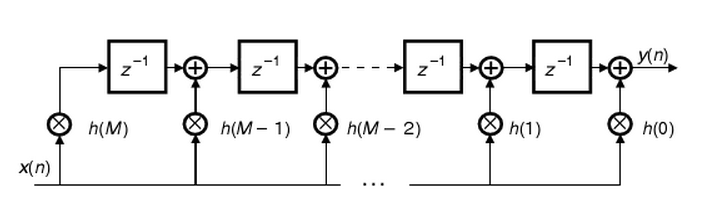
\includegraphics[width=0.8\textwidth]{FIRfilter.png}
     \caption[Shift register implementation for a FIR filter]{Shift register implementation for a FIR filter (Direct form) \cite{DSPDiniz}.}
     \label{fig:FIRfilter}
 \end{figure}  

\section{Channel Coding}
\label{sec:channcod}
The digital signal is subject to diverse perturbations that provoke distortion throughout a non-ideal channel. It is also likely that such distortion  cannot be fully compensated with an equaliser or filter, thus error correcting codes may be implemented. Our channel is bandwidth and power limited. These two parameters together with the noise spectral density will determine the bit-error rate (BER) \cite{HaykinBook}. The channel impairments in our system  result in frequency distortion and ISI. An orthogonal  modulation scheme may be able to mitigate such perturbations. However, it is still likely to have errors at the receiver that can be corrected by adding redundancy to the transmitted signal. This implies that the overall information rate will be decreased when using overheads such as training sequences or error correcting codes.
 
 There are two basic schemes to implement error correction capabilities into our system: error detection/retransmission and forward error correction (FEC) \cite{SklarBook}. In the first scheme, the receiver terminal asks the transmitter to retransmit the data if it detects an error. When FEC is used the receiver tries to recover the signal using the added redundancy. Hence, the detection and retransmission scheme requires a two-way communication contrary to the case of using forward error correction. We focus on the last scheme since our system is only able to send data in one direction. In this fashion, the information message shall be encoded before it is modulated and sent trough the channel (figure \ref{fig:ChanCodTX}). The reverse process is done at the receiver, as shown in figure \ref{fig:ChanCodRX}. The most widely used codes are linear codes, which can be classified into two general forms: block codes and convolutional codes. One of the principal differences between the two groups is that the encoder for convolutional codes has memory elements.
 
  \begin{figure}[H]
  \centering
 	\begin{subfigure}[H]{1\textwidth}
  \centering
     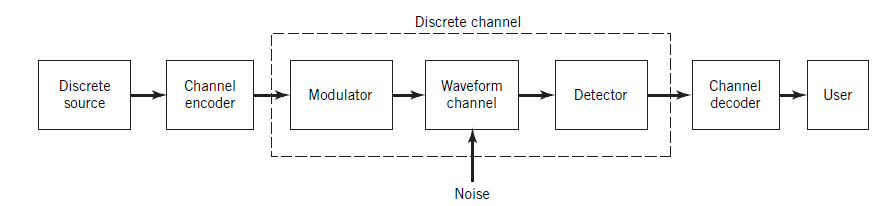
\includegraphics[width=0.8\textwidth]{chancodtx.PNG}
     \subcaption{Transmitter with channel encoder.}
     \label{fig:ChanCodTX}
 
 	\end{subfigure}
 	\quad
 
 	\begin{subfigure}[H]{1\textwidth}
  	\centering
	     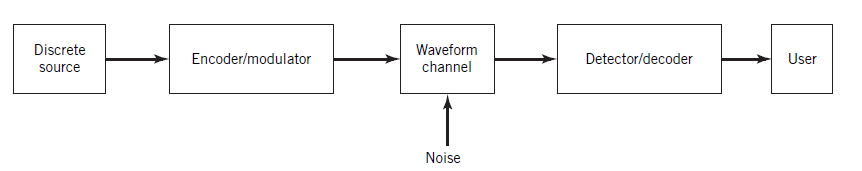
\includegraphics[width=0.8\textwidth]{chancodrx.PNG}
     \subcaption{Receiver with channel decoder.}
     \label{fig:ChanCodRX}
  	\end{subfigure}
     \caption[Digital communication system with forward error correction]{Digital communication system with forward error correction \cite{HaykinBook}.}
     \label{fig:ChanCoding}
 \end{figure}
 
 
 \subsection{Block Codes}
  
 In general, binary block codes  are parity check codes that can be characterised by the parameters $(n,k)$. In this notation, $n$ represents the number of encoded bits and $k$ is the number of information bits. We define the ratio $k/n$ as the rate of the code. The mapping from the set of $M=2^k$ information sequences of length $k$ can be represented by a $k\times n$ generator matrix, conventionally denoted as $\bf{G}$. Therefore, we can write the encoded sequence $\bf{c}$ (of length $n$) in matrix form as follows:
\begin{equation}
 {\bf{c}} ={{\bf{u}}}{\bf{G}}
 \end{equation}
The vector  $\bf{u}$ denotes the information sequence (of length $k$), and the row vectors of $\bf{G}$ determine the basis of a non-unique vector space. When $\bf{G}$ has the form ${\bf{G = }}\left[ {{{\bf{I}}_k}{\bf{|P}}} \right]$, we could find a parity matrix ${\bf{H = }}\left[ {{{\bf{I}}_{n - k}}{\bf{|}}{{\bf{P}}^T}} \right]$ that would lead us to decode the original data\cite{SklarBook}. These codes are mainly used for hard-decision decoding with a built-in algebraic structure based in the properties of finite fields. There exist a variety of block codes called Long-Density Parity-Check Codes (LDPC) that can achieve performance very close to the channel capacity.  


 \subsection{Convolutional Codes}
 Convolutional codes are linear codes that are generated by passing the information sequence through a shift register. They can be described by some encoding function $G({\bf{u}})$, such that ${\bf{c}}=G({\bf{u}})$. The encoder outputs at any given time will only depend on the inputs. The number of output bits for each $k$-bit input is a sequence of length $n$. We also need to define the parameter $K$ as the code constraint length, which represents the number of stages (of $k$-bits) in the encoder. 

One possible method to describe a convolutional code is by giving its generator matrix. Nevertheless, such matrix would be semi-infinite since the input sequence can have any arbitrary length\cite{Proakis}. A different method to describe a convolutional code comes from the fact that each of the output sequences can be interpreted as the convolution of the input sequence with a binary filter defined by its ``impulse response" or generator polynomial\footnote{Since we are using binary arithmetic operations, the polynomials are equivalent to the filter taps. They are typically given in the octal form.}, denoting the links between the input, output and shift registers. A typical shift register implementation of such codes is shown in figure \ref{fig:convCodeImp}.
 
 
  \begin{figure}[H]
   \centering
     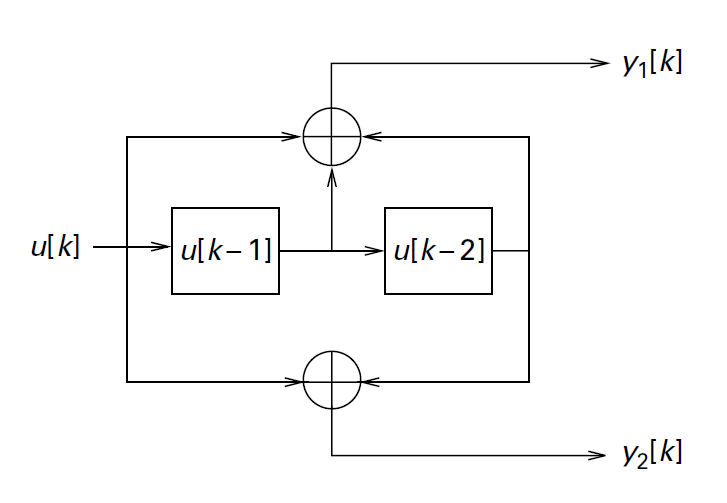
\includegraphics[width=0.4\textwidth]{convCode.PNG}
     \caption[Shift register implementation of convolutional encoder]{Shift register implementation of convolutional encoder with generator polynomials $[7,5]$ \cite{Madhow}.}
     \label{fig:convCodeImp}
 \end{figure}  
 % ConvCodesTut

 The most common implementation for the decoding is the Maximum Likelihood Viterbi algorithm. In this algorithm, the decoder examines an entire sequence and computes a metric on every state based on each of the possible paths (branches) that the sequence might have followed. The branch with the higher metric is kept in every state, and the resulting path is the decoded sequence. The most common used metric is the Hamming distance \cite{ConvCodesTut}.
 
 Convolutional codes may be used as a building block for turbo-codes, which can perform very close to the channel capacity as well as LDPC codes do. The major disadvantages for those two approaches are the relative complexity and hard processing that are required to achieve a good performance. 

\section{Channel Capacity}

\textcolor{red}{Theory}.\\


For any channel there is a maximum achievable rate called the channel capacity. In the case of a real valued AWGN channel with bandwidth \(B\) this capacity can be shown to be:

\begin{equation}
\label{Eq:awgn_capacity} C = B \log_2(1+\text{SNR})\text{                [bps]}
\end{equation}

% % % % % % % % % % % % % % % % % % % % % % % % % % % % % % % % % % % % %
% % % % % % % % % % % % % % % % % % % % % % % % % % % % % % % % % % % % %




\chapter{Android Prototype}
\label{chap:App}
Our aim is to build a full digital communication system that uses a pair of Android phones as terminals. The communication between them is done with an audio cable that serves as the channel together with the devices' sound cards. The implementation consists of two modes: off-line and real-time. We define off-line and real-time as follows. Assume that the file size is $F$ (bits) and the data-rate $C$ (bps). The transmitter is allowed to transmit signals during $F/C$ seconds. In off-line mode, the receiver should be able to decode the signal within 100 seconds using the received signal downloaded from the phone using MATLAB. In real-time, the receiver should finish decoding within $0.5\times F/C$ seconds after the transmitter has finished sending the data. The file should have a size between 100 and 1000 bytes \cite{EQ2440ProjectDescription}.

The advanced specification requires a data-rate of 32 kbps in real-time and 128kbps in off-line mode. In real-time the system should be able to transmit file sizes up to at least 10kB.


\section{Software and Hardware}


\textbf{Used Hardware}
\begin{itemize}
\item Samsung Galaxy S3 (GT-i9300) phones with Android 4.2.1.
\item 3.5mm audio cable {\color{Black}\footnote{The audio cable is modified so as to have the audio input in one end linked to the audio output in the other extreme. The communication is in one direction only.}}.
\item Dell PC's with Windows 7.
\\

\textbf{Used Software}
\item MATLAB R2013b 
\item Android Developer Tools IDE (Eclipse) with  API for Android 4.1.2. 
\item Git source code manager software for Windows.

\end{itemize}


\section{Android FrameWork}

Framework is an Android application developed by Martin Ohlsson and Per Zetterberg which has been designed as the basis for our project, and will serve as support for our software implementation in real-time. The JAVA based implementation contains functions, methods and classes that enable the control and initiation of various sensors of the Android phone (e.g. microphone, camera, speakers, among others). In addition, it has an embedded  Guided User Interface (GUI) and a number of valuable built-in features that allow us to develop our implementation of a communications system without going to deep into software designing. \\

Figure \ref{fig:FrameWorkPicture} illustrates a simplified UML\footnote{The Unified Modeling Language (UML) is a general-purpose modeling language in the field of software engineering, which is designed to provide a standard way to visualize the design of a system \cite{UMLref}. } diagram of the completed FrameWork, showing the classes' relations and emphasising the functions that were added. That is the case of classes like \texttt{Complex.java}, which allows us to use and handle complex numbers in the application. The class \texttt{StudentCode.java} (part of FrameWork) is the core of our system and thus, the basis of our implementation. 




 \begin{figure}[H]
  \centering
    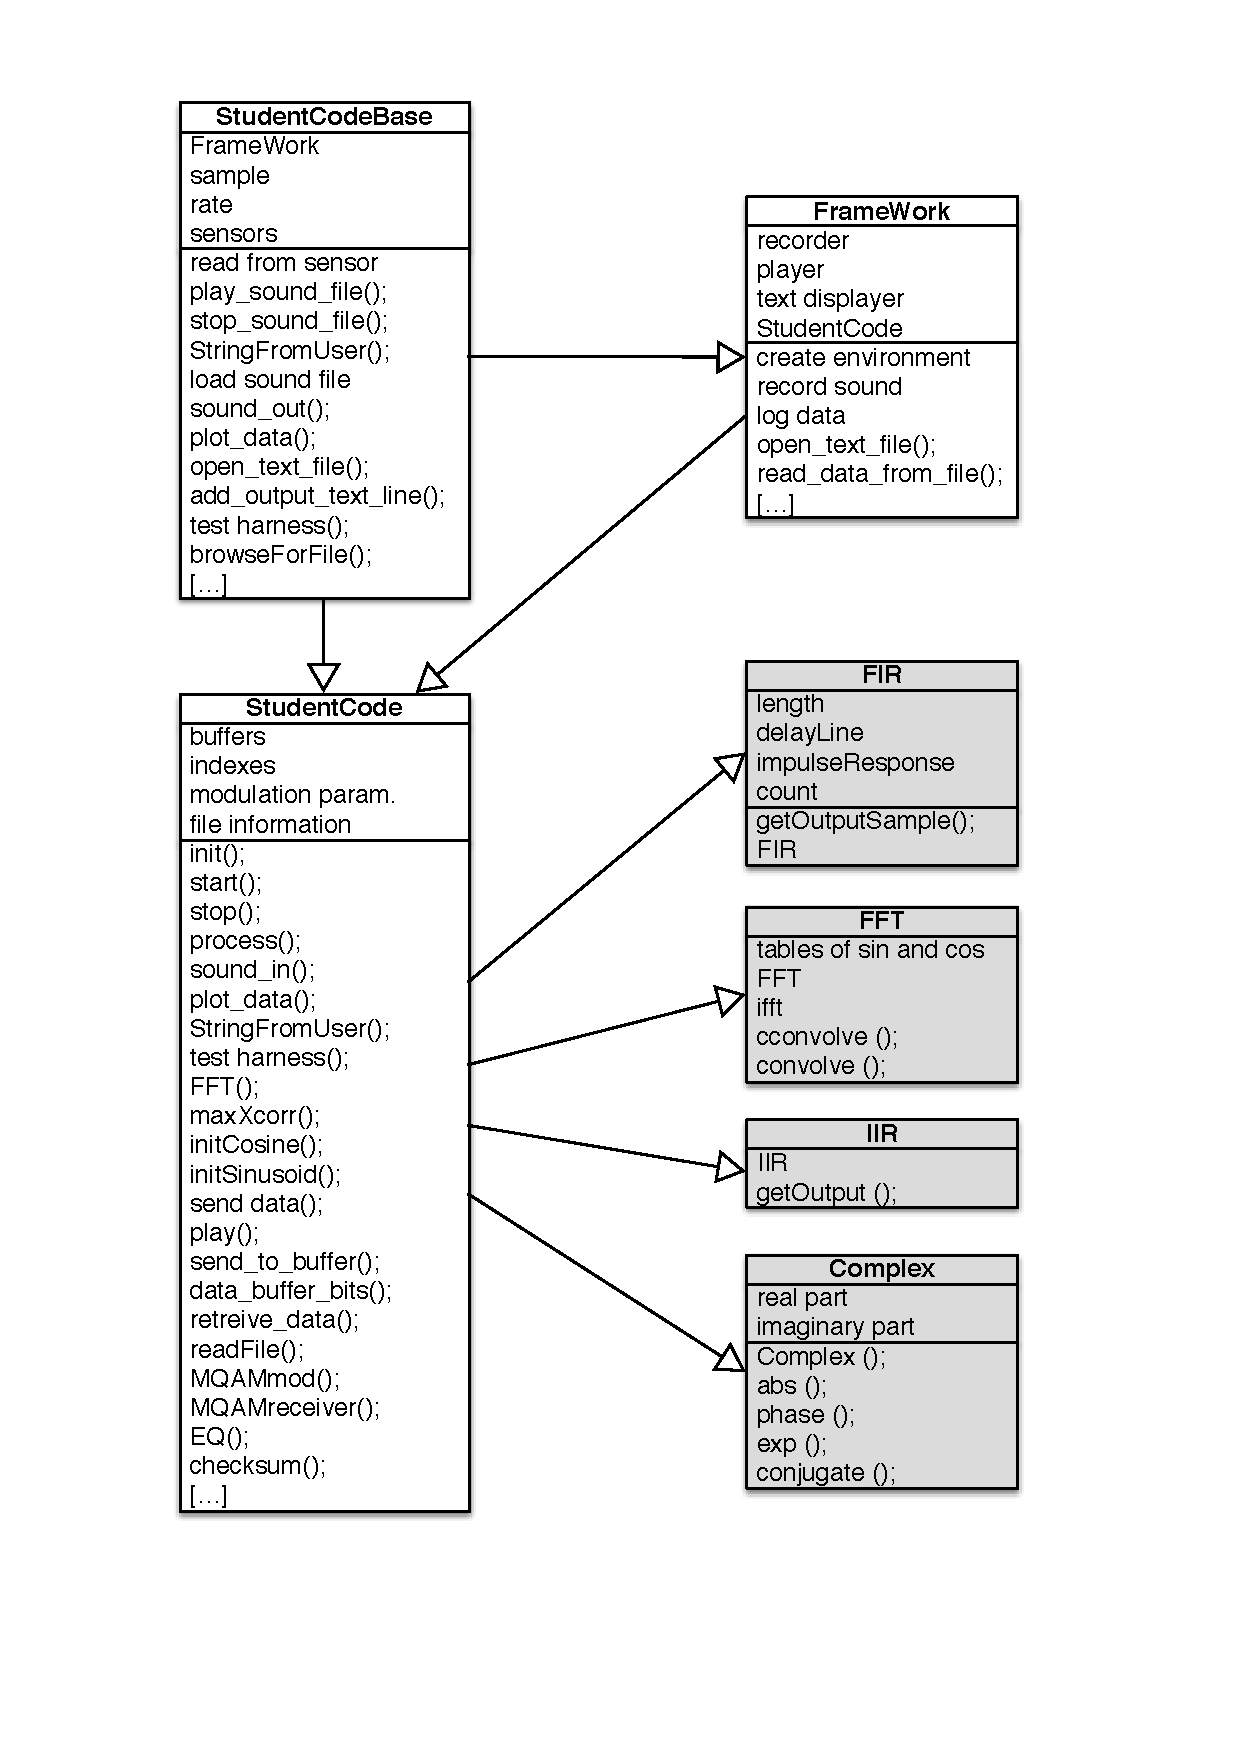
\includegraphics[width=0.6\textwidth]{UmlScheme.pdf}
    \caption[Simplified UML diagram of Application FrameWork]{Simplified UML diagram of Application FrameWork. }
    \label{fig:FrameWorkPicture}
\end{figure}



\section{Application Implementation} %Change the name for something else

The schematic of the file transfer application in form of system blocks is illustrated in figure \ref{fig:SchematicsSystem}. There are two basic functions in the transmitter, convert the file into a binary stream (denoted as Encode File), and the modulation stage (Modulate Data). The receiver does the reverse process to recover the original file. 

 \begin{figure}[H]
  \centering
    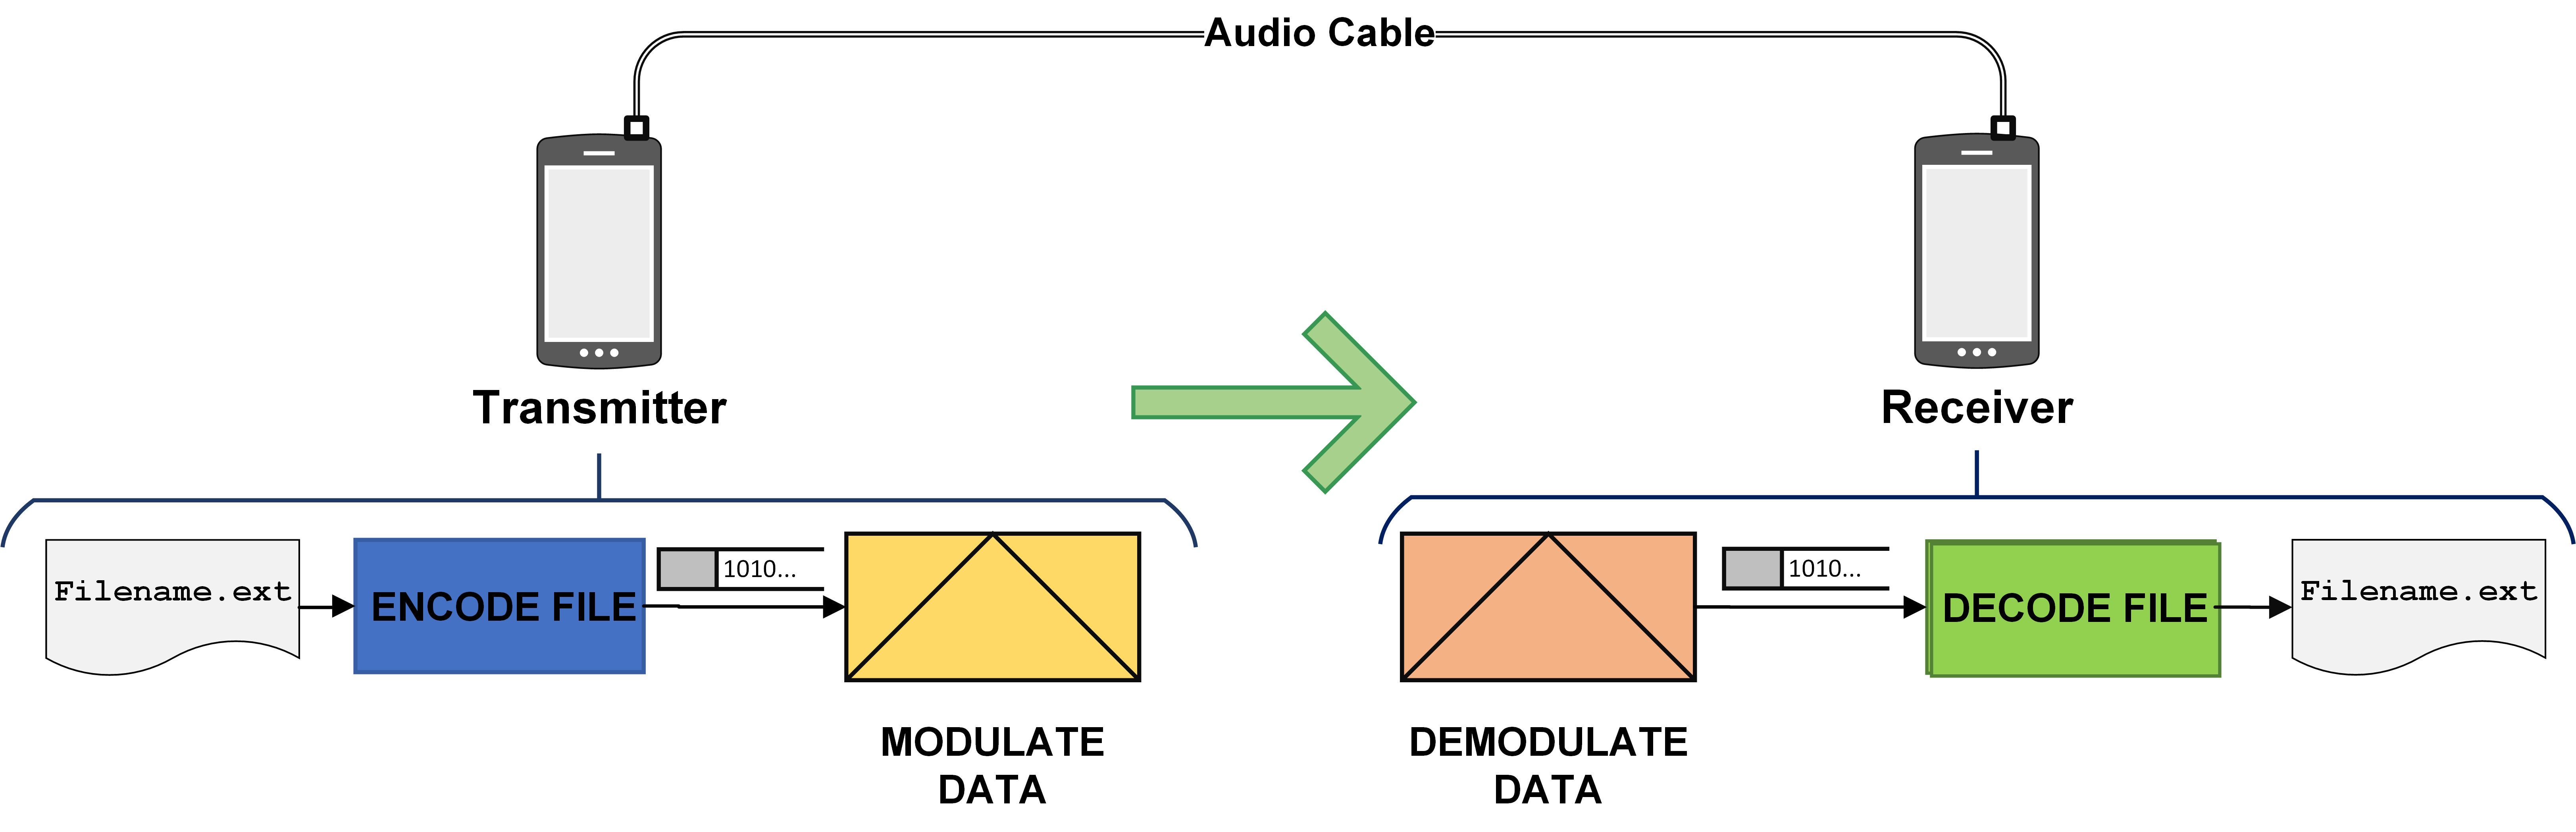
\includegraphics[width=1\textwidth]{FullSystem.png}
    \caption[Schematic of the file transfer system]{Schematic of the file transfer system.}
    \label{fig:SchematicsSystem}
\end{figure}

The functions described above are embedded in the modes \emph{TX} and \emph{RX}, which can be chosen from the built-in menu depicted in figure \ref{fig:menuoptions}. When \emph{TX} is pressed, the user has the option to select the file that is going to be sent. After the file is selected, the application reads the file from the phone's file system and starts the encoding process and modulation afterwards. Then, the resulting signal is sent through the channel. The transmitting phone changes to an idle state after the transmission is complete. Meanwhile, the receiving phone has to be set in \emph{RX} mode. When the signal is detected, the application starts to process the file and does the demodulation after receiving the data. The file is reconstructed, verified against errors, and stored in the receiving phone's internal file system. The user now has the option to open the received file, select a different mode, or start the process all over again. Furthermore, the \emph{Input String} option allows the user to input text and generate a simple text file that is stored in the phone with the name \texttt{MessageFromUser.txt}. Finally, the \emph{Quit} option, closes the application. 


 \begin{figure}[H]
  \centering
    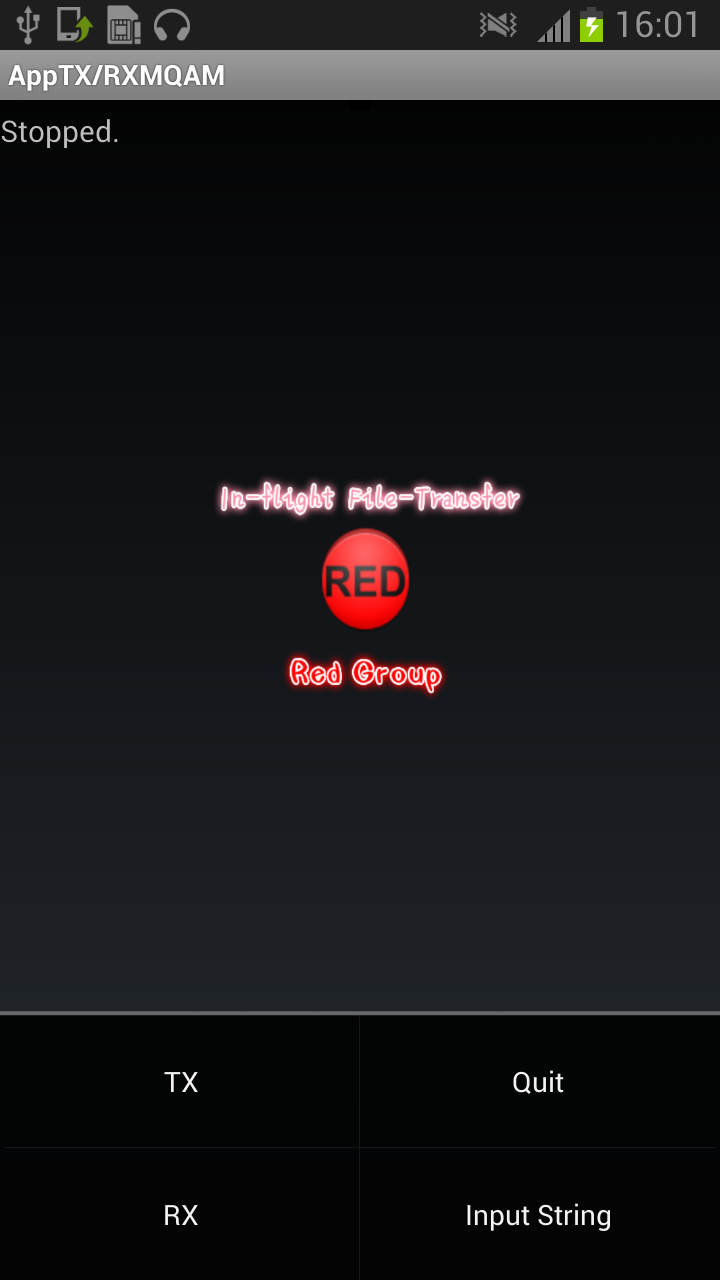
\includegraphics[width=0.3\textwidth]{menuoptions.png}
    \caption[Start Menu options]{Start Menu options.}
    \label{fig:menuoptions}
\end{figure}



\subsection{Transmitter}

A flow diagram of the transmitter main functions is illustrated in figure \ref{fig:TXclientFull}. The transmission process begins when the user press the option \emph{TX}. Then, the application calls the method \emph{Browse For File} that shows a GUI in which the user selects a file from the phone's file system. The following process is \emph{Generate Bitstream}, that builds the binary sequence that is going to be modulated. Such block consists on the sub-processes shown in figure \ref{fig:TXclientRecFile}. The first sub-process to generate the bitstream is computing the file checksum and store it in a variable. Next, the data is stored in an array of bits that is concatenated with the remaining headers (guard bands, training sequence, size of file, title of file and checksum value). The length of the headers has been optimised to have a solid performance and it is detailed in table \ref{table:headers}. 

\begin{table} [h]
\centering
\begin{tabular}{lc} 
\hline
\bf{Header}	& \bf{Length}\textnormal{[bits]}    \\
\hline
\emph{Name of file}       & 768              \\  
\emph{File size}        & 768              \\   
\emph{Checksum}        & 768              \\   
\hline
\emph{Initial guard band}      & 3120           \\   
\emph{Training sequence}    & 1200              \\
\emph{Final guard band}     & 3120              \\
   
  
\hline
\end{tabular}
\caption[Length in bits for bitstream headers]{Length in bits for bitstream headers.}
\label{table:headers}
\end{table}

After the bitsteam is correctly generated, the \emph{Modulate Bitstream} process takes place. Such process will be further described in section \ref{sub:MQAMtx}. Finally, the modulated samples are sent to the \emph{Play Audio} method, which plays the buffered data as sound.
 


%\textcolor{red}{When, the user chooses a file which is opened and read as an array of bytes. These bytes are the n converted to a binary stream of ones and zeros, which are modulated with a given scheme along with a guard band and training sequence. The bits are then, modulated with a given scheme along with the guard-band and the training sequence. The total modulated signal (information data, guard band, training sequence and headers) is sent to the audio buffer, that plays the sound through the channel. The headers include the name, size and extension of the file along with a checksum value.}

 \begin{figure}[H]
 \centering
 \begin{subfigure}[t]{.7\textwidth}
 \centering
    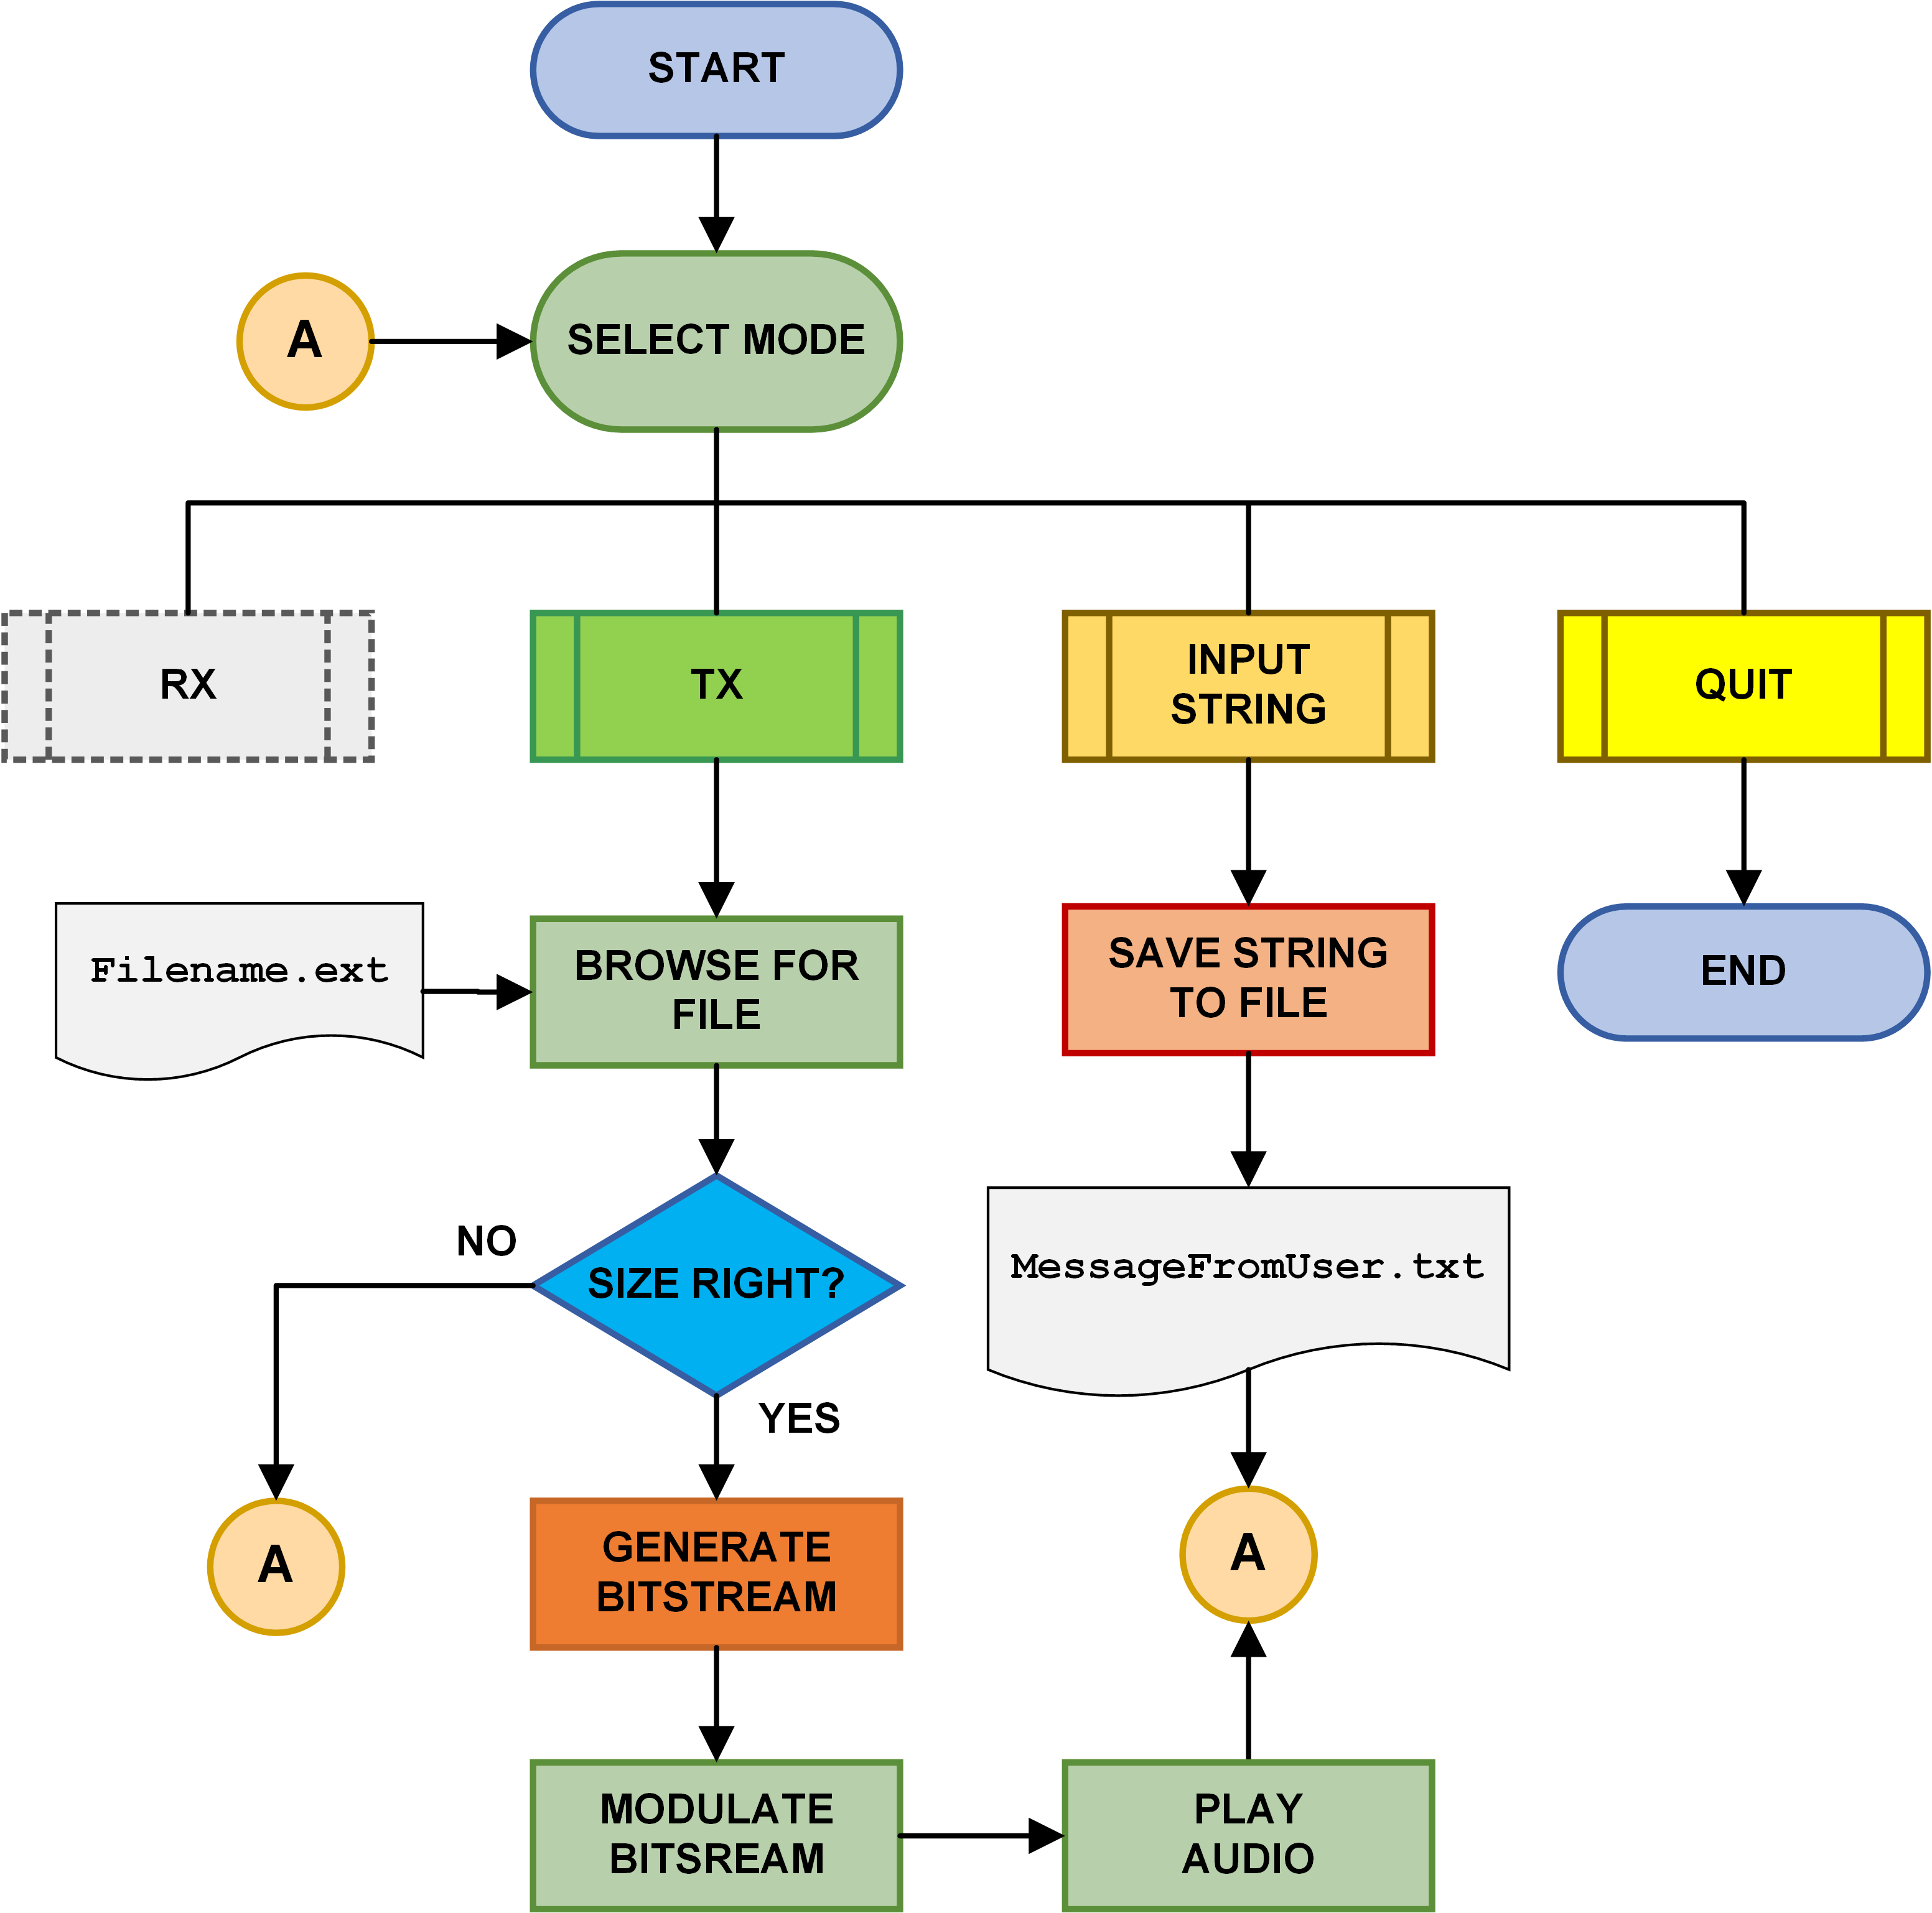
\includegraphics[width=0.8\textwidth]{TXschem.png}
    \subcaption{Transmitter processes.}
    \label{fig:TXclientFull}
    \end{subfigure}%
 \begin{subfigure}[t]{.3\textwidth}
  	 \centering
      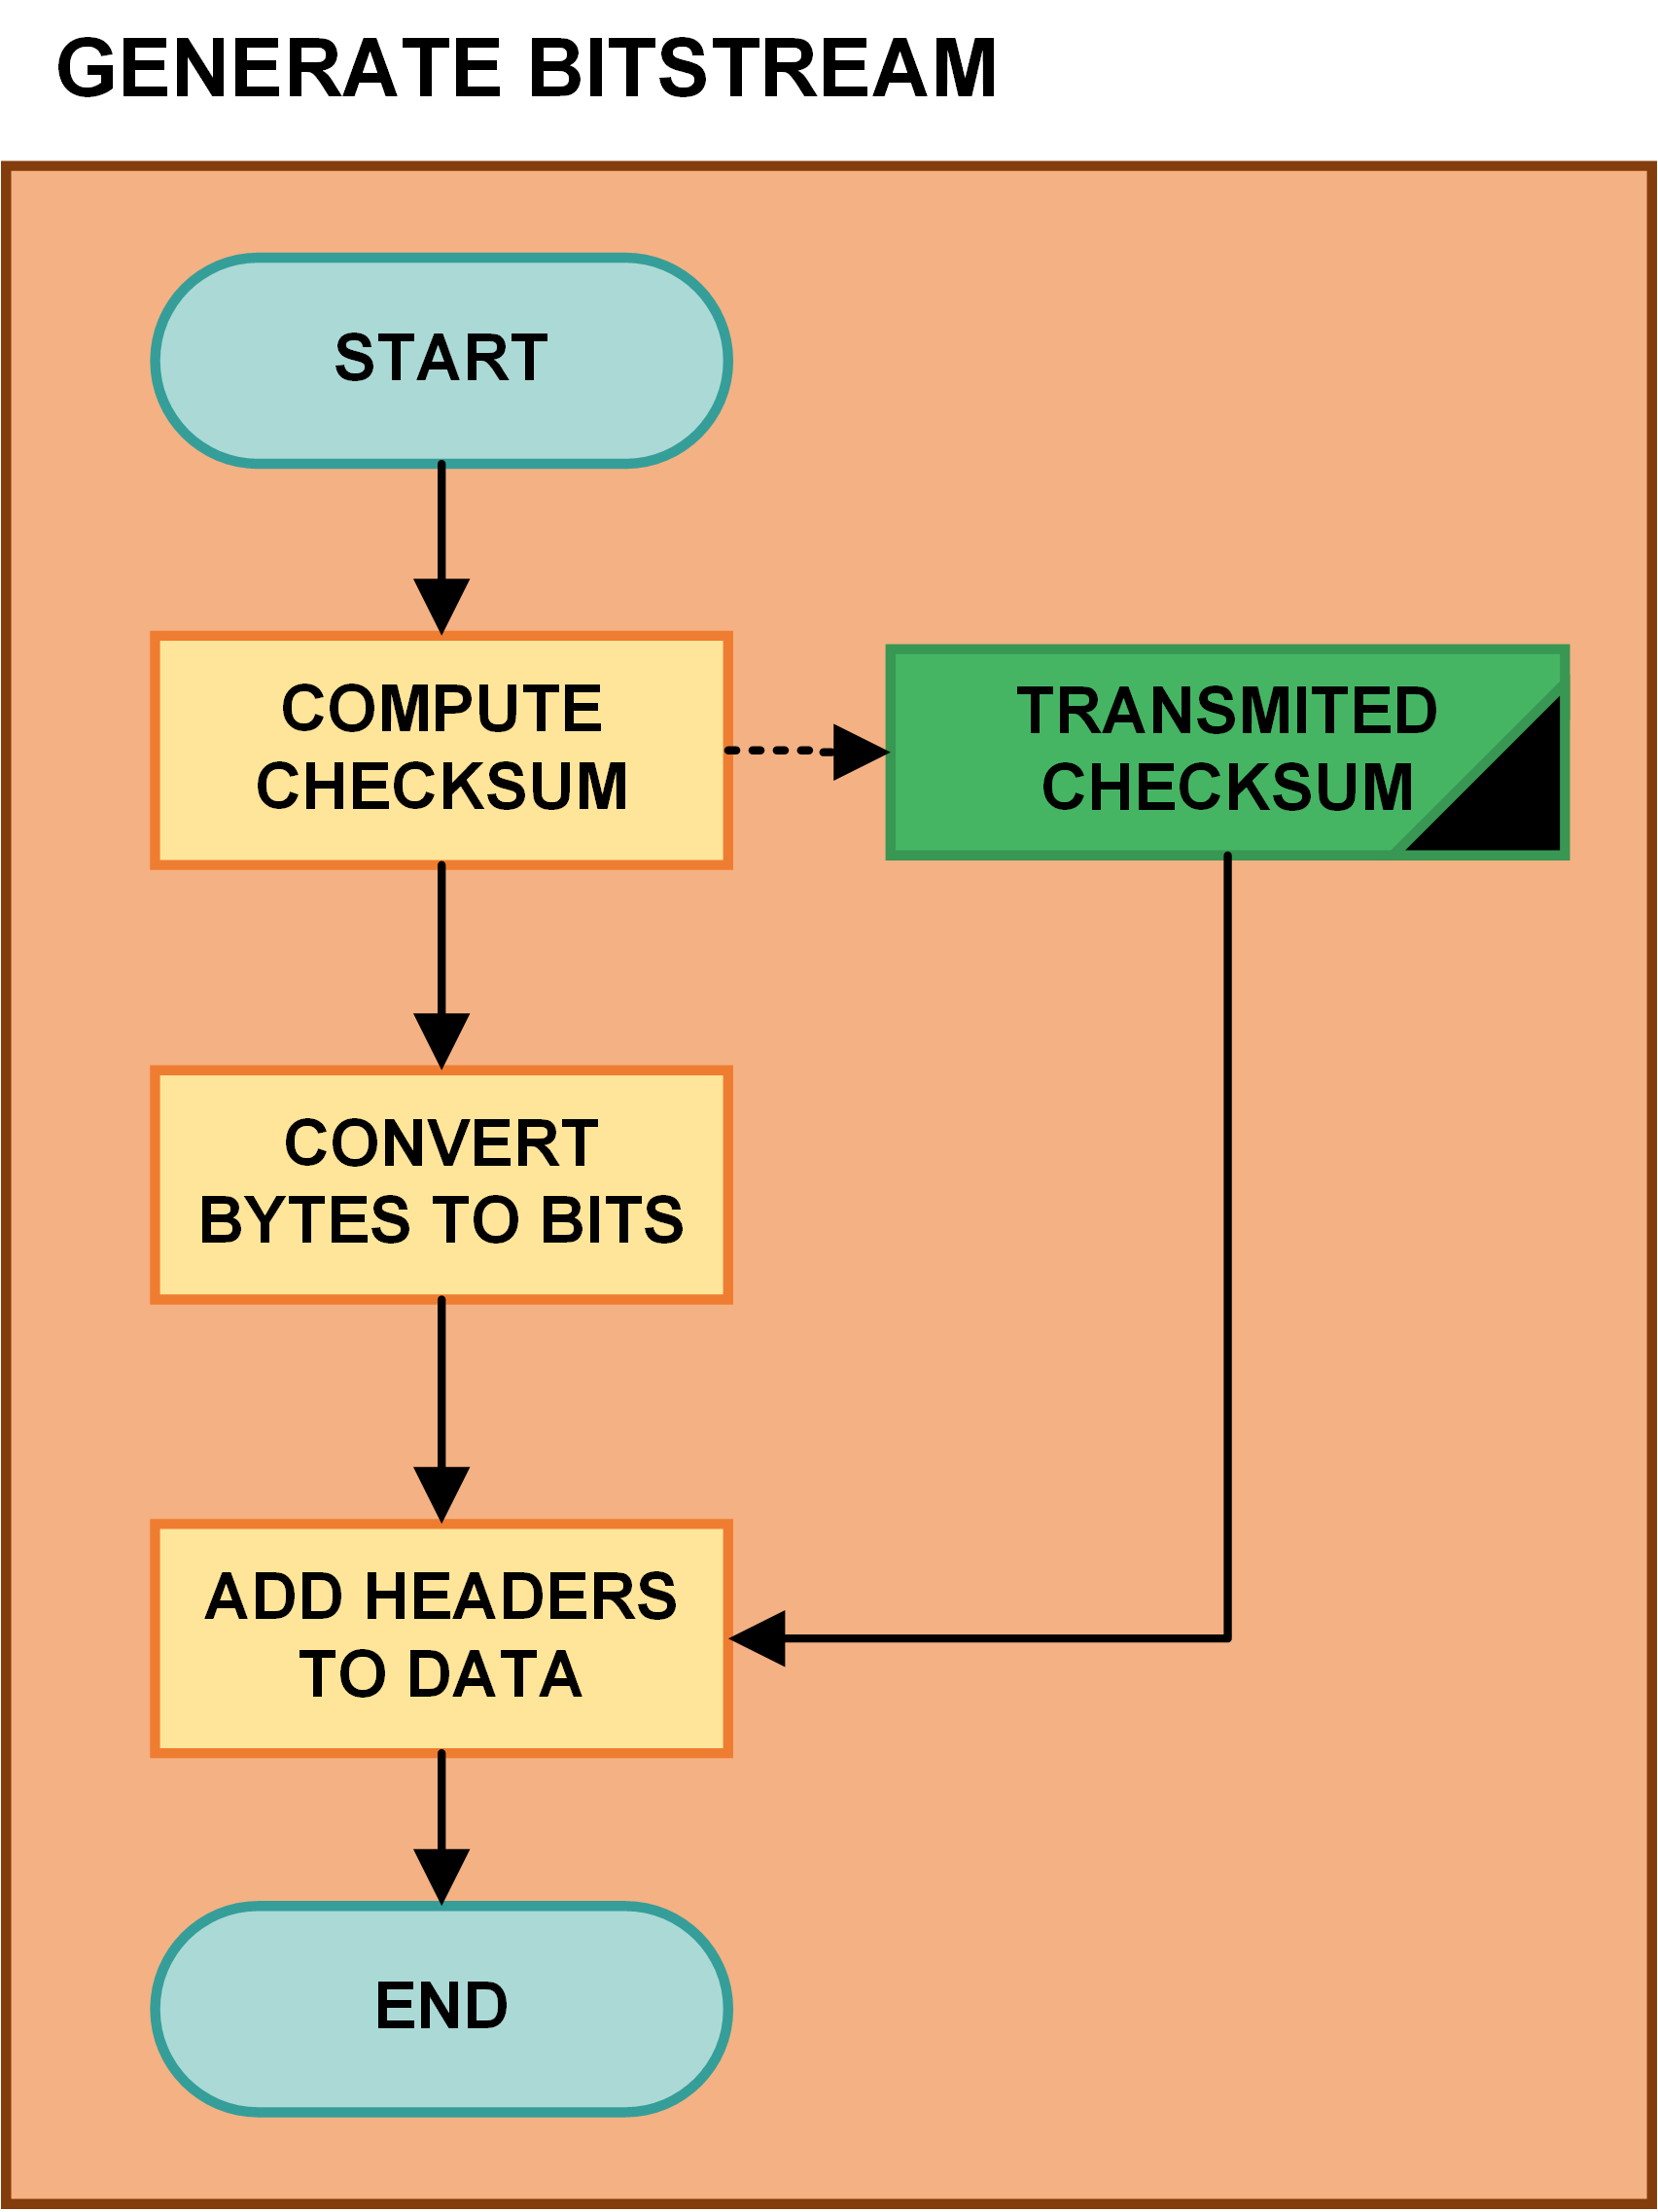
\includegraphics[width=0.8\textwidth]{schemGenBS.png}
      \subcaption{Generate Bit-stream sub-processes.}
      \label{fig:TXclientRecFile}
   \end{subfigure}
    \caption[Transmitter client flow diagram]{Transmitter client flow diagram.}
     \label{fig:TXclient}
 \end{figure} 




%\clearpage
\subsection{Receiver}
The flow diagram of the processes that are needed to receive a file is illustrated in figure \ref{fig:RXclientfull}. When \emph{RX} is pressed, the phone starts to "listen" continuously to the audio input and waits for a signal threshold to be surpassed. If the threshold condition is fulfilled, the \emph{Receive Signal} process takes place. Such process, stores the received signal in a buffer until the received samples fall below the threshold limit. The block of buffered data goes next to the \emph{Demodulate Data} function. This part runs the process that will be detailed in section \ref{sub:MQAMrx}. If the data is correctly demodulated, we now have the process \emph{Reconstruct File} depicted in figure \ref{fig:RXclientRecFile}. This process begins extracting the headers of the received data (e.g. \emph{Retrieve Data}) and store them in variables that will be helpful to reconstruct the file. The next sub-process is to reconstruct the file according to its headers. The last sub-process is \emph{Compute Checksum} of the received data. If the data is corrupted, an error flag is triggered; otherwise, the file is stored in the phone's file system. Finally, the user now has the option to either open the received file or return to the \emph{Select Mode} state.

       
%\textcolor{red}{
%In figure \ref{fig:RXclient} a flow diagram of the receiver functionalities is illustrated, along with a diagram of how the received file is reconstructed. The application starts listening and verifies if there are any samples above the detection threshold. If the samples are below the threshold, it is considered only noise. Otherwise, the application starts buffering the input sound until the transmission is completed or the buffer is full. \textcolor{red}{If the buffer is full, a new one is created.}
%The received data is then processed and synchronised by correlating with a training sequence. Then the application applies the detection algorithm retrieving the sent bitstream. Such data is then processed and the name, size, data and checksum value of the selected file are retrieved. The application uses this information to reconstruct the original file before saving it to the phones SD-Card. The user now has the option to either open the received file or return to the idle state. }
 \begin{figure}[H]
 \centering
 \begin{subfigure}[t]{.7\textwidth}
 \centering
    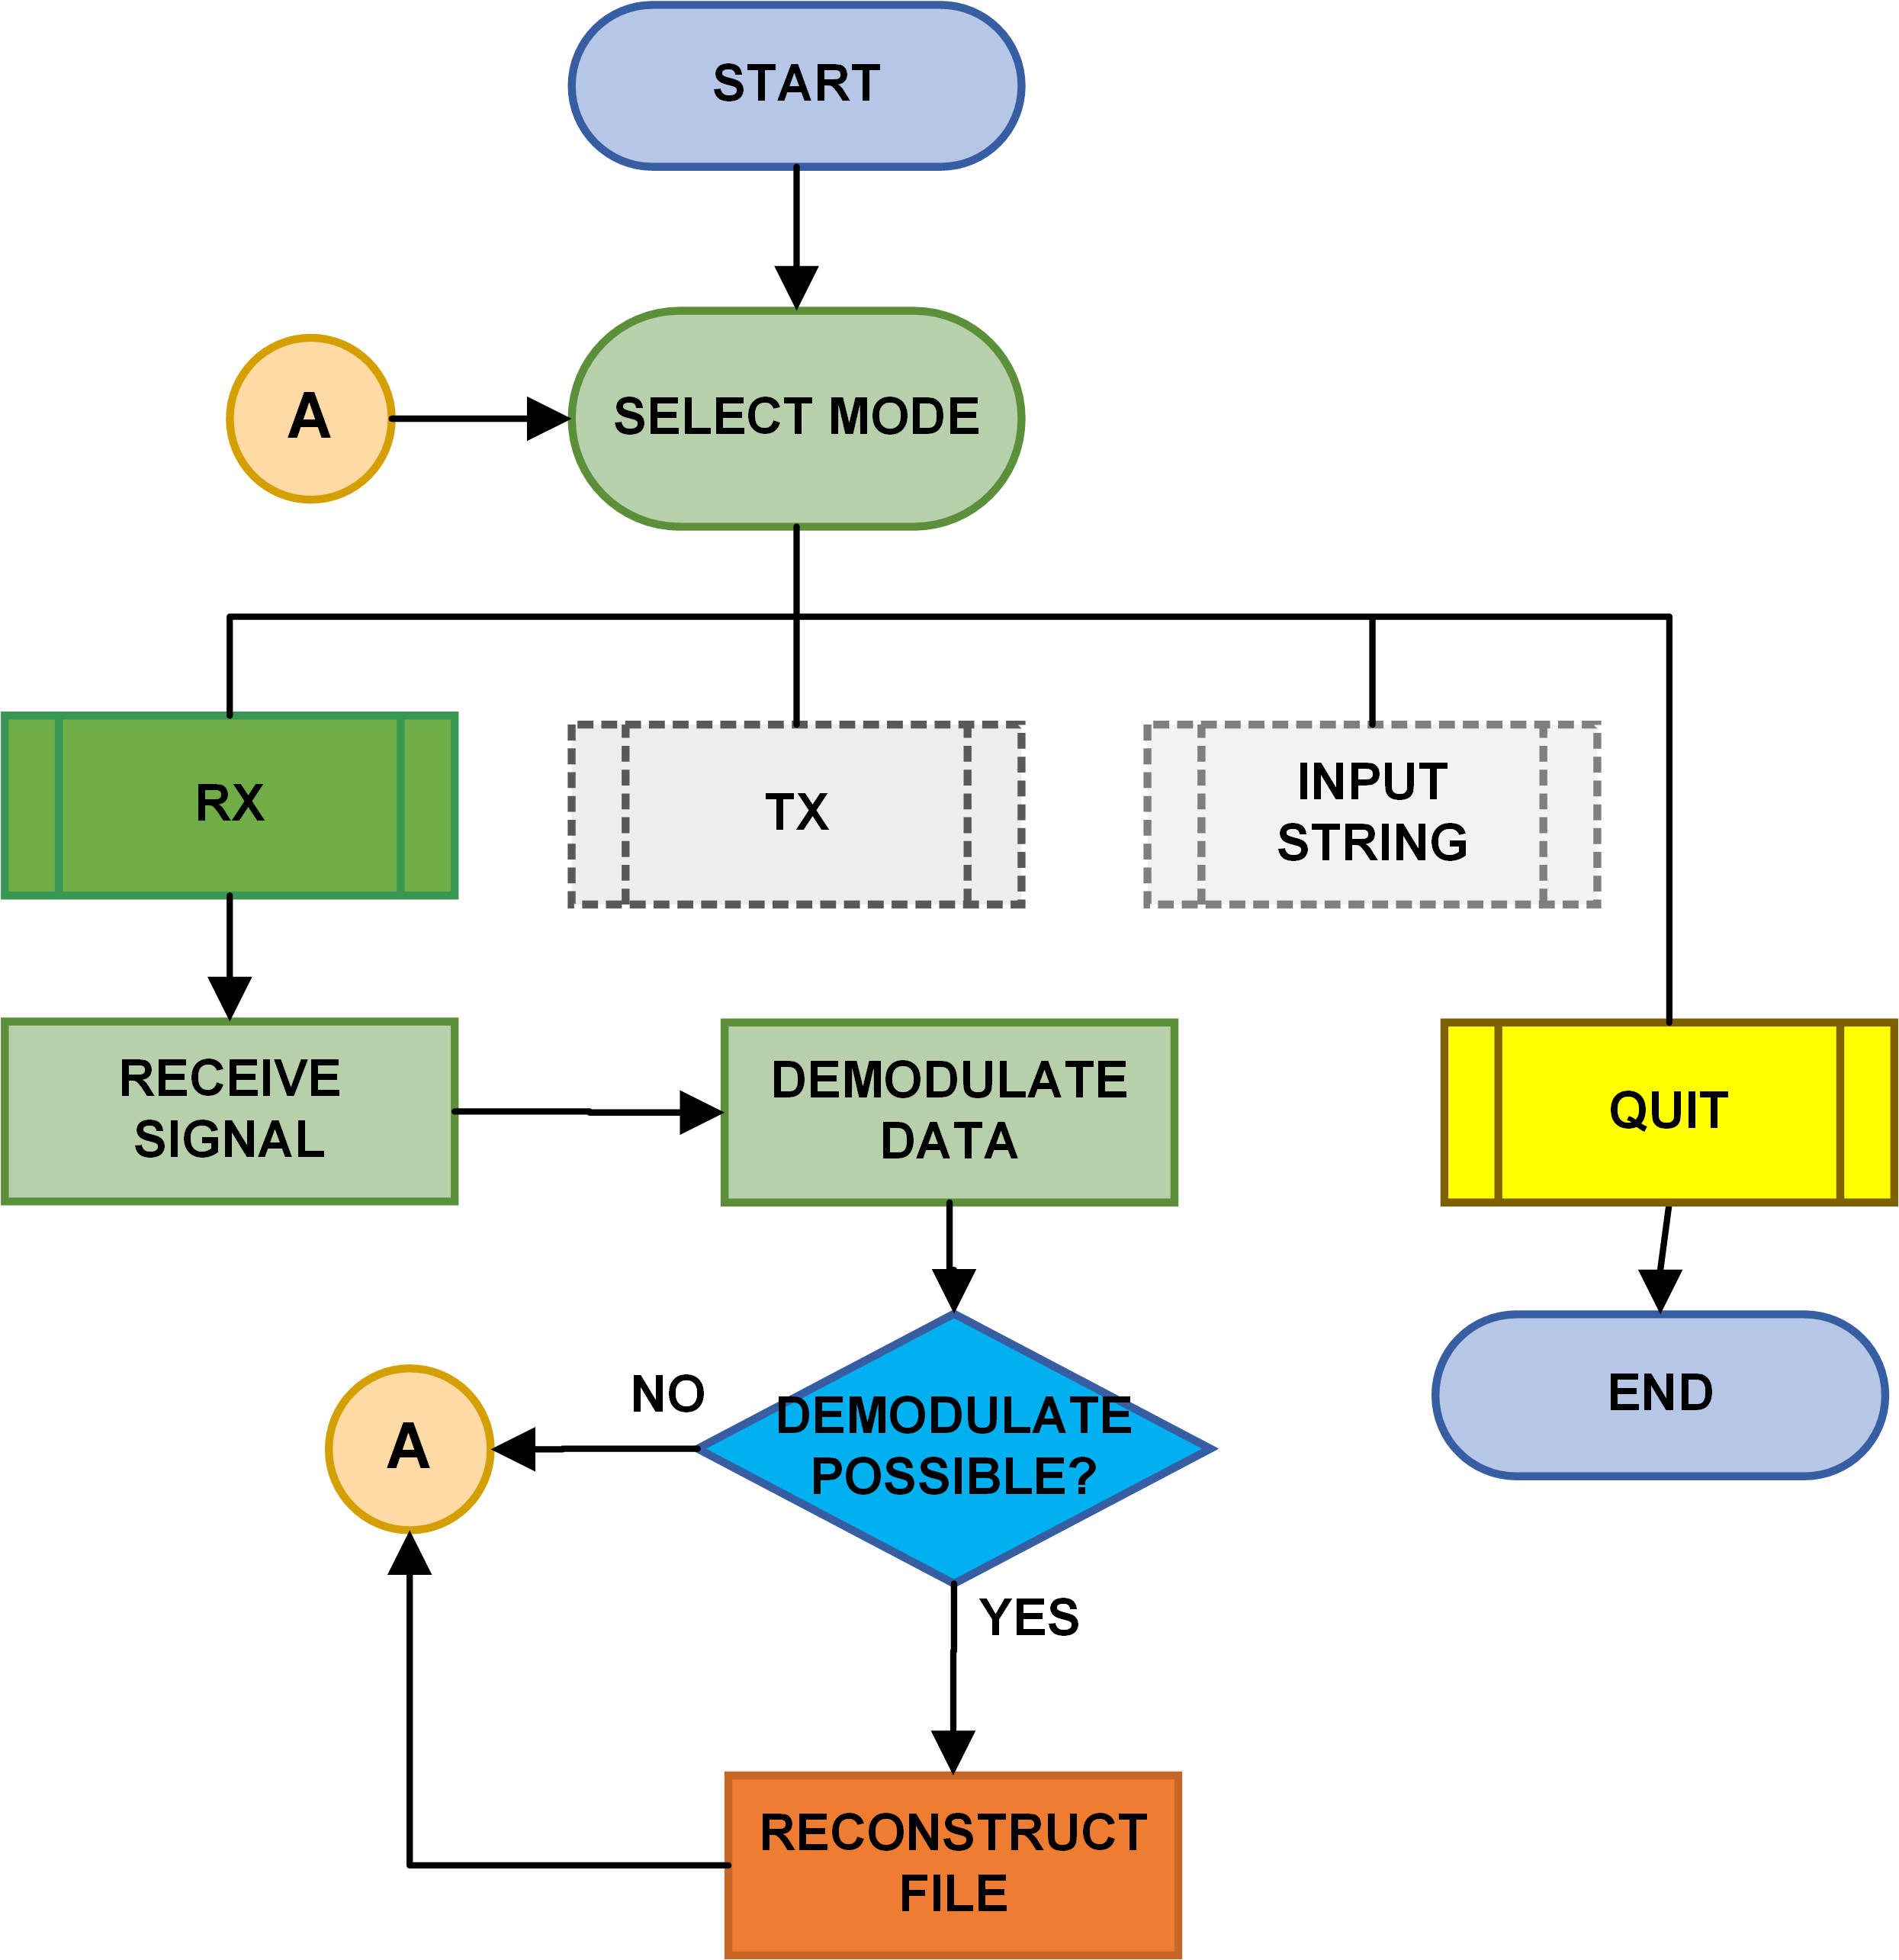
\includegraphics[width=0.8\textwidth]{RXschem.png}
    \subcaption{Receiver processes.}
    \label{fig:RXclientfull}
    \end{subfigure}%
 \begin{subfigure}[t]{.3\textwidth}
   \centering
      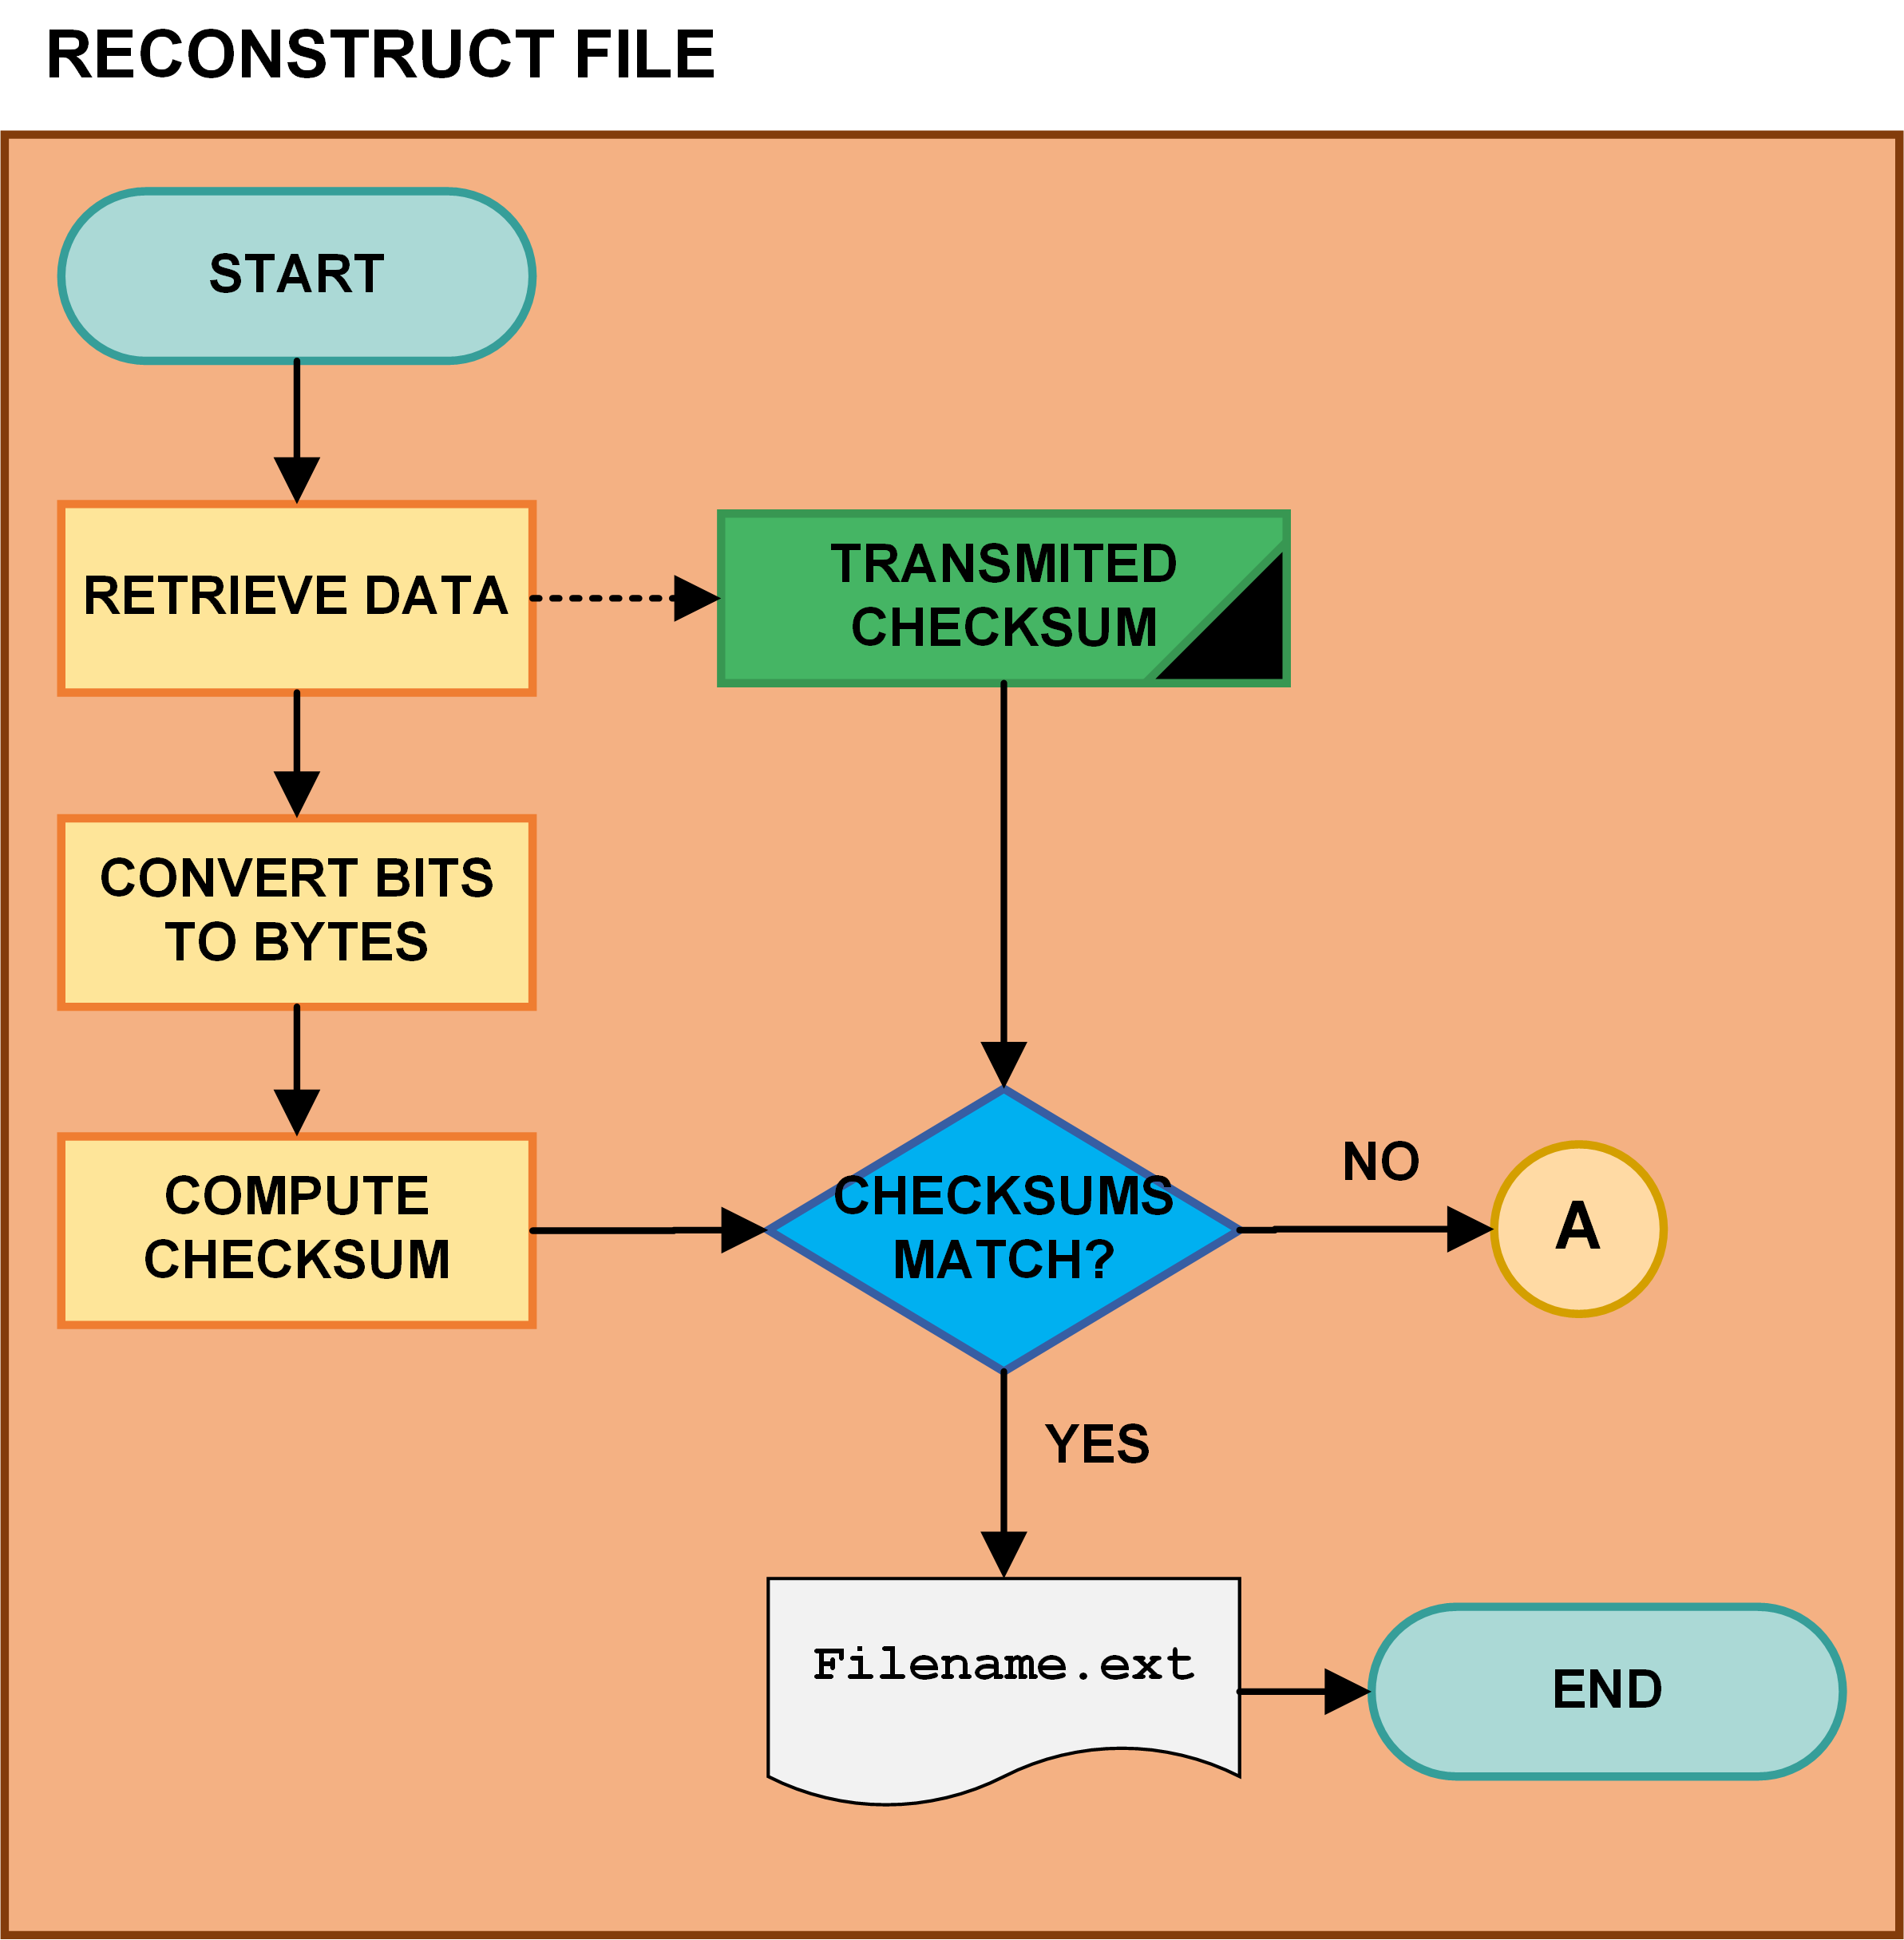
\includegraphics[width=1\textwidth]{RXreconstructSchem.png}
      \subcaption{Reconstruct file sub-processes.}
      \label{fig:RXclientRecFile}
   \end{subfigure}
      \caption[Receiver client flow diagram]{Receiver client flow diagram.}
      \label{fig:RXclient}
 \end{figure} 
 
\subsection{Checksum}
\label{subsec:Checksum}

The checksum used in our application is the internet checksum which is widely used in standard internet protocols \cite{Checksumref1}. Its implementation consists on taking a vector of bytes as input and performing the following operations:
 
\begin{enumerate}
  \item Compute ones complement sum of adjacent octets by combining them to one 16-bit integer over all the concerned bytes.
  \item The checksum field is cleared and the value stored here is the ones complement of the final sum computed in the step above.
  \item To check the checksum value. Steps one and two are performed over the same set of bytes. If the result are all one bits, the checksum succeeds; otherwise, it fails.
\end{enumerate}
 
Note that ones complement is the bitwise NOT operation. The checksum value is computed for our information data and is then added as a binary header to be sent through the channel. This value is retrieved at the receiving phone. In order to make sure that the file is not corrupted during the transmission, the checksum is computed once more to the retrieved data and compared with the transmitted signal. The checksum is able to detect one or more errors in the transmission and it has a length of 768 bits (96 bytes). In case the number of errors was larger than this amount and the checksums were equal, we may have a wrong decision. However, this is highly unlikely.
 
% % % % % % % % % % % % % % % % % % % % % % % % % % % % % % % % % % % % % % % % % % % % % % % % %
% % % % % % % % % % % % % % % % % % % % % % % % % % % % % % % % % % % % % % % % % % % % % % % %


\chapter{Method}
\label{chap:method}
In chapter \ref{chap:Background} we introduced the fundamentals of each modulation scheme. Now we focus on the development of the algorithms used in our implementation. The main part are the modulation, demodulation, channel equalisation and coding techniques. 

\section{M-FSK System}

The first design is based on an FSK system with off-line and real-time implementations. The system used is a M-ary FSK system (2-FSK is used for synchronisation and 4-FSK is used for data modulation) with orthogonal envelopes to improve the bandwidth efficiency of the MFSK system. 

\subsection{M-FSK Transmitter}

With a 4 FSK system it is possible to transmit $\log_2(4)=2$ bits per symbol. It is then necessary to compute the frequencies that accommodate the transmitted symbols. Denote $n_{sym}$ as the number of samples per symbol. In order to increase the efficiency for our decoding scheme, the carrier frequencies should be chosen such that:

\begin{equation}
f_k=f_s \times \frac{k}{n_{sym}}
\end{equation}

The separation between carrier frequencies should be large enough, so that their peaks are not close together and they become indistinguishable. This requirement is of particular importance since the demodulation method is based on a DFT-based algorithm that is described in section \ref{sec:FSKdemod}. %it would be nice to have 2 plots, one where the frequencies are very close and another where the frequencies are very spread%
Once the frequencies are picked, the transmitter merges the bits to be transmitted with the ones from the training sequence and guard bands and modulates them accordingly. The samples that correspond to the \emph{n-th} symbol are given by:
\begin{equation}
s(k) = \cos{(2\pi \frac{ f_i}{f_s} k)}, \ k=n\times n_{sym} +1, ... , n \times n_{sym}+n_{sym}
\end{equation}
where $f_i$ is the frequency that matches with the symbol to be transmitted.
 
 
  
\subsection{M-FSK Receiver}
At the receiver side the first step is to synchronise and find the beginning of the training sequence. When the receiver knows where the transmission starts, the data carrying samples are fed to the decoding algorithm. 

The demodulators presented in section \ref{subsec:fsk} are interesting from a theoretical point of view. However, for real time software-based applications there are other methods for efficient demodulation. One of these methods is the Discrete Fourier Transform (DFT) which evaluates the amplitude and phase for each frequency present in the received signal. Since we are using a M-FSK modulation scheme, a tone/frequency detector such as the DFT for a symbol period is a powerful tool for a correct and efficient demodulation. However, we are only interested in detecting one or more tones in an audio signal and at the same time we are constrained by the CPU horsepower provided by the smartphone. When taking this into account we purpose a much faster method compared to the FFT, which is the Goertzel algorithm. 


\subsubsection{Goertzel Algorithm}
\label{sec:FSKdemod}

There are various ways to detect the presence of a special known frequency in a received signal. The DFT algorithm is a simplistic way to check whether the desired frequency is present and an FFT produces the same numerical result for a single frequency of interest making it a better choice for tone detection. The Goertzel algorithm is a DFT in disguise with some numerical tricks to eliminate complex number arithmetic, increasing the efficiency over the FFT under some constraints.

The idea is to transform an ordinary $N$ samples DFT into a Goertzel filter form. Defining $W_N^{k}={e^{ - j2\pi k/N}}$ and noting that $W_N^{^{ - Nk}} = 1$, we have a DFT equation of the form \cite{GoertzelPaper}:
\begin{equation}
X(k) = \sum\limits_{n = 0}^{N - 1} {x(n)W_N^{nk}}  = \sum\limits_{n = 0}^{N - 1} {x(n)W_N^{ - Nk} \cdot W_N^{nk}}  = \sum\limits_{n = 0}^{N - 1} {x(n) \cdot W_N^{^{ - (N - n)k}}} 
\end{equation}

An efficient way to evaluate this polynomial is the nested form:
\begin{equation}
X(k) = \left\{ {\left[ {\left( {W_N^{ - k}x(0) + x(1)} \right)W_N^{ - k} + x(2)} \right]W_N^{ - k} +  \cdots  + x(N - 1)} \right\}W_N^{ - k}
\end{equation}

The last expression can be written in terms of a recursive difference equation:
\begin{equation}
y(n) = {W^{ - k}_N}\cdot y(n - 1) + x(n)
\end{equation}


Expressing the difference equation in the z-transform domain and multiplying both the numerator and denominator by (${1 - {W_N}^{ - k}{z^{ - 1}}}$), we get the transfer function:

\begin{equation}
\frac{{Y(z)}}{{X(z)}} = H(z) = \frac{1}{{1 - {W_N^{ - k}}{z^{ - 1}}}} = \frac{{1 - W_N^{ - k}{z^{ - 1}}}}{{1 - (2\cos (\frac{{2\pi k}}{N}){z^{ - 1}} - {z^{ - 2}})}}
\end{equation}

The Goertzel algorithm acts as an IIR filter that uses the feedback path to generate a very high $Q$ bandpass filter where the coefficients are easily generated from the required center frequency. A common implementation is the second order recursive IIR filter illustrated in figure \ref{fig:IIR}. 
%Rewrite the sentence

 \begin{figure}[H]
  \centering
    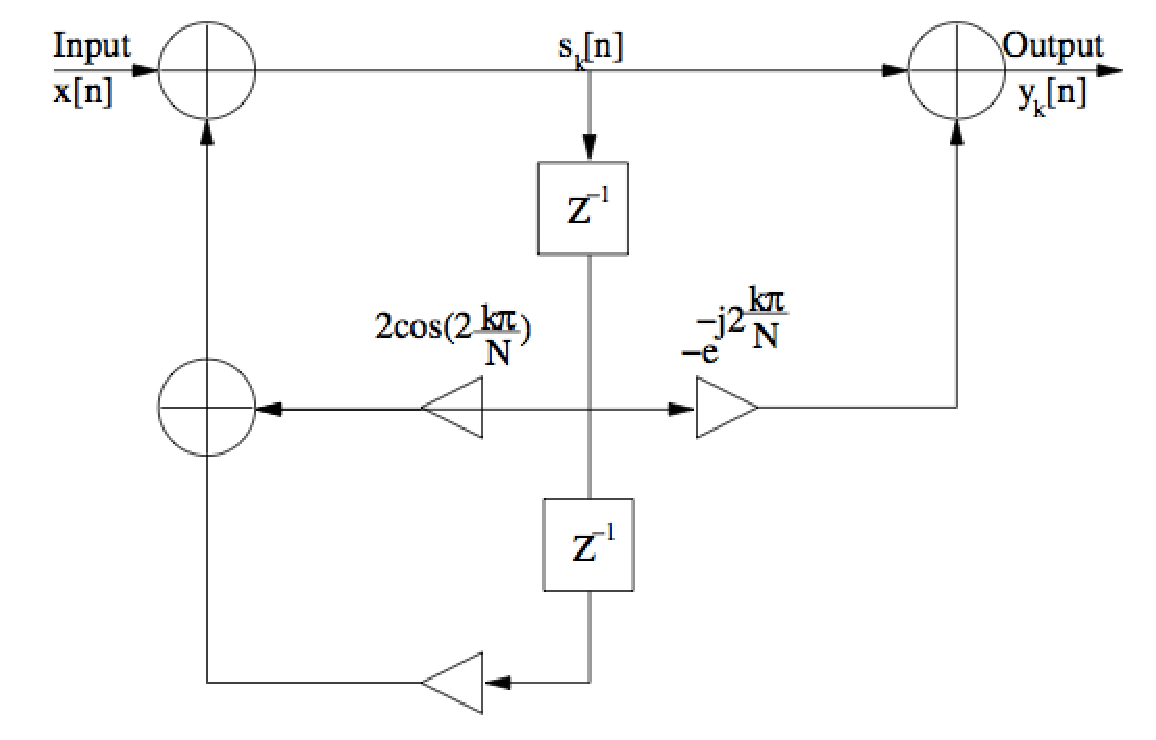
\includegraphics[width=0.5\textwidth]{IIR.pdf}
    \caption[Direct-form realisation of the Goertzel algorithm]{Direct-form realisation of the Goertzel algorithm \protect\cite{HaykinBook}.}
    \label{fig:IIR}
\end{figure}


The algorithm computes the k-th DFT coefficient $X(k)=y(N)$ of the input signal $x(n)$ using the 2nd order filter:
\begin{equation}
\begin{array}{lll}
{y_k}(n) & = & {s_k}(n) - W_N^k{s_k}(n - 1),\\
\text{with } & &{s_k}(n) = x(n) + 2\cos (\frac{{2k\pi }}{N}){s_k}(n - 1) - {s_k}(n - 2),\\
\text{and } & & {s_k}( - 1) = {s_k}( - 2) = 0

\end{array}
\label{fig:IIRtime}
\end{equation}

The discrete frequencies for which the algorithm is able to compute the DFT are ${f_k} = \frac{k}{N}{f_s}$, for $f \leq \frac{f_s}{2}$.
%%The computation for $s_k(n)$ takes one add ($x(n)-s_k(n-1)$) and one %%multiply-accumulate per received sample.

\subsubsection{Computational and Memory Complexities}

The FFT algorithm, used to compute the DFT with $N$ being a power of two, has computational demands proportional to $\mathcal{O}(N\log_2 N)$. The absolute number depends on the particular implementation. Usually the number of real-number arithmetic operations found in the literature is approximately $6N \log_2 N$. If we analyse the number of operations of the Goertzel algorithm, we realize that for a real input signal requires $N$ real multiplications and $2N$ real additions. Thus, the total number of $3N$ operations for a single frequency are required. Ignoring the computations of the cosine and the exponential constants in equation \ref{fig:IIRtime}, and for $N$ frequencies, we have that the Goertzel algorithm has quadratic complexity like the DFT. To determine for how many frequencies ($K$) it is more advantageous to exploit the Goertzel algorithm than the FFT, we compare the complexity of both and conclude that \cite{GoertzelPaper}:

\begin{equation}
3NK < 6N{\log _2}N \Leftrightarrow K < 2{\log _2}N
\label{eq:ineffgor}\ .
\end{equation}

This result holds only for $N$ being a power of two; otherwise the inequality \ref{eq:ineffgor} can even be more favourable for the Goertzel algorithm.

When only considering real inputs, the FFT algorithm requires a memory space of at least $2N$ samples. Also, the $n$ values of the transformation kernel, $\sin$ and $\cos$, are often precomputed and stored. The FFT calculation itself can be performed without moving values in the memory. However, as the computation cannot be done until the last sample of a block of data is received, a buffer size of at least $N$ samples must be used. Therefore, the overall FFT memory demand is $4N$ for real signals.
For each considered frequency, the Goertzel algorithm requires: location for saving one real and one complex state variable; the complex final output, and the last 2 real outputs $s_k(n)$ and $s_k(n-1)$. There is no need to implement input buffering because the computation can be run as the new signal samples arrive. Thereby, the total memory complexity of the Goertzel algorithm is $7K$ positions. Combining all the above together, the Goertzel algorithm will be less memory-demanding than the FFT if \cite{GoertzelPaper}.

\begin{equation}
7K < 4N \Leftrightarrow K < \frac{4}{7}N\ 
\end{equation}


As long as $N\geq 13$, equation \ref{eq:ineffgor} is decisive for choosing the best algorithm, since for these $N$ samples it holds that $\frac{4}{7} N \leq 2 \log_2 N$.


\subsubsection{Pseudo-code for Decoding Algorithm}
The pseudo-code of the implemented algorithm for the index $k$ of the DFT spectral component shown in algorithm \ref{goeralg}:  \\

\begin{algorithm}[H]
\SetKwData{Left}{left}\SetKwData{This}{this}\SetKwData{Up}{up}
\SetKwFunction{Union}{Union}\SetKwFunction{FindCompress}{FindCompress}
\SetKwInOut{Input}{input}\SetKwInOut{Output}{output}
\Input{\texttt{k; \%index of the DFT spectral component}\\
\texttt{x; \% received signal of length $\mathtt{n_{sym}}$}}
\Output{\texttt {y; \% representing $\mathtt{X[k]}$}}
\BlankLine
\texttt{\% Precalculation of constants}\;
$\mathtt{ A= 2\pi \frac{k}{N}}$\;
$\mathtt{B = 2\cos{A}}$\;
$\mathtt{C = \exp{(-j \cdot A)}}$\;
\texttt{\% State variables}\;
$\mathtt{s_0=0}$\;
$\mathtt{s_1=0}$\;
$\mathtt{s_2=0}$\;

\texttt{\% Main loop}\;
\For{{$\mathtt{i=0}$ : $\mathtt{N-1}$}}{  \texttt{\% N multiplications, 2N additions}\;
$\mathtt{s_0 = x[i] + B\times s_1 - s_2}$\;
$\mathtt{s_2 = s_1}$\;
$\mathtt{s_1 = s_0}$\;
}

\texttt{\% Finalizing calculations}\;
$\mathtt{s_0 = B\times s_1 - s_2; }$ \texttt{\% 1 multiplication and 1 addition}\;
$\mathtt{y = s_0 -s_1 \times C; }$  \texttt{\% 4 multiplications and 3 additions}\;
\BlankLine
\BlankLine
\caption{Detection algorithm for FSK: Goertzel algorithm to estimate the $k$-th spectral component of signal $x$ of length $N$.}
\label{goeralg}
\end{algorithm}


After demodulation, the decisions are sent to the decoder and the BER is computed. Denoting $n_{sym}$ as the number of samples per period, the overall rate for a 4-FSK system is given by:

\begin{equation}
R = \frac{\log_2(4)}{n_{sym}}\times f_s = \frac{2}{n_{sym}}\times f_s\ 
\end{equation}


\section{M-QAM System}
In order to meet the data throughput requirement, we considered to use a configurable M-QAM scheme to achieve the highest possible rate without compromising the performance (for instance, zero or a negligible amount of errors). In the real-time implementation, a checksum algorithm  is used to confirm the data integrity instead of FEC. However, for off-line testing different coding schemes were tested. The description of those tests and the results will be described in sections \ref{sec:ChanCodMethod} and \ref{sec:chancodresults}.
%Work on this

\subsection{M-QAM Transmitter}
\label{sub:MQAMtx}
	There are a considerable set of parameters in the transmitter that determine the performance of the system. We list the most important next:



\begin{description}{\bfseries}
  \item[\bf{$N_b$}]; number of bits to be transmitted.
  \item[\bf{$f_s$}];  sampling rate. The maximum value accepted by the phones is 44.1 kHz.
  \item[\bf{Window}]; discrete window coefficients. Each window has different parameters which will influence the impulse and frequency responses (such as the roll-off factor in the RRC or the $\alpha$ in Gaussian window).
\item[\bf{$n_{sym}$}]; number of samples per symbol. 
  \item[\bf{$levels$}]; order of the constellation. 
\item[\bf{$f_c$}]; carrier frequency. 
\end{description}


The sampling frequency, the number of samples per period and the order of the constellation will determine the rate of the system according to:
\begin{equation}
R = \frac{{2 \times levels}}{{n_{sym}}} \times f_s\ 
\end{equation}


After these parameters are set the algorithm comes into action. The first step is to merge the bits in the following order:
\[
\textbf{\texttt{bitstream = }} [\textbf{\texttt{guard band  }$\mid$\texttt{ training seq  }$ \mid $\texttt{ file headers   }$ \mid $\texttt{  data  }$ \mid $\texttt{  guard band}}]
\]

Subsequently, the bits are mapped into the constellation (MQAM) according to the pseudo-code in algorithm \ref{mod}. 


\begin{algorithm}[H]
\SetKwData{Left}{left}\SetKwData{This}{this}\SetKwData{Up}{up}
\SetKwFunction{Union}{Union}\SetKwFunction{FindCompress}{FindCompress}
\SetKwInOut{Input}{input}\SetKwInOut{Output}{output}
\Input{\texttt{bitstream; \%data to be transmitted}}
\Output{\texttt{z; \%Complex modulated symbols }$\mathtt{z = x + j \cdot y}$}
\BlankLine
\texttt{\%Initialization of vectors}\;
\texttt{mx=[]}\;
\texttt{my=[]}\;

\For{{$\mathtt{n=firstSymbol}$ \KwTo $\mathtt{lastSymbol}$}}{
\texttt{\%Initialize values of $\mathtt x_i$ and $\mathtt y_i$}\;
$\mathtt{x_i=0}$\;
$\mathtt{y_i=0}$\;
\texttt{\%Pick 2 bits of the symbol at each time}\;
\For{{$\mathtt{m=firstBit:2:lastBit}$}}{
\eIf{$\mathtt{bitstream(n+m) == 0}$}
{$\mathtt{xi = xi + 2 ^\frac{{m-1}}{2}}$\;
}{$\mathtt{xi = xi - 2 ^\frac{{m-1}}{2}}$}

\eIf{$\mathtt{bitstream(n+m+1)==0}$}
{$\mathtt{yi = yi + 2 ^\frac{{m-1}}{2}}$\;
}{$\mathtt{yi = yi - 2 ^\frac{{m-1}}{2}}$}
}
\texttt{mx=[mx xi]}\;
\texttt{my=[my yi]}\;
}
$\mathtt{z = mx + j \cdot my}$
\caption{Pseudo-code for modulation of MQAM symbols.}
\label{mod}
\end{algorithm}

 The discrete carriers to modulate the signal are generated with $n_{sym}$ samples:
\begin{equation}
\left\{ \begin{array}{l}
\cos (2\pi f_ck)\\
 - sin(2\pi f_ck)
\end{array} \right.\text{, with }  k = 0,\frac{1}{{f_s}},\cdots,\frac{{n_{sym}}}{{f_s}} - \frac{1}{{f_s}}
\label{eq:MQAMdiscCarriers}
\end{equation}

The window is also generated in the initialization of the program:
\begin{equation}\label{eq:window}
W_{n_{sym}}(i) = w_i\text{ , with }i = 1,2,\dots,n_{sym}
\end{equation}

 The coefficients $w_i$ in equation \ref{eq:window} are computed according to the previously chosen window. Then, the complex symbols, the window and the carriers are mixed together to generate the discrete transmission waveform. The generated samples for the $\emph{n-th}$ symbol have the following expression:

\begin{equation}\begin{array}{l}
s(k) = \Re (z) \cdot {W_{{n_{sym}}}}(k\% {n_{sym}}) \cdot \cos (2\pi \frac{{{f_c}}}{{{f_s}}}k) - \Im (z) \cdot {W_{{n_{sym}}}}(k\% {n_{sym}}) \cdot \sin (2\pi \frac{{{f_c}}}{{{f_s}}}k)\\
\text{with $k = n \cdot n_{sym} + 1,\cdots,n \dot n_{sym}+ n_{sym}$ ; and with \% as the modulo operator.} 
\end{array}\end{equation}

The signal $s(k)$ is then normalized to be in the range of $[-1,1]$ and converted to  \emph{short} format. In the case of the real-time implementation, the signal is sent to a buffer to be played. In the off-line mode, the signal is stored in an audio file that is saved in the phone.

\subsection{M-QAM Receiver}
\label{sub:MQAMrx}
On the receiver side, the sound samples are extracted and processed to recover the sent data. A general schematic of the receiver is illustrated in figure \ref{fig:SchemMQAMrecvr}.

\begin{figure}[h]
  \centering
    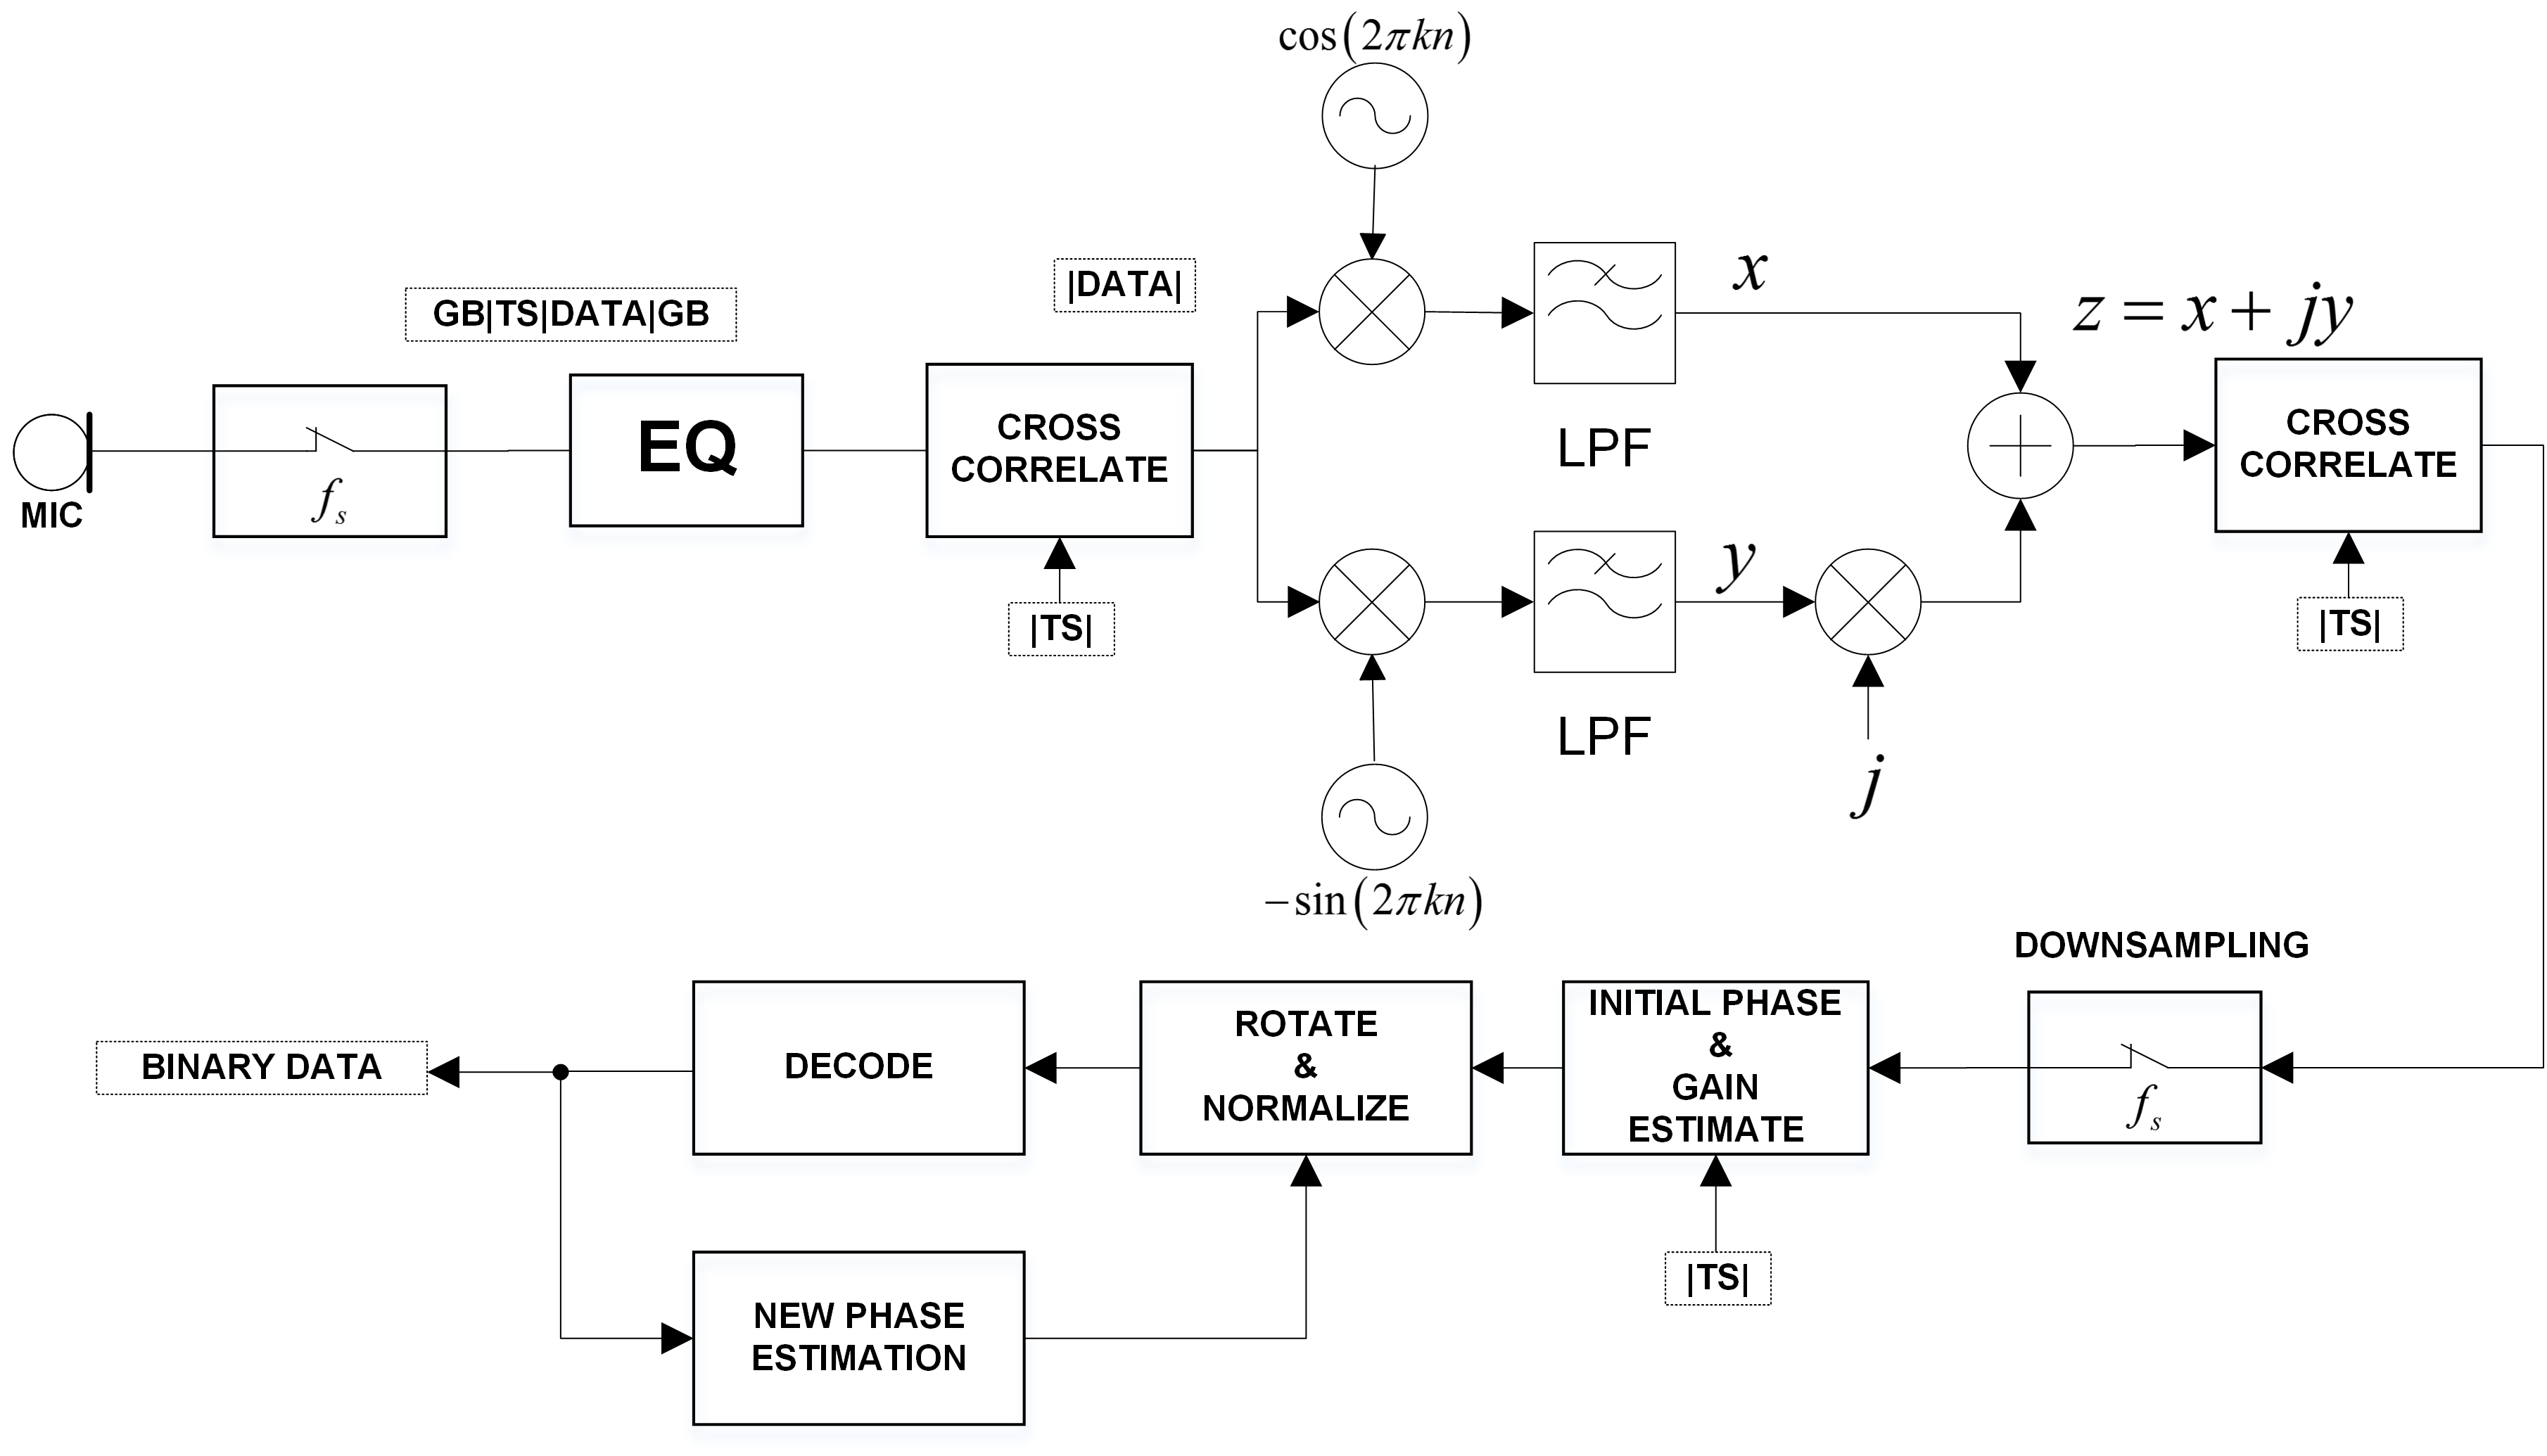
\includegraphics[width=1\textwidth]{rcvrSchem.png}
    \caption[Schematic of M-QAM receiver main processes]{Schematic of M-QAM receiver main processes.}
    \label{fig:SchemMQAMrecvr}
\end{figure}


We now describe the demodulation process. The received signal is filtered with the equaliser (EQ). The chosen equaliser is a parametric IIR filter with coefficients computed according to the process that will be described in section \ref{sec:EQdesign}. The received constellations before and after applying the equaliser are depicted in figure \ref{fig:RcvdQAMsignal}.
 

 \begin{figure}[H]
 \centering
 \begin{subfigure}{.45\textwidth}
   \centering
   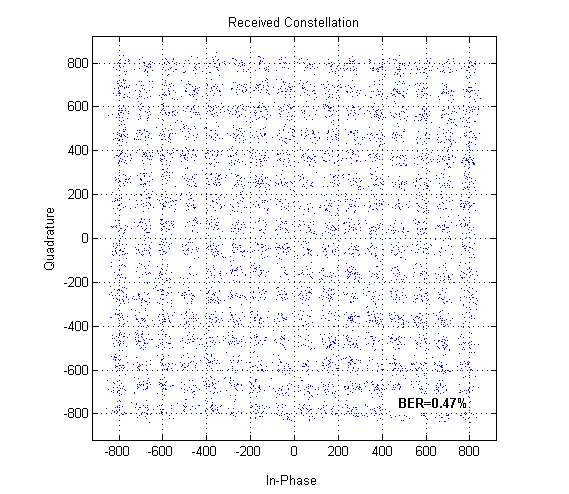
\includegraphics[width=0.9\textwidth]{rcvdNOEQ.png}
   \subcaption{Without equaliser.}
   \label{fig:ConstBeforeFilt}
    \end{subfigure}%
 \begin{subfigure}{.45\textwidth}
   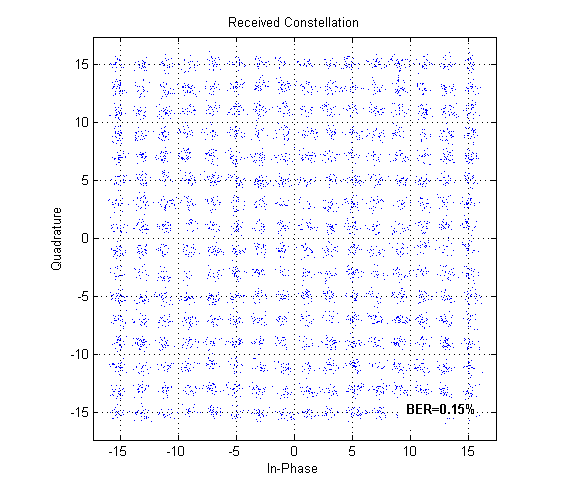
\includegraphics[width=0.9\textwidth]{rcvdEQ.png}
       \subcaption{With equaliser.}
     \label{fig:ConstAfterFilt}
    \end{subfigure}
 \caption[Received 256-QAM constellation and the effect of the equaliser]{Received 256-QAM constellation and the effect of the equaliser after phase estimation. There is a clear improvement in the BER when using the equalisation filter.}
    \label{fig:RcvdQAMsignal}
 \end{figure} 

 
 After the equalisation process, the beginning of the transmission is found by computing a sample-level cross-correlation between the modulated training sequence and the received sequence. Then, the lag $k$, which leads to the maximum value in the cross-correlation is computed and considered as the beginning of the training sequence. The samples are then multiplied by the carriers depicted in figure \ref{fig:SchemMQAMrecvr}. The next step is low-pass filtering the resulting samples. For this stage we use an order $N=12$ linear phase FIR filter modelled with the window method. The optimal parameters for the low-pass filter have been obtained iteratively based on the resulting performance and its frequency response is depicted in figure \ref{fig:LPFIR}. 
 
 \begin{figure}[h]
   \centering
     \includegraphics[width=0.8\textwidth]{LPFIR.png}
     \caption[Frequency response for LPF used in M-QAM receiver.]{Frequency response for LPF used in M-QAM receiver.}
     \label{fig:LPFIR}
 \end{figure}
 
 
At this point, the up sampled received symbols must be down sampled. The optimal choice for the sampling instants is estimated using a symbol-level cross-correlation taking into account the received symbols and the training sequence symbols as referred in section \ref{subsec:MQAMsynch}. 

The consequent steps are the blocks of phase, and channel gain estimation. The latter parameter depends on the volume of the transmitter and is assumed to be constant during the whole transmission (even though there are implemented algorithms to keep track of it). The initial phase rotation is estimated according to the algorithm mentioned in section \ref{subsec:MQAMsynch}.

To make the system robust to longer transmissions (larger file sizes), the method mentioned in section \ref{subsec:Phase rotation} is used to keep track of the Doppler shift. It consists of dividing the set of symbols into smaller subsets, to which the Maximum Likelihood (ML) decision is applied and the new phase rotation is estimated. This new phase estimation block is used to rotate the symbols in the following blocks. This algorithm assumes that the decoded symbols are correct and the added noise is zero-mean. It is important to choose a block with adequate length. It should not be either too large or too small\footnote{If the block is too large, there is a risk of error in the decoding due to the rotation leading to a wrong decision feedback. If the block is too small the assumption that the noise is zero-mean might not be accurate.}. Denoting $t$ as the interval of time in which the Doppler shift does not influence the decision, the size of the block in number of symbols is given by:
\begin{equation}
N_{block} = \frac{t}{T_s} = \frac{t\times f_s}{n_{sym}}
\end{equation}

After processing all the blocks, the decisions from each one of those blocks can be merged together and compared with the transmitted data to compute the BER. 

\subsubsection{Optimisation}

There is a number of parameters that can be adjusted that influence the performance of the system:
\begin{description}
\item[\bf EQ:] Equaliser. The gain, bandwidth and central frequency of the equaliser has a major impact in the decoding.
\item[\bf LPF:] Low-pass filter. The cut-off frequency, the order of the filter and the window used should be carefully chosen in order to suppress undesired spectral components. 
\item[\bf $t$:] Block length for decoding. The variable $t$ denotes the estimated interval of time in which the Doppler shift does not majorly influence on the decision. 
\end{description}


% % % % % % % % % % % % % % % % % % % % % % % % % % % % % % % %5}

\section{OFDM System}
\label{sec:OFDMmethod}
To overcome the fact that there is a gap around 6kHz in the channel frequency response that is slightly different in all the provided devices, an OFDM scheme is implemented. Furthermore, this modulation is able to mitigate the ISI, if the sub-carrier spacing is properly chosen. The implemented OFDM system and corresponding degrees of freedom in terms of parameters are described next.
 
\subsection{OFDM Transmitter}
\label{sub:OFDMTXmethod}
For the implementation of the OFDM system, the block schematic in figure \ref{fig:ofdmtransceiver} has been used as a reference. On the transmitter side that are a set of parameters that need to be defined:
\begin{itemize}
\item [\bf $N_{FFT}$:] The size of the FFT that is going to be used. This parameter should not be either too large or too small. Moreover, it should be a power of two\footnote{A smaller  $N_{FFT}$ will cause more overhead (due to P and S) and will hence reduce the rate. A larger $N_{FFT}$ will take more time to compute and the sub-carrier spacing will decrease leading to higher ICI.}.
%
\item  [\bf $f_c$:] The carrier frequency should be chosen so that the bandwidth of the signal remains inside the available bandwidth.
\item [\bf  $P, S$:] Cyclic prefix and suffix lengths are set according to the channel response.
 \item [\bf $N_c$:] The number of active sub-carriers will define the utilized bandwidth according to equation \ref{eq:OFDMbw}, and it is a very important parameter for the performance of the system. 

\end{itemize}

After these parameters are set and the size of the constellation is defined, the modulation algorithm takes place. In order to handle the problem of high PAPR denoted in section \ref{sub:OFDMimpairments}, a scrambler is required to spread the data signal energy. This is specially important for the case of correlated data (such as data files). The scrambling process is achieved applying a pseudo-random binary sequence with the binary operator XOR (modulo-two addition) to the original data signal. The pseudo-random sequence is generated by a linear-feedback shift register like the one depicted in figure \ref{fig:PNgenerator}.


\begin{figure}[h]
  \centering
    \includegraphics[width=0.4\textwidth]{pnSeqGen.png}
    \caption[Shift register implementation of a pseudo-random sequence generator.]{Shift register implementation of a pseudo-random sequence generator \cite{MATLABpngen}.}
    \label{fig:PNgenerator}
\end{figure}


 
 After the data is scrambled, it is merged along with the guard bits and training sequence to be mapped into the complex constellation. In the implementation, there is an option to insert pilots after each $N_{interval}$ transmitted bits. These pilot symbols, are used to re-estimate the channel. If the channel is time-invariant, better performance is obtained when such pilots are not used. Then, the symbols are introduced to the OFDM modulation function. There are $N_{FFT}$ sub-carriers for each OFDM symbol, but only $N_c$ are used (the number of virtual sub-carriers is $N_{FFT}-N_c$). Each of these blocks of size $N_c$ is split into two, and saved into the corners of a buffer of size $N_{FFT}$, as depicted in figure \ref{fig:OFDMdata}. Then, the FFT of each of these blocks is computed and cyclic prefix and suffix are added, according to the mentioned in section \ref{sec:OFDM}. Then, the resulting signal is up-converted using a complex exponential of frequency  $f_c$, and its real part is transmitted.   

\begin{figure}[h]
  \centering
    \includegraphics[width=1\textwidth]{OFDMcAdaptTX.png}
    \caption[Construction of an OFDM symbol.]{Construction of and OFDM symbol.}
    \label{fig:OFDMdata}
\end{figure}



\subsection{OFDM Receiver}
On the receiver side there is no need for equaliser, since OFDM is being used\footnote{This is because the sent training sequence allows the system to estimate the channel coefficients efficiently.}. A high pass filter might be used to cancel out the low frequency components of the noise. Next, the received signal is cross-correlated with the training sequence and the guard bands and silent parts are cropped. Afterwards, down conversion is performed using the carrier frequency exponential and, subsequently, the cyclic prefixes and suffixes are removed. To retrieve the complex transmitted symbols, the resulting samples are divided into blocks of size $N_{FFT}$ and the FFT is applied. The received training sequence symbols are compared with the ones transmitted. The phase and gain estimations are computed for each of the sub-carrier frequencies. An example of the outcome of these estimations is depicted in figure \ref{fig:OFDMphase-amp}. 

\begin{figure}[h]
  \centering
    \includegraphics[width=1\textwidth]{OFDMchannelestim.eps}
    \caption[Phase and amplitude estimation for each sub-carrier in an OFDM system.]{Phase and amplitude estimation for each sub-carrier in an OFDM system. For this example, the following parameters are used: 64-QAM constellation, $P=5$, $S=1$, $N_c=512$, $N_{FFT}=2048$, $f_c = 9 kHz$, $N_{block}=64$.
    }
    \label{fig:OFDMphase-amp}
\end{figure}


It is possible to verify the non-linearities of the channel in both amplitude and phase. Since it is known in which sub-carrier the symbols are transmitted, the corresponding phase and amplitude corrections are applied accordingly. The frequency offset correction algorithm is the same as the one used in the complex baseband implementation, and is explained in section \ref{subsec:Phase rotation}. An example of the received constellations in OFDM before and after correction is depicted in figure \ref{fig:OFDMconst}. Furthermore, if a scrambler was used at the transmission, a descrambler must be applied to recover the original data\footnote{One can use the same scrambler for the transmitter and the receiver, but they have to be initialised to the same state.}.

\begin{figure}[h]
  \centering
    \includegraphics[width=1\textwidth]{ofdm64const.eps}
    \caption[Received OFDM constellation in each sub-carrier.]{Received OFDM constellation in each sub-carrier before and after phase and amplitude correction. Each color represents a sub-carrier.}
    \label{fig:OFDMconst}
\end{figure}

\newpage
\section{Channel Coding}
\label{sec:ChanCodMethod}
Since our system is implemented purely in software, we have to use a coding scheme that does not introduce too much delay and heavy processing to the phone. On the other hand, our goal is to implement an application capable to transmit digital files, thereby we should guarantee a transmission with zero errors or being capable to correct all of them. This task is not completely straightforward, since the BER depends in many different factors that shall be analysed separately to measure the effect in the transmitted data. 
The chosen modulation scheme for our performance analysis test is 256-QAM. We have selected such configuration, since it is not possible to get an error free transmission at such rates in our implementation. 

From this point, we can introduce forward error correction into our simulation and measure the performance for different code rates. The suggested FEC implementation is a variable rate convolutional encoder with maximum free distance (according to \cite{Proakis}). The suggested code rates are: $1/2$, $2/3$, $3/4$, and $4/5$. The used generator polynomials are $[15,17]$, $[27,75,72]$, $[13,25,61,47]$, and $[237,274,156,255,337]$, respectively. There are many ways to implement such kind of functionality in software. In addition, convolutional codes have been studied for several years and there are many software implementations developed. The major challenges here are: being able to  handle different code rates, and manage the length of the data sequence. Furthermore, the Viterbi algorithm for decoding may add considerable time to the decoding process. We found an implementation in \cite{concodeSource} that is able to use different code rates with few modifications and uses the hard decision metric to decode the sent data. These functions were adapted to our system. The performance of the codes in a binary-symmetric channel (BSC) is depicted in figure \ref{fig:convBSC}.\\


\begin{figure}[h]
  \centering
    \includegraphics[width=0.6\textwidth]{bscconv.png}
    \caption[Performance of different convolutional codes in a BSC Channel.]{Performance of different convolutional codes in a BSC Channel.}
    \label{fig:convBSC}
\end{figure}


The M-QAM system was tested with such codes, and the results were not very promising. The details of the tests will be described in section \ref{sec:chancodresults}. Moreover, we could achieve a fast enough  rate without using error correction schemes. Therefore, in our  real-time implementation we opted for a checksum test instead (see section \ref{subsec:Checksum}). 


\section{Channel Equalisation}
\label{sec:EQdesign}
In order to characterise the channel and determine the best possible way to deal with the distortion that is present, we have estimated the channel transfer function with a non-parametric correlation method that has gotten us $k=45$ taps of a FIR model with order $N=k-1=44$. This process is done using MATLAB's function \texttt{impulseest}, which computes the coefficients based on a least-squares estimation algorithm \cite{MATLABimpulseest}. The resulting transfer function is plotted in figure \ref{fig:FIRtf}. 
 
 
\begin{figure}[h]
  \centering
    \includegraphics[width=1\textwidth]{FIRChanRespose.png}
    \caption[Estimated least-squares FIR model for the channel transfer function]{Estimated least-squares FIR model of the channel transfer function. The filter order is $N=44$.}
    \label{fig:FIRtf}
\end{figure}

An inverse optimal equaliser filter using this method is not stable. For this reason, the filter has to be constructed based on a parametric IIR model. The function \texttt{fdesign.parameq} constructs a Chebyshev Type I peak filter (figure \ref{fig:IIRpeak}) with the following transfer function \cite{MATLABparameq}:

\begin{equation}
H\left( z \right) = \frac{{{b_0} + {b_1}{z^{ - 1}} + {b_2}{z^{ - 2}}}}{{1 + {a_1}{z^{ - 1}} + {a_2}{z^{ - 2}}}}\ .
\end{equation}

The filter's main design parameters are the central frequency, passband bandwidth, reference gain, and passband gain. The reconstructed channel based on this approach is depicted in figure \ref{fig:cascadefilter}. There we can see that one can approximate a flat channel with stable phase response using the IIR filter in cascade. Once the parameters are defined, we obtain the coefficients from MATLAB and run an iterative process to optimize the filter to perform well in all the phones.

\begin{figure}[H]
\centering
\begin{subfigure}[H]{.8\textwidth}
  \centering
  \includegraphics[width=1\linewidth]{peakFilter.png}
  \caption{IIR peak filter.}
  \label{fig:IIRpeak}
  \quad
\end{subfigure}%
\quad
\begin{subfigure}[H]{.8\textwidth}
  \centering
  \includegraphics[width=1\linewidth]{reconstChan.png}
  \caption{Cascaded channel after filtering.}
  \label{fig:cascadefilter}
\end{subfigure}
\caption[Channel reconstruction using the IIR peak filter]{Channel reconstruction using the IIR peak filter.}
   \label{fig:chanReconstruction}
    \end{figure}

\section{Signal-to-Noise Ratio and Channel Capacity}
\label{sec:SNRmethods}
There is noise and imperfections in the channel that may introduce errors in the transmission. We have used two different approaches to measure the magnitude of the noise in comparison to the signal level. The first approach is to measure the variance of the received signal while nothing is transmitted. With the noisy samples \(n[k]\) for \(k=0,... ,N\), we calculate the mean \(\hat\mu_n\) and  the variance estimates as:

\begin{eqnarray}
                    \hat\mu_n\ & = & \frac{1}{N}\sum_{k=1}^N n[k]\\
\label{Eq:variance} \hat\sigma_n^2 & = & \frac{1}{N-1}\sum_{k=1}^N(n[k]-\hat\mu_n)^2 
\end{eqnarray}

Then, we find the maximum amplitude \(A_{m}\) of a sinusoid that can be received from the channel. After that,  we can compute the signal-to-noise ratio and obtain the channel capacity according to equation \ref{Eq:awgn_capacity}.

\begin{equation}\label{Eq:snr} \text{SNR} = \frac{A_{m}^2}{2 \hat\sigma_n^2} \end{equation}

Since we do not know if the noise have the same characteristics when the signal is present, we use a second approach which is measure the signal-to-noise-and-distortion ratio (SINAD). We again receive samples \(r[k]\) for \(k=0,... ,N\)  of a transmitted sinusoid with known frequency \(\nu_c\). The received signal is a sinusoid apart from some unknown error \(n[k]\). We can estimate the error with respect to the samples \(r[k]\) by least squares fitting a sinusoid \(a_c \cos(2\pi\nu_ck) - a_s \sin(2\pi\nu_ck)\), with the free parameters \((a_c,a_s)\). An example of the method is shown in figure \ref{fig:sinusoid_fit}. Therefore, we can use equation \ref{Eq:noise} as an estimation of the noise:

\begin{equation}\label{Eq:noise} \hat n[k] = r[k] - a_c \cos(2\pi\nu_ck) - a_s \sin(2\pi\nu_ck)\end{equation}

Next, we compute the variance of according to equation \eqref{Eq:variance} to obtain the SINAD:

\begin{equation}\label{Eq:sinad} \text{SINAD} = \frac{a_c^2+a_s^2}{2\hat\sigma_n^2}\end{equation}

\begin{figure}[H]
  \centering
    \includegraphics[width=0.7\textwidth]{sinusoid_fit.eps}
    \caption[Sinusoid carrier fit to estimate the SINAD.]{Sinusoid carrier fit to estimate the SINAD. In this example, the received signal is compared with the transmitted 500 Hz carrier.}
    \label{fig:sinusoid_fit}
\end{figure}

Using equation \ref{Eq:awgn_capacity} as reference, the approximate channel capacity using this method can now be computed as: 

\begin{equation}
\label{Eq:sinad_chan_cap} C \approx B\log_2(1+\text{SINAD})\text{                [bps]}
\end{equation}


% % % % % % % % % % % % % % % % % % % % % % % % % % % % % % % % % % % % % % % % % % % % % % % % % % % % % % % % %
% % % % % % % % % % % % % % % % % % % % % % % % % % % % % % % % % % % % % % % % % % % % % % % % % % % % % % % % %


\chapter{Results and Discussion} \label{chap:results}
We have tested several modulations schemes modulating and demodulating random binary sequences, first with MATLAB (off-line mode), and then with the phones with the provided Android Framework (real-time mode). 

In the off-line mode, transmitter and receiver processing is done solely in MATLAB. The transmitted samples (modulated signal) are sent to the phone in a file (\texttt{.dat}) of $shorts$, read by the application and delivered to the sound card buffer to be played. On the receiver side, there is a recording application which stores the audio samples in a \texttt{.log} file. The file is then transferred to the computer and the samples are extracted to be processed (demodulation).  

In the real-time mode, all the processing is done in the phones and the data that is sent is taken from a file that is converted to audio samples and then is transmitted/received with the application GUI. 

MATLAB is a powerful tool for simulation due to its computation power and adaptability and was, hence, chosen to find the optimal algorithms/methods/parameters for the implementation of a robust system. Once these methods are found they can translated into JAVA with little effort and run on the phones. If done correctly, this translation should not cause the final results to be much different in both real-time and off-line systems. 

One way to corroborate that the functions work properly is to use the \texttt{test\_harness()} method implemented in Framework. This method tests the implementation of math-intensive functions/algorithms in an isolated and repeatable way. We have followed a similar process to  verify the inputs and outputs for each of the implemented functions. In addition, Eclipse debugging tools have been used extensively to verify the correct application in run-time mode.
 

\textcolor{red}{Check.}%

\section{Binary FSK}
Our first and basic test has been to generate a random sequence and transmit it with binary FSK throughout the channel. As discussed in section \ref{sec:FSKdemod}, the Goertzel algorithm is used to decode the received modulated signal with generally good results. The maximum overall rate is about 1.764 kbps and the effective rate is 1.762 kbps for a 10kB file. We used this implementation as the initial step for our real-time application. After the system was implemented successfully, it was only used to modulate the training sequence in the 4-FSK scheme. More detailed results are presented in the next section. 


\section{4-FSK}
\subsection{Off-line Tests}
In the final implementation, 35 samples per symbol ($n_{sym}=35$) were used. The carrier frequencies were allocated according to:
\begin{equation}
{f_c} = \frac{{k \times {f_s}}}{{24}} \text{, with $k=1,4,7,10$ }
\end{equation} 
 This results in a data rate of 2.520 kbps with zero errors, considering all the bits that were transmitted, consists in a total of 110 bits. Hence, the effective rate is slightly lower than this value (2.494 kbps for a 10kB file), but still well above the basic requirements of 1 kbps. 

In figure \ref{fig:4FSKspectrum}, plots of the transmitted spectrum are shown comparing a rectangular and a Gaussian window. For both cases, the system performed with no errors, but the use of pulse shaping may allow to use a greater number of symbols. The scheme was not improved further because as we increased the number of carrier frequencies to achieve a higher rate, the system was more prone to errors. 

\begin{figure}[H]
  \centering
    \includegraphics[width=1.0\textwidth]{4FSKspectrum_windoweffect.eps}
    \caption[PSD of transmitted 4-FSK signals.]{PSD of transmitted 4-FSK signals with rectangular and Gaussian window, respectively.}
    \label{fig:4FSKspectrum}
\end{figure}


\subsection{Real-time Implementation}

As an intermediate step and in order to accomplish the mid-term requirements, we also implemented this scheme in real-time. One of the parameters that made the system more sensitive to errors was the synchronisation. For this reason, the training sequence was modulated with 2-FSK and then concatenated with the data samples modulated in 4-FSK. Although this method slightly increased the length of the transmitted signal, it helped to make sure that the detection process was more reliable. The real-time application performed equal to the off-line system in terms of implemented functions and outputs. Screenshots of the intermediate 4-FSK application are displayed in figure \ref{fig:fskscreeshots}.


\begin{figure}[H]
 \centering
 \begin{subfigure}{.3\textwidth}
 \centering
    \includegraphics[width=0.9\textwidth]{transmitFSKonline.png}
    \subcaption{Transmitter}
    \label{fig:appTXsideFSK}
    \end{subfigure}%
 \begin{subfigure}{.3\textwidth}
  	 \centering
      \includegraphics[width=0.9\textwidth]{receiveFSKonline.png}
      \subcaption{Receiver}
      \label{fig:appRXsideFSK}
   \end{subfigure}
     \caption[Screenshots of receiver and transmitter in 4-FSK application]{Screenshots of receiver and transmitter in 4-FSK application.}
     \label{fig:fskscreeshots}
 \end{figure} 


\section{4-FSK + FDM}

In order to improve the rate and exploit all the available bandwidth more efficiently, an alternative 4-FSK system with frequency division multiplexing (FDM) was designed and tested off-line. The idea was to put the frequencies in the 4-FSK scheme closer together and divide the spectrum into \(N_r\) parallel channels. \(N_r = 7\) was the highest number of channels that the system could correctly demodulate with a BER of zero. However, it was necessary to lower the rate by increasing \(n_{sym}\) to 88 samples per symbol. The resulting overall rate was:

$$ R = \frac{N_r\times \log_2(4)}{n_{sym}}\times f_s = 7 \times \frac{2}{88}\times f_s =7.02 \text{ kbps}$$


The effective rate was increased, but we had to introduce more overhead to ensure reliability. Thus, the effective rate for a 10 kB file was 6.54 kbps. This approach does increase the rate compared to the single 4-FSK system, but not at a great extent for smaller files.  A Gaussian pulse shape has been used to reduce the interference between frequencies close to each other. We have also tested the system to find the minimum number of samples per symbol needed for a zero BER with \(N_r=2,4,7\).
These results can be found in table \ref{table:FDM}. The transmitted PSD for the case \(N_r= 4\) is depicted in figure \ref{fig:4FSKFDM}.

\begin{table} [h]
\centering
\begin{tabular}{lcc} 
\hline
\bf Number of carriers \(\bf N_r\)	&  \bf{Samples per symbol}  & \bf{Rate} \textnormal{[kbps]} \\
\hline
\emph{2}        & 37           & 4.77    \\
\emph{4}        & 63           & 5.60     \\
\emph{7}        & 88           & 7.02     \\
\hline
\end{tabular}
\caption[4-FSK + FDM results for different number of FDM carriers]{4-FSK + FDM results for different values of \(N_r\)}
\label{table:FDM}
\end{table}


\begin{figure}[H]
  \centering
    \includegraphics[width=0.9\textwidth]{4FDMspectrum.eps}
    \caption[4-FSK spectrum]{Spectrum of the 4-FSK signal extended to 4 FDM.}
    \label{fig:4FSKFDM}
\end{figure}



\section{M-QAM}

\subsection{Off-line Tests}
In this implementation, the best performance was found with 64-QAM and 8 samples per symbol. A carrier frequency of 11025 Hz and a Gaussian pulse shape were used to modulate the data, giving an effective rate of 28.6 kbps when transmitting a file of 10 kB. As the size of the file gets larger, the effective rate asymptomatically increases to the limit of 33.08 kbps. This because the since the added overhead is less significant in length. The signal PSD in the transmitter and at different receiver stages are shown in figure \ref{fig:QAMsignal}.  

 \begin{figure}[H]
 \centering
     \includegraphics[width=1\textwidth]{64QAMspectrum.png}
     \caption[PSD of 64-QAM signal at different stages]{PSD of 64-QAM signal at different stages}
    \label{fig:QAMsignal}
 \end{figure} 

 The received constellation for the example above is depicted in figure \ref{fig:64qam_constellation}. The BER equals to zero in this case. If the  number of samples per symbol is reduced  to 7 in order to increase the data rate, the PSD of the signal will have a wider main lobe that exceeds the available system bandwidth. This, and other effects such as ISI makes it impossible to demodulate the signal without getting errors.
 
 \begin{figure}[h]
    \centering
     \includegraphics[width=0.8\textwidth]{64QAMscatter.eps}
     \caption[64-QAM received constellation with $BER=0$]{64-QAM received constellation with $BER=0$.}
     \label{fig:64qam_constellation}
    \end{figure}

We found that as the file size increases, the system becomes less reliable. This is mostly because the synchronisation. A possible solution for this is to add extra training sequences in the middle of the signal depending on the size of the file. However, this was not implemented.

 


\subsection{Real-time Implementation}

The 64-QAM implementation has been tested by sending different types of files of multiple sizes. At the receiver side, the check sum method (described in section \ref{subsec:Checksum}) is used to ensure that the received file is not corrupted.  In figure \ref{fig:appTXside}, a screenshot of the transmission client is displayed showing the processes that take place when sending a file, as well as the processing time of the two major transmission blocks: modulation and transmission. At the receiving side in figure \ref{fig:appRXside}, we observe the reverse process displaying a successful transmission that achieved an effective data rate of 30.7 kbps transmitting a 27 kB file. If the sent checksum is not equal to the one computed at the receiver side, an error occurs and the application triggers an error message (see figure \ref{fig:appRXsideError}).

\begin{figure}[H]
 \centering
 \begin{subfigure}{.3\textwidth}
 \centering
    \includegraphics[width=0.9\textwidth]{transmissioncomplete.png}
    \subcaption{Transmitter}
    \label{fig:appTXside}
    \end{subfigure}%
 \begin{subfigure}{.3\textwidth}
  	 \centering
      \includegraphics[width=0.9\textwidth]{filereceived.png}
      \subcaption{Receiver}
      \label{fig:appRXside}
   \end{subfigure}
    \begin{subfigure}{.3\textwidth}
     	 \centering
         \includegraphics[width=0.9\textwidth]{somethingwentwrong.png}
         \subcaption{Error message}
         \label{fig:appRXsideError}
      \end{subfigure}
     \caption[Screenshots of receiver and transmitter in M-QAM application]{Screenshots of receiver and transmitter in M-QAM application.}
     \label{fig:screenshots}
 \end{figure} 


The functions at the transmitter and at the receiver are timed to ensure that the data rate requirement is achieved. We recall that the receiver should finish decoding within $0.5\times F/C$ seconds after the transmitter has finished sending the data. Therefore, for the example above we have:

\[
T_{decoding}=0.5\times \frac{F}{C} = 0.5 \times \frac{{27.729 \times 8 \left[ {{\text{kb}}} \right]}}{{30.876\left[ {{\text{kb/s}}} \right]}} = 3.592 \left[ \text{s} \right] \geq 3.364 \left[ \text{s} \right]
\]

In this case, the decoding time constraint is met. Therefore, the system works according to the given specifications.




\section{OFDM}

The OFDM system is solely implemented in off-line mode and its objective is to achieve a data rate of 128 kbps. The whole bandwidth is used in order to maximise the rate. However, asymmetric OFDM symbols have to be used to avoid high frequency offsets. In this mode, the number of active sub-carriers around the carrier frequency is different. Furthermore, a number of active sub-carriers that is not a power of two is feasible with the current implementation. With an FFT of size $N_{FFT}=2048$ and with $N_c=800$ active sub-carriers, the occupied bandwidth results in:

$$W = \frac{N_c}{N_{FFT}}\times f_s = 17.22 kHz $$

The remaining bandwidth is used as guard band. The cyclic prefixes and suffixes lengths P and S have been found empirically. For a large number of sub-carriers or high PAPR transmissions, it is advisable to use high values for P and S. Since no up-sampling is used, the synchronisation with the training sequence is very sensitive. An error of one sample in the synchronisation may lead to a bad estimation of the channel and subsequently, provoke errors in the transmission. The big advantage in computational and performance terms, is the non usage of filters or equalisers in this implementation. Instead, only FFT's are used, which are optimised by the MATLAB built-in functions. Furthermore, this system is more reliable since it is adaptable to any type of channel (in opposition with the M-QAM system) and hence can be used with any device without loss of performance.

The guard bands, training sequences, as well as cyclic prefixes and suffixes add overhead in our system. If we denote the overhead length as $O_{len}$ and the guard bands and training sequence lengths as $G_{len}$ and $T_{seq,len}$\footnote{These lengths are in terms of symbols.}, the relation between these quantities is as follows:
\begin{equation}
O_{len} = G_{beg,len} + T_{seq,len} + G_{end,len}  
\end{equation}

Assuming $G_{len}$ and $T_{seq,len}$ to be multiples of the number of active sub-carriers $N_c$, the effective rate for the implemented OFDM system can be computed as:

\begin{equation}\label{eq:ofdmrate}
R=\frac{N_{bits}}{T_{tot}} = \frac{N_{bits}}{N_{samples}} \times f_s =
\frac{N_{bits}}{(O_{len} + \frac{N_{bits}}{2\times levels})\times \frac{S+P+N_{FFT}}{N_c}} \times f_s,
\end{equation}

The parameter $levels$ in equation \ref{eq:ofdmrate} is the number that defines the size of the constellation (for instance, $levels$ equal to 3 means a 64-QAM mapping).

Generating a binary random sequence with size $N_{bits} =800 \times N_{FFT} = 800 \times 2048 = 204.8$ kB, and setting $P=10$, $S=10$, $G_{beg,len}=8 \times N_c$, $G_{end,len}=6\times N_c N_c$, $T_{seq,len}=8\times N_c$ and $levels = 3$, the effective achieved rate is $R= 95.99 kbps $. The corresponding PSD and the constellations are depicted in figure \ref{ofdm80k}.

 \begin{figure}[H]
 \centering
\begin{subfigure}{1\textwidth}
 \centering
    \includegraphics[width=1\linewidth]{ofdm80kPSD.png}
    \caption{Transmitted and received PSD. }
    \label{fig:80psd}
\end{subfigure}%
%\begin{subfigure}{0.5\textwidth}
% \centering
 %   \includegraphics[width=1\linewidth]{ofdm80kchanest.png}
 %   \caption{Phase and amplitude estimation.}
 %   \label{fig:ofdmchanest}
 %   \end{subfigure}
 \quad
     \begin{subfigure}{0.9\textwidth}
 \centering
   \includegraphics[width=1\linewidth]{ofdm80kconst.png}
    \caption{Received constellation before and after phase and amplitude correction.}
    \label{fig:ofdm80const}
    \end{subfigure}
    \caption[Plots of an OFDM transmission at a rate of 95.99 kbps.]{Plots of an OFDM transmission at a rate of 95.99 kbps.}
    \label{ofdm80k}
\end{figure}
%[scale=0.45, trim=0 0 30cm 0, clip=true]

Now, regarding the transmission of files, we have realised the importance of using a scrambler when transmitting correlated data. A comparison of the PAPR with and without the use of a scrambler for a block of OFDM symbols is shown in figure \ref{fig:scramblers}. The usage of such blocks leads to a reduction of ICI and optimises the power that is consumed in the transmission, improving the performance.

\begin{figure}[H]
 \centering
 \begin{subfigure}{.4\textwidth}
  	 \centering
      \includegraphics[width=1\textwidth]{noscrambler.png}
      \subcaption{PAPR without scrambler}
      \label{fig:noscrambler}
   \end{subfigure}
    \begin{subfigure}{0.4\textwidth}
    \centering
       \includegraphics[width=1\textwidth]{scramblereffect.png}
       \subcaption{PAPR with scrambler}
       \label{fig:scrambleryes}
       \end{subfigure}%
     \caption[PAPR for OFDM symbols when using and not using data scrambling.]{PAPR for OFDM symbols when using and not using data scrambling.}
     \label{fig:scramblers}
 \end{figure} 

\subsection{Pushing to the limit}
The system mentioned in the previous section is very reliable and robust against synchronisation issues and large files. The trade-off here is the rate, which for large files is about 100 kbps \footnote{Still below the advanced requirements of 128 kbps due to the overhead.}. With the objective of pushing the system to the limits, we tried to increase the rate by using a larger constellation and file size. The outcome of the rate according to equation \ref{eq:ofdmrate} is plotted in figure \ref{fig:eqrate} for different file sizes and constellations. 
\begin{figure}[H]
	 \centering
\includegraphics[width=0.8\textwidth]{ratecurves.eps}
	    \caption[Rate plot for OFDM.]{Rate of the implemented OFDM system for 64 and 256-QAM and for different transmitted sizes.}
	    \label{fig:eqrate}	
\end{figure}
For a file size of 256 kB and a 256-QAM constellation, the effective rate is around the required 128 kbps. With these parameters, we are not able to guarantee an error free transmission. However, the amount of errors is very low (BER around $0.023\%$) and perfectly recoverable with a robust channel coding scheme. The constellation and the amount of errors in different sub-carriers are shown in figure \ref{fig:OFDMlast1}. In addition, a plot of the phase variation in time and frequency, and the amplitude and phase estimation are depicted in figure \ref{fig:OFDMlast2}.

 	 \begin{figure}[H]
	 \centering
	\begin{subfigure}{1\textwidth}
	 \centering
	    \includegraphics[width=1\textwidth]{256const.png}
	    \subcaption{256-QAM constellation.}
	    \label{fig:256const}	
	\end{subfigure}
	 \begin{subfigure}{1\textwidth}
		 \centering
		    \includegraphics[width=1\textwidth]{256errors.png}
		    \subcaption{Errors in time and for carrier.}
		    \label{fig:256errors}
		    \end{subfigure}
		  
	     \caption[Constellation and errors in transmission at 128kbps using OFDM.]{Constellation and errors in transmission at 128kbps using OFDM. A file with of 256kB is sent, using 256-QAM mapping. The BER for this transmission is around $0.02\%$. }
	     \label{fig:OFDMlast1}
	 \end{figure}
	 
	 \begin{figure}[H]
	 	 \centering
	    \begin{subfigure}{1\textwidth}
	 \centering
	    \includegraphics[width=1\textwidth]{surfplot.png}
	    \subcaption{Frequency-time phase estimation.}
	    \label{fig:surf}
	    \end{subfigure}
	    
	     \begin{subfigure}{1\textwidth}
	   	 \centering
	   	    \includegraphics[width=1\textwidth]{channel.eps}
	   	    \subcaption{Phase and amplitude estimation. The red line represents the carrier frequency.}
	   	    \label{fig:25chan}
	   	    \end{subfigure}
	    \caption[Frequency-time and amplitude estimation for transmission at 128 kbps.]{Frequency-time and amplitude estimation for transmission at 128 kbps. }
	    \label{fig:OFDMlast2}
	\end{figure}

 \newpage
\section{Pulse Shaping Importance}
Since we are limited in bandwidth by the channel, reduction of sidelobes via pulse shaping is a very important part of our implementation. In this section, a small comment about the use of pulse shaping in both off-line and real-time transmissions is presented.

\subsection{Real-time - M-QAM}
The complex baseband 64-QAM scheme that is implemented uses a single carrier. This leads to the existence of a main lobe and various side lobes in the spectrum of the transmitted signal. The up-conversion and down-conversion stages make these sidelobes interfere with the mainlobe. This interference is therefore minimised using efficient windowing techniques.  On the other hand, with the reduction of the number of samples per symbol, the main lobe
(which carries the information) increases its width. In our implementation we decided to use a  Gaussian window varying $\alpha$ to get the optimal value, which is computed to be  $\alpha = 2.5$. The carrier frequency  $ f_c = \frac{f_s}{4}=11025$Hz and the reduced number of samples per symbol $n_{sym} = 8$ forces the mainlobe to occupy the whole bandwidth, as depicted in figure \ref{fig:psd25}. If a rectangular or Gaussian window with $\alpha = 2$ are used, sidelobes appear interfering with the main lobe after the transmission (see figures \ref{fig:psd15} and \ref{fig:rect}). 

	 \begin{figure}[H]
	 \centering
	\begin{subfigure}[h]{0.32\textwidth}
	 \centering
	    \includegraphics[width=0.95\textwidth]{psdalfa25.eps}
	    \subcaption{Gaussian with $\alpha = 2.5$.}
	    \label{fig:psd25}	
	\end{subfigure}
	\begin{subfigure}[H]{0.33\textwidth}
	 \centering
	    \includegraphics[width=0.95\textwidth]{psdalfa15.eps}
	    \subcaption{Gaussian with $\alpha = 1.5$.}
	    \label{fig:psd15}
	    \end{subfigure}
	    \begin{subfigure}[H]{0.33\textwidth}
	 \centering
	    \includegraphics[width=0.95\textwidth]{psdrect.eps}
	    \subcaption{Rectangular window.}
	    \label{fig:rect}
	    \end{subfigure}
	    \caption[Complex Baseband Pulse Shaping]{PSD of the transmitted signal for different windows.}
	\end{figure}

\subsection{Off-line - OFDM}

In an OFDM signal, there must be a clear distinction between the mainlobe and the sidelobe in the frequency domain. In order to guarantee this, the energy  among the various active carriers should be evenly distributed. This is achieved with the implemented scrambler. In a real application such as a wireless network, OFDM signals most often follow an spectral mask\footnote{The transmitted power outside the allocated bandwidth should be below a certain threshold given by the mask.}. This can be achieve by applying a window to the transmitted OFDM symbols. This is not necessary in our case, however it has been tested. The resulting power spectral densities when using and not using a window are compared in figure \ref{fig:ofdmnowinT}.

	 \begin{figure}[H]
	 \centering
	\begin{subfigure}[h]{0.49\textwidth}
	 \centering
	    \includegraphics[width=0.95\textwidth]{ofdmnowindow.eps}
	    \subcaption{No window.}
	    \label{fig:ofdmnowin1}	
	\end{subfigure}
	\begin{subfigure}[H]{0.49\textwidth}
	 \centering
	    \includegraphics[width=0.95\textwidth]{ofdmwindow.eps}
	    \subcaption{Gaussian window applied to OFDM symbol.}
	    \label{fig:ofdmwin2}
	    \end{subfigure}
	    \caption[OFDM windowing]{Comparison of the OFDM spectrums when window is applied.}
	    \label{fig:ofdmnowinT}	
	    
	    \end{figure}

% % % % % % % % % % % % % % %
\section{Channel Coding}
\label{sec:chancodresults}

Introducing channel coding in implementations with rates below 32 kbps would only introduce a lower data throughput. In addition, we were able to achieve such rates without errors or FEC schemes. The only schemes that were be suitable for channel coding testing are 256-QAM and OFDM, as they are not able to achieve error free transmission. 
  
First, we decided to compare the performance of our MATLAB implementation with the theoretical performance of the uncoded 256-QAM in an AWGN channel. Using MATLAB's embedded function \texttt{berawgn}\footnote{Computed according to equation \ref{eq:mqamBER} from section \ref{sec:MQAMperf}.} and simulating an AWGN channel, we computed the performance of this system that turned out to be 2 dB worse than the theoretical model. The results are illustrated in figure \ref{fig:MQAMperf}. In addition, a performance curve for the rate $1/2$ code is shown in green.

 \begin{figure}[H]
  \centering
    \includegraphics[width=0.5\textwidth]{BERmix.png}
    \caption[Performance of 256-QAM system in AWGN channel.]{Performance of 256-QAM system in AWGN channel compared with the theoretical model for code rates 0 and $1/2$.}
    \label{fig:MQAMperf}
\end{figure}


The simulation shows that for the theoretical case, one can reduce the number of errors significantly. However, since the channel performance is affected by limitations other than noise, it is expected to have a greater BER in the real channel compared to the simulations. In fact, we could not achieve an error free transmission in the real-time system, even with the lowest code rate possible ($1/2 $). Furthermore, using 256-QAM with a coding scheme would get us practically the same throughput compared to the case of uncoded 64-QAM. For instance, an effective rate of 35.2 kbps can be achieved when using the $4/5$ code, but  the performance gets almost as unreliable as the uncoded 256-QAM. In order to  keep the rate high, better error correction schemes can be used by including other techniques (such as inner and outer codes, and interleaving) to ensure a reliable transmission. In the last performed test, a more powerful code of the LDPC family\footnote{Using MATLAB's communication toolbox and the coding functions \texttt{comm.LDPCEncoder} and \texttt{comm.LDPCDecoder}. The parity-check matrix for the rate $9/10$ is obtained using the function \texttt{dvbs2ldpc}.} is used. In table \ref{table:Rates}, the results are summarised comparing the error correction capabilities in terms of code rate and BER for different methods.

\begin{table} [h]
\centering
\begin{tabular}{lccccl} 
\hline
\bf{Scheme} 				& \bf Type       & \bf{Raw data rate}\textnormal{ [kbps]}    & \shortstack{\bf{Effective data rate}\\ \bf{@ 10kB}\textnormal{[kbps]}} &  \bf{BER} \\
\hline
\emph{256-QAM, FEC:$1/2$}   & Convolutional    & 44.10           			 & 19.97        & 2.37$\times 10^{-5}$    \\
\emph{256-QAM, FEC:$3/4$}   & Convolutional    & 44.10        		         & 28.60        & 5.52$\times 10^{-5}$    \\
\emph{256-QAM, FEC:$4/5$}   & Convolutional    & 44.10      			     & 35.21        & 2.22$\times 10^{-4}$    \\
\emph{256-QAM, NO FEC}      & N/A              & 44.10       			     & 36.49        & 2.88$\times 10^{-4}$    \\
\emph{256-QAM, FEC:$9/10$}  & LDPC             & 44.10     			         & 39.61        & 1.45$\times 10^{-5}$    \\
\hline
\emph{64-QAM, NO FEC}       & N/A              & 33.08            			 & 28.60        & $\sim 0$  			  \\
\hline
\end{tabular}
\caption[Performance of different modulation/coding schemes]{Performance of different modulation/coding schemes.}
\label{table:Rates}
\end{table}




\section{Signal-to-Noise Ratio Measurements}

Both measurement methods described in section \ref{sec:SNRmethods} are evaluated on received signals of length \(N = 441000\) samples corresponding to a signal of \(10\) seconds. For the SINAD measurement, a sinusoid with frequency \(11025\) Hz \((f_s/4)\) is used. The histogram of the residual noise in the SINAD measurement is depicted in figure \ref{fig:noise_histogram}. This figure shows that the noise can be approximated to a Gaussian distribution. The resulting values of SNR and SINAD measurements are enlisted in table \ref{table:snr}.


\begin{table} [h]
\centering
\begin{tabular}{lcc} 
\hline
\bf{Method}	& \bf{Measured value }\textnormal{[dB]}    & \bf{Channel Capacity }\textnormal{[kbps]} \\
\hline
\emph{SNR}          & 51.19            & 375.8       \\  
\emph{SINAD}        & 29.71            & 218.1       \\   
\hline
\end{tabular}
\caption[Channel Capacity with different SNR measurements]{Channel Capacity with different SNR measurements.}
\label{table:snr}
\end{table}


\begin{figure}[H]
  \centering
    \includegraphics[width=0.7\textwidth]{snr_noise_histogram.eps}
    \caption[Histogram of the channel residual noise.]{Histogram of the channel residual noise while transmitting a sinusoid in the SINAD measurement.}
    \label{fig:noise_histogram}
\end{figure}


\section{Summary of Results}

\begin{table} [h]
\centering
\begin{tabular}{lcccccccc} 
\hline
\shortstack{\bf Mod. \\ \bf scheme} &  \bf{Tested}  & \shortstack{\bf Upsample\\ \bf factor} & \shortstack{\bf File \\ \bf Size }& \bf Coding & \bf \shortstack{\bf TS\\\bf length} & \shortstack{\bf GB \\\bf length} & \bf EQ  & \shortstack{\bf{Effective}\\\bf{Rate}\textnormal{ [kbps]}}\\
\hline
\emph{4-FSK}            &  Off-line             &    35        &  10 kB  &    No   &  300 bits   &  100 bits     &  No  & 2.49  \\  
\emph{4-FSK}            &  Real-time            &    35        &  10 kB &    No   &  100 bits   &  40 bits      &  No  & 2.51  \\  
\emph{4-FSK/FDM}      &  Off-line             &    88        &  10 kB &    No   &  200 bits   &  200 bits     &  No  & 2.51  \\  
\hline
\emph{64-QAM}            &  Off-line             &    8         &  10 kB  &    No   &  500 sym &  540 sym &  No  & 29.57   \\  
\bf\emph{64-QAM}            &  Real-time            &    8         &  27 kB &    No   &  200 sym &  520 sym &  No  & 30.88   \\
\hline
\bf\emph{OFDM}             &  Off-line             &  \shortstack{1, $P=10,$ \\ $S=10$}&  205 &    No   &  8 sym &  8 sym &  No  & 95.99 \\
\hline
\end{tabular}
\caption[Summary of results with $BER=0$.]{Summary of results with $BER=0$.}
\label{table:results}
\end{table}


% % % % % % % % % % % % % % % % % % % % % % % % % % % % % % % % % % % 
% % % % % % % % % % % % % % % % % % % % % % % % % % % % % % % % % % %
\chapter{Conclusions}
\label{chap:conclusions}

\section{Transceiver Overview}

The task that was given was to implement a file transfer system using an audio channel. From the transceiver implementation point of view, we have started from the initial design steps to the system deployment. We began by studying possible modulation/demodulation techniques and inferred that FSK, complex baseband M-QAM and OFDM were the best candidates.  The implementation of those systems was successfully done and the performance results of both, the off-line and real-time system were equal. An overview of the results will be described below as well as further possible improvements. 

There is always a trade-off between reliability and data rate in a communications system. In our implementation, we tried to balance this trade-off always aiming to the parameters that maximised the throughput but led us to the lowest amount of errors (zero). The chosen system guaranteed us a reliable and fast transmission scheme that exploited the available resources efficiently. We were able to achieve a rate of 33kbps in the real-time system with a reliable implementation of a 64-QAM system. On the other hand, an OFDM scheme with 64-QAM mapping was tested off-line, allowing us to almost triplicate the rate (96 kbps) that was achieved previously. 
\textcolor{red}{We have learned a lot blah blah.} Finally, this project along with 

\section{Channel Properties}
The audio channel that we worked is non-linear with presence of amplitude and phase distortion (there is an amplitude gap around 6kHz). Moreover, it has frequency offsets as the local oscillators in both phones are not aligned. Furthermore, the effective available bandwidth is small (around 21 kHz). On the other hand, the noise is well modelled by a low variance, zero-mean AWGN and the phase varies slowly in time. To estimate the initial phase rotation, a medium-sized training sequence is used. To keep track of the frequency offset, the fact that the SNR is high is exploited, and a decision feedback algorithm has been implemented.

The amplitude distortion was corrected with an IIR peak filter that equalised the gap and performed well with different phones. In addition, it did not introduce larger complexity or additional distinguishable distortion to the transmitted signal.

\section{Further Improvements}
In the implementation of the various systems, we looked forward to improve them and optimise the corresponding parameters. However, due to time and other constraints, there are few things that were not fully implemented. 
First constraint was imposed by the provided cable and the phones' sound card architecture, which allow only half-duplex transmissions. If a full-duplex system was given, a transmission control protocol could have been executed. Another physical limitation was the mono playback of the audio. If the left and right channels were available, the rate could have been doubled, given there is no cross-interference. 

Secondly, more efficient channel and source coding schemes could have been implemented to improve the system performance. In this way, the limit of 128 kbps could have been achieved using larger file sizes and efficient channel coding. The simulations that we have run with the real-time system show that its performance was around 2dB worse than the theoretical system.  Even though the designed frequency offset tracker performed well, other solutions are available such as the use of adaptive equalisers and filtering. In addition, the tests using error correction codes indicate that in order to achieve a good performance other techniques shall be used jointly to recover the sent data.  

Finally, there were other design and hardware limitations that hindered our progress. The real-time system was designed in such a way that it was not possible to send files larger than \textcolor{red}{36kB}. This constraint was imposed mainly by the phone memory management and the usage of large audio buffers to send and receive the processed data. Therefore, a different implementation choice could have solved this issue and would had allowed us to send files of any size. Minor constraints with the allocated space for the headers also limited the length of the strings that could be used in these fields.  





\begin{thebibliography}{1}
\bibitem{report2012}
EQ2430 Project Course in Signal Processing and Digital Communications, Green Group, \emph{EQ2430: In-Flight File Transfer  [Final Report]}, KTH, 2012.


\bibitem{Madhow}
Madhow U., \emph{Fundamentals of Digital Communication}, Cambridge , 2008.

\bibitem{Proakis}
Proakis J. ,Salehi Masoud, \emph{Digital Communications}, McGraw-Hill , 2008.

\bibitem{ASKDemGaza}
Abu M., \href{http://site.iugaza.edu.ps/mabufoul/files/2010/09/Experiment-5.pdf}
{\emph{ASK demodulator [Lab Experiment]}},
Islamic University of Gaza, retrieved in April 2014.


\bibitem{DigModTech}
Sa-nguankotchakorn T. , \href{http://www.tc.ait.ac.th/faculty/teerapat/AT77.11_Digital\%20Modulation\%20Techniques/III.Frequency_Shift_Keying.pdf}{\emph{Frequency Shift Keying [Lecture Slides]}}, Asian Institute of Technology, retrieved in April 2014.


\bibitem{DigCommLec}
Okechukwu C. Ugweje, \href{ugweje/web/Courses/Ee549/Handout/EE549F01Lecture37.pdf}{\emph{Frequency Shift Keying [Lecture Slides]}},  University of Akron, retrieved in April 2014.


\bibitem{XiongDigModTech}
Xiong F., \emph{Digital Modulation Techniques}, Artech House, 2006.

\bibitem{gold}
Shembil S., \emph{M-Ary FSK with Orthogonal Pulse Envelopes and its Noncoherent Detection}, IJECS-IJENS, Vol. 10, No.06, Issued December 2010, pp. 103-106.

\bibitem{GoertzelPaper}
Sysel and Rajmic, \emph{Goertzel algorithm generalized to non-integer multiples of fundamental frequency}, EURASIP Journal on Advances in Signal Processing, 2012, 2012:56.

\bibitem{ProjectEQ2310}
EQ2310 Digital Communications, \emph{Analysis and Simulation of a QPSK System [Project Assignment ]}, KTH, 2013.

\bibitem{EQ2440ProjectDescription}
EQ2320 Project in Wireless Communication, \emph{Project \#1: In-flight file-transfer using 3-mm cable [Project Description]}, KTH, 2014.

\bibitem{HaykinBook}
Haykin S., \emph{Digital Communication Systems}, John Wiley \& Sons, Inc., 2014.

\bibitem{CarrierSynchPaper}
Dick D., Harris F., and Rice M., \emph{FPGA Implementation of Carrier Synchronization for QAM Receivers}, Journal of VLSI Signal Processing 36, 57-71, 2004.

\bibitem{NI QAM white-paper}
National Instruments, (2012), \href{http://www.ni.com/white-paper/3896/en/}{\emph{Quadrature Amplitude Modulation (QAM)[White paper]}}, retrieved in May 2014.

\bibitem{Agilent IQ paper}
Agilent Technologies, (2013) \href{http://wireless.agilent.com/wireless/helpfiles/89600B/WebHelp/subsystems/digdemod/content/digdemod_para_interact_iqgainimb_quadskewerr.htm}{\emph{IQ Gain Imbalance and Quadrature Skew Error Data Interaction (Digital Demod)[9600 VSA Software - Product Documentation]}}, retrieved in May 2014.

\bibitem{BER-QAM paper}
Yoon D., Cho K., and Lee J., \emph{Bit Error Probability of M-ary Quadrature Amplitude Modulation}, Vehicular Technology Conference, 2000. IEEE-VTS Fall VTC 2000. 52nd , vol.5, no., pp.2422,2427 vol.5, 2000.
\bibitem{DSPDiniz}
Diniz P., Da Silva E., Netto S., \emph{Digital Signal Processing: System Analysis and Design}, Cambridge University Press, 2010.

\bibitem{SklarBook}
Sklar B., \emph{Digital Communications Fundamentals and Applications}, Prentice Hall, 2001.

\bibitem{ConvCodesTut}
Langton C., \href{http://complextoreal.com/wp-content/uploads/2013/01/convo.pdf}{\emph{Coding and decoding with Convolutional Codes [Tutorial] }}, Complex To Real Website, retrieved in April 2014. 

\bibitem{concodeSource}
Rong Su, R., \href{http://mis.knjc.edu.tw/~ronald/course/matlab/Matlab-source/communication/71ca84878640/all_chapters/Chapter8/}{\emph{Matlab Source Code repository}}, Department of Information Management, Kang-Ning Junior College of Medical Care and Management, Taiwan, retrieved in April 2014.

\bibitem{UMLref}
Booch G., Rumbaugh J., Jacobson I., \emph{The Unified Modeling Language User Guide}, Addison-Wesley, 2005.

\bibitem{MATLABpngen}
The MathWorks Inc. , \href{http://www.mathworks.se/help/comm/ref/pnsequencegenerator.html}{\emph{PN Sequence Generator [Documentation]}},  2014.


\bibitem{MATLABimpulseest}
The MathWorks Inc. , \href{http://www.mathworks.se/help/ident/ref/impulseest.html}{\emph{\texttt{impulseest}: Nonparametric impulse response estimation [Documentation]}}, 2014.

\bibitem{MATLABparameq}
The MathWorks Inc. , \href{http://www.mathworks.se/help/dsp/ref/fdesign.parameq.html?searchHighlight=fdesign.parameq}{\emph{\texttt{fdesign.parameq}: Parametric equalizer filter specification [Documentation]}},  2014.


\bibitem{FFTJavaRef} 
Robert Sedgewick and Kevin Wayne,
\href{http://introcs.cs.princeton.edu/java/97data/FFT.java.html}{\emph{\texttt{FFT.java} [Documentation]}},  Princeton, 2011, retrieved in April 2014.

\bibitem{ComplexJavaRef} 
Robert Sedgewick and Kevin Wayne,
\href{http://introcs.cs.princeton.edu/java/97data/Complex.java.html}{\emph{\texttt{Complex.java}[Documentation]}},  Princeton, 2011, retrieved in April 2014.


\bibitem{Checksumref1} 
Braden R.,
Borman D., 
Partridge C., 
\href{http://tools.ietf.org/html/rfc1071}{\emph{Computing the Internet checksum [Memo]}}, Networking Working Group IETF,
September 1988, retrieved in May 2014.


\bibitem{Checksumref2}
Plummer W., \emph{TCP Checksum Function Design}, SIGCOMM Comput. Commun. Rev., 57-71, 1989.

%% Slides & handouts



\end{thebibliography}


\end{document}